\documentclass[12pt,oneside,letterpaper,spanish]{report}
\usepackage[utf8]{inputenc}
\usepackage[T1]{fontenc}
\usepackage{csquotes}
\usepackage[margin=2.25cm,headheight=26pt,includeheadfoot]{geometry}
\usepackage[spanish]{babel}
\usepackage{listings}
\usepackage{color}
\usepackage[pagestyles]{titlesec}
\usepackage{titling}
\usepackage[framed, numbered]{matlab-prettifier}
\usepackage{changepage}
\usepackage{amsmath}
\usepackage{enumitem}
\usepackage{graphicx}
\usepackage{fancyhdr}
\usepackage{lastpage}
\usepackage{caption}
\usepackage{tocloft}
\usepackage{setspace}
\usepackage{multirow}
\usepackage{float}
\usepackage{comment}
\usepackage{booktabs}
\usepackage{indentfirst}
\usepackage{lscape}
\usepackage{booktabs,caption}
\usepackage[flushleft]{threeparttable}
\usepackage[english]{nomencl}
\usepackage{xcolor}
\usepackage{lipsum}
\usepackage{array}
\usepackage{natbib}
\usepackage{tikz}
\usepackage[hidelinks]{hyperref}
\usepackage{amsthm}
\usepackage{amssymb}
\usepackage{tcolorbox}
\usepackage{listings}
\usepackage{multicol}
\usepackage{footnote}
\usepackage{array}

% Habilita 3 niveles de profundidad
\setcounter{tocdepth}{3}
\setcounter{secnumdepth}{3}

% Comando para eliminar 'Capítulo N' de \chapter{}
\titleformat{\chapter}[display]{\normalfont\bfseries}{}{0pt}{\Huge}
\newpagestyle{mystyle}
{\sethead[\thepage][][\chaptertitle]{}{}{\thepage}}
\pagestyle{mystyle}

% Comando para agregar ambientes de teorema
\newtheorem*{theorem}{Teorema}

% Definir el color azul
\definecolor{myblue}{RGB}{54, 95, 145}

\newtcolorbox{mybox}[1]{colback=white, colframe=myblue, fonttitle=\bfseries, title=#1}

% --- set footer and header ---
\pagestyle{fancy}
\fancyhf{}

\setlength{\parindent}{2em}
\title{Proyecto Estadística I} % to reference as \title, dont use \maketitle
\makeatletter\let\Title\@title\makeatother

\lstset{language=Matlab,
style=Matlab-editor,
basicstyle=\normalsize\mlttfamily,
numbers=left,
numberstyle={\scriptsize\color{black}},	% size of the numbers
numbersep=0.5cm											
}

\newlist{steps}{enumerate}{1}
\setlist[steps, 1]{leftmargin=1.5cm,label = Step \arabic*:}

\renewcommand{\rmdefault}{ptm}
\renewcommand{\headrulewidth}{1pt}
\renewcommand{\footrulewidth}{1pt}
\lhead{\Title}
\rhead{\nouppercase{\rightmark}}
\lhead{\Title}
\setlength\headheight{16pt}
\setlength{\footskip}{50pt}
\lhead{\Title} %rightH title
\cfoot{\thepage}

% --- End of page settings ---

% -------------------------------
% --- Acá inicia el documento ---
% -------------------------------

\begin{document}
\pagenumbering{roman} 
\begin{titlepage}
\begin{center}
\vspace{2cm}

\includegraphics[width=0.2\textwidth]{root/Logo_ucr.png}~\\[1cm]

{\huge Universidad de Costa Rica} \\
{\large 
Escuela de Matemáticas \\
Estadística Actuarial I \\
CA-0303\\
}

\vspace{.5cm}


\hrule
\vspace{.5cm}
{ \Huge \bfseries Proyecto - Bitácora II} 
\vspace{.5cm}
\hrule
\vspace{1cm}

{\Large \textbf{Relación entre los indicadores de progreso socioeconómico y el índice de felicidad de los países}}
\vspace{1cm}

\textsc{\textbf{Profesor}}\\
\vspace{2px}

Maikol Solís Chacón PhD \\

\vspace{.5cm}
\textsc{\textbf{Estudiantes}}\\
\vspace{2px}


Luis Fernando Amey Apuy - C20470\\
\vspace{5px}
Anthony Jiménez Navarro - C24067\\
\vspace{5px}
Javier Hernández Navarro - C13674\\
\vspace{5px}
Erick Venegas Espinoza - C09319\\

\vspace{1cm}

I - 2024 \\


\end{center}
\end{titlepage}

\newpage
\doublespacing
\renewcommand{\baselinestretch}{1}\normalsize
\tableofcontents
\renewcommand{\baselinestretch}{1}\normalsize
\singlespacing
\thispagestyle{fancy} % force page style

\newpage
\pagenumbering{arabic} 
\fancyfoot[C]{Página \thepage\ de \pageref{EndOfText}}

% --- Bitácora 1 ---
\chapter{Bitácora 1} \label{bitacora1}

\section{Parte de planificación} 
\subsection{Pregunta de investigación}

\subsubsection{Definición de la idea} 

La idea central es examinar la relación entre el progreso socioeconómico de un país (representado por variables como acceso a la electricidad y al agua, PIB per cápita, entre otros) y el Índice de Felicidad de sus habitantes. Para llevar a cabo lo anterior se utilizará el método delta, con el que se buscará aproximar la distribución de la variable aleatoria del Índice de Felicidad, para así comprender mejor su comportamiento y potencialmente obtener información sobre factores predictivos o determinantes de la misma en contextos socioeconómicos. 

\begin{itemize}
    \item \textbf{Están interesados en el tema:} El interés en este tema radica en la comprensión de cómo el progreso socioeconómico de un país se relaciona con el bienestar y la felicidad de sus ciudadanos. Al entender mejor las conexiones entre estos aspectos, podemos identificar áreas de mejora, diseñar estrategias de desarrollo más inclusivas y equitativas, y promover un crecimiento económico que beneficie verdaderamente a toda la sociedad.

    \item \textbf{Es relevante bajo el contexto del curso:} Este tema es relevante ya que proporciona una oportunidad de aplicar los conceptos y técnicas aprendido en clase en un contexto real y significativo. La exploración de la relación entre el progreso socioeconómico y la felicidad de una población implica analizar múltiples variables y entender cómo se distribuye la variable aleatoria del Índice de Felicidad.

    \item \textbf{Ya hicieron una investigación rápida del tema:} Sí, y afortunadamente es un tema que ofrece una amplia gama de resultados, desde artículos científicos, comparaciones entre países por región, estudios de gran relevancia, entre otros. Por ejemplo, en el artículo llamado \textit{Crecimiento económico, progreso social y felicidad} (Montuschi, 2017) se fundamenta la importancia de considerar índices de felicidad como indicadores de progreso de un país. Mientras que en el artículo titulado \textit{Movilidad social, preferencias redistributivas y felicidad en Colombia.} (Londoño, 2011) se observa cuál es el estrato que posee mayor felicidad con respecto a la movilidad, ingreso y justicia social, relacionando estas variables.
    
    \item \textbf{Es una idea específica, pero no demasiado en caso de querer abordar otros métodos o puntos de vista:} El tema en sí ofrece un amplio panorama para investigar, ya que a partir de los indicadores de bienestar de cada país, se pueden llevar a cabo múltiples enfoques para diversas investigaciones. En este caso, al centrarnos en buscar una relación entre el progreso económico y el Índice de Felicidad, estaríamos delimitando el tema, pero siempre dejando abierta la opción de agregar o profundizar más en todo el panorama que ofrece. 
\end{itemize}

\newpage
\subsubsection{Conceptualización de la idea}

Para llevar a cabo la conceptualización de la idea, comenzaremos por definir cada una de las palabras presentes en ella, para ello se utilizará el diccionario de la \textit{Real Academia Española} [RAE] \footnote{[RAE]: \cite{rae}}.

\begin{itemize}
    \item \textbf{Relación:} [RAE] Conexión, correspondencia de algo con otra cosa. 
    
    \item \textbf{Progreso:} [RAE] Acción de ir hacia adelante.

    \item \textbf{Socioeconómico:} [RAE] Perteneciente o relativo a los factores sociales y económicos.
    
    \item \textbf{País:} [RAE] Territorio, con características geográficas y culturales propias, que puede constituir una entidad política dentro de un Estado.

    \item \textbf{Índice:} [RAE] Expresión numérica de la relación entre dos cantidades.

    \item \textbf{Felicidad:} [RAE] Estado de grata satisfacción espiritual y física.

    \item \textbf{Habitantes:} [RAE] Cada una de las personas que constituyen la población de un barrio, ciudad, provincia o nación.

    \item \textbf{Distribución:} [RAE] Función que representa las probabilidades que definen una variable aleatoria o un fenómeno aleatorio.

    \item \textbf{Variable aleatoria:} [RAE] Variable que tiene asociada una determinada ley o distribución de probabilidad, en la que a cada uno de los valores que puede tomar le corresponde una frecuencia relativa o de probabilidad específica. 

    \item \textbf{Comportamiento:} [RAE] Manera de comportarse. 

    \item \textbf{Información:} [RAE] Comunicación o adquisición de conocimientos que permiten ampliar o precisar los que se poseen sobre una materia determinada.

    \item \textbf{Factores:} [RAE] Elemento o causa que actúan junto con otros.

    \item \textbf{Predictivos:} [RAE] Que predice o sirve para predecir.
    
\end{itemize}

\newpage
\subsubsection{Identificación de tensiones}

Un posible tensor en la investigación podría surgir de la complejidad de las variables involucradas en la relación entre el progreso socioeconómico y el Índice de Felicidad. Esto se debe a que estas variables pueden ser polifacéticas y estar influenciadas por una variedad de factores culturales, sociales y económicos. Con ello también entran problemas locales de países, donde no se puede generalizar a una base de datos para tomar en cuenta una felicidad agregada, esto por la falta de indicadores como el acceso a las necesidades básicas, la capacidad de proporcionar empleo, la alfabetización, la corrupción, el servicio de salud, entre otros, puede ser problemático para realizar una conclusión general. Tener en consideración estos datos puede ser crucial para poder comprender ciertos patrones y resultados.\\

Otra tensión que podría surgir de manera directa es el hecho de conseguir datos de calidad, los cuales serán indispensables para llevar a cabo el análisis. Obtener datos confiables y actualizados sobre el progreso socioeconómico y el nivel de felicidad de una población puede ser un desafío, especialmente con los países que disponen de sistemas de recolección de datos menos desarrollados o donde existen limitaciones como lo es la transparencia de la información.\\

También se tiene la controversia al intentar interpretar o medir la felicidad de un país, esto porque la felicidad es un concepto subjetivo y culturalmente variable, lo que dificulta su cuantificación y comparación entre diferentes contextos. Así mismo, la reciente popular idea sobre unir la felicidad y progreso económico mantienen un pensamiento arraigado en la sociedad, el cual, como se han visto en diferentes artículos, se puede llegar a dividir levemente entre un pensamiento de esfuerzo social y progreso en desarrollo.\\

Por otro lado, encontrar una distribución adecuada para la felicidad es un dilema, no sólo estadístico, si no a nivel de definición. Esto podría suceder en caso de encontrarse resultados contradictorios en las correlaciones, pero estos mismos al mismo tiempo definen mejor la distribución de la variable. A su vez, considerando que la base de datos presenta observaciones reducidas, las correlaciones pueden no aportar mucha información conforme a las conclusiones; hay que proceder con cuidado en cómo definir las variables y así lograr concluir información con coeficientes de correlación nivelados. \\  

\subsubsection{Reformulación de la idea en forma de pregunta}

\begin{itemize}
    \item ¿Existe una relación positiva entre el PIB per cápita y el Índice de Felicidad de las personas?
    \item ¿De qué manera resulta importante el progreso socioeconómico para un país?
    \item ¿Cómo se relacionan las variables socioeconómicas con el Índice de Felicidad?
    \item ¿Resulta relevante la distribución del Índice de Felicidad para conocer otros factores?
\end{itemize}

\newpage
\subsubsection{Argumentación de las preguntas}

\textbf{Pregunta 1:} ¿Existe una relación positiva entre el PIB per cápita y el Índice de Felicidad de las personas?
\begin{itemize}
    \item Contraargumentos:
    \begin{itemize}
        \item \textbf{Lógica}: La relación a determinar entre el PIB per cápita y el Índice de Felicidad de las personas puede ser un proceso más complejo. La distribución desigual que puede experimentar este podría significar que no todos los habitantes de un territorio gocen de un aumento en el Índice de Felicidad.
        \item \textbf{Ética}: El utilizar el crecimiento económico como medida del progreso de una sociedad y su relación con la felicidad de sus habitantes pueden ser contraproducente ya que el avance económico tiene relación con la explotación de recursos naturales y una falta de consideración con respecto al bienestar social a expensas de un mayor beneficio económico.
        \item \textbf{Emocional}: Un enfoque central en el desarrollo económico podría resonar de forma negativa para poblaciones de estratos sociales marginalizados, así como para los individuos que se encuentran en situaciones laborales inadecuadas o en un estado de explotación laboral.
    \end{itemize}
    \item Argumentos:
    \begin{itemize}
        \item \textbf{Lógica}: El PIB per cápita representa un componente importante para medir el desarrollo de territorios. De igual forma, países mas desarrollados tienden a presentar un PIB per cápita mayor, además de servicios médicos de calidad superior en comparación a países subdesarrollados, lo cual se relaciona de forma positiva con el Índice de Felicidad a lo largo del planeta.
        \item \textbf{Ética}: Con gobiernos transparentes, un aumento del PIB per cápita, se vería reflejado un aumento equitativo generalizado del bienestar social, lo que a su vez ha demostrado presentar una relación positiva con respecto a la felicidad reportada de los individuos.
        \item \textbf{Emocional}: Aunque la relación existente entre el aumento del bienestar económico y la felicidad se observa como un proceso complejo y polifacético, el aumento del PIB per cápita tiene un efecto directo en la seguridad económica de los habitantes así como un sentimiento de estabilidad.
    \end{itemize}
    \item Conclusión: La relación existente entre el PIB per cápita es un proceso complejo y polifacético. Aunque este puede tener cierta influencia sobre la felicidad, es necesario llevar a cabo un análisis más complejo que tome en cuenta una multiplicidad de variables distintas, tanto situaciones éticas, emocionales como sociales y económicas.
\end{itemize}

\newpage
\textbf{Pregunta 2:} ¿De qué manera resulta importante el progreso socioeconómico para un país?
\begin{itemize}
    \item Contraargumentos: 
    \begin{itemize}
        \item \textbf{Lógica}: La relevancia del progreso socioeconómico puede no resultar de gran importancia para un país, dados muchos casos y contextos. La estabilidad política de un país o ambiental son cruciales en las últimas décadas, para prevenir guerras o desastres ecológicos. En conjunto a eso, la importancia puede ser variada, dependiendo de muchos factores y no solo apuntando a uno central.  
        \item \textbf{Ética}: El progreso socioeconómico puede resultar subjetivo, inclusive entre las variables tomadas en cuenta en el estudio, por lo que se debe continuar con precaución para no presentar una conclusión específica, puesto que se puede excluir algunos grupos selectos.
        \item \textbf{Emocional}: La implementación de la metodología en cuestión puede ser inadecuada e imprecisa en general, donde el progreso socioeconómico puede no reflejar las problemáticas reales del país.
    \end{itemize}
    \item Argumentos:
    \begin{itemize}
        \item \textbf{Lógica}: Es crucial el progreso tanto social como económico en un país, puesto que al mismo tiempo que se crece en recursos económicos y hay más poder adquisitivo y por lo tanto comodidad, la sociedad crece en volumen y entrelaza conexiones entre ellos, haciendo más fácil la comunicación y divulgación de ideas productivas en el sistema. 
        \item \textbf{Ética}: Se cuenta con una gran variedad de factores para poder argumentar sobre un progreso socioeconómico, en general, se puede basar no solo al progreso como univariable pero desde diferentes puntos de vista, como lo puede ser la percepción de corrupción, apoyo social, recursos básicos, entre otros.
        \item \textbf{Emocional}: Lograr observar y detallar sobre los aspectos importantes del desarrollo socioeconómico de un país puede hacer enfocar sobre esos puntos relevantes, y así enfatizar el cuidado de ellos.
    \end{itemize}
    \item Conclusión: Concretar las diferentes importancias del progreso socioeconómico de un país puede contar con muchos enfoques y puntos de vista, así que se debe intentar de dar un análisis general de los datos para poder establecer una conclusión que abarque la realidad de muchos países, inclusive de territorios más pequeños.
\end{itemize}

\newpage
\textbf{Pregunta 3:} ¿Cómo se relacionan las variables socioeconómicas con el Índice de Felicidad?
\begin{itemize}
    \item Contraargumentos:
    \begin{itemize}
        \item \textbf{Lógica}: Hay evidencia ambigua, por lo que no es posible determinar concretamente que se va a realizar de manera precisa. Al tratarse de una variable que no es fácil de cuantificar hay que tomar muchos supuestos, sobre qué hace feliz a las personas y pensar que todas las personas racionales, es decir, reducimos en un gran número la población de estudio y ya no sería algo representativo de la población.
        \item \textbf{Ética}: Como se mencionó en el argumento anterior, la variable ``felicidad'' es subjetiva de cada persona, trata de modelar ésta como una ecuación matemática dejaría por fuera más factores por los cuales las personas son felices. 
        \item \textbf{Emocional}: No podemos encasillar a todas las personas como que solo los beneficios económicos las hacen estar bien, pues éstas mismas pueden tener mucho dinero, que haya poca inflación o que no haya corrupción y aún así no ser felices, esto va más allá y hasta posee matices filosóficos, pues deberíamos empezar por definir "¿Qué es la felicidad?", y si le damos un determinado valor, quién determina que nos hace feliz en la misma magnitud.
    \end{itemize}
    \item Argumentos:
    \begin{itemize}
        \item \textbf{Lógica}: Desde el punto de vista político, tener que en realidad los factores socioeconómicas afectan a la felicidad, puede servir para enfocar esfuerzos a tratar de mejorar la felicidad de las personas y por ende tratar de potenciar su desarrollo. 
        \item \textbf{Ética}: Aunque la relación existente entre los factores socioeconómicos y el Índice de Felicidad pueda verse como un proceso complejo y  polifacético a lo largo del globo se han desarrollado estudios que relacionan de forma positiva un mayor Índice de Felicidad con respecto a poblaciones que gozan de mejores oportunidades educativas y salariales así como formar parte de un estrato social superior. 
        \item \textbf{Emocional}: Desde el punto de vista de las personas, tiene gran utilidad cuestionarse esto, pues si bien, aunque cada persona tiene una diferente interpretación de felicidad, tener evidencia de que por el lado socioeconómico se puede potenciar ésta, entonces se podría tener una idea de por dónde buscar mejorar.
    \end{itemize}
    \item Conclusión: Aunque medir la felicidad como una ecuación matemática represente problemas, hay un agregado de factores que se pueden tomar en común para tratar de modelar ésta y tratar de enfocar los esfuerzos a mejorar la felicidad de las personas y por ende su calidad de vida.
\end{itemize}

\newpage
\textbf{Pregunta 4:} ¿Resulta relevante la distribución del Índice de Felicidad para conocer otros factores?
\begin{itemize}
    \item Contraargumentos:
    \begin{itemize}
        \item \textbf{Lógica}: La distribución del Índice de Felicidad puede no ser relevante para conocer otros factores si no existe una relación clara entre el Índice de Felicidad y los factores socioeconómicos que se están analizando. Es posible que la felicidad sea influenciada por una serie de variables subjetivas y culturales que no estén directamente relacionadas con el acceso a la electricidad, el PIB per cápita o la tasa de alfabetización de adultos. 
        \item \textbf{Ética}: Es importante considerar que la distribución del Índice de Felicidad puede ser influenciada por sesgos culturales, sociales y personales, lo que podría distorsionar su interpretación. Además, la medición de la felicidad es intrínsecamente subjetiva y puede estar influenciada por factores temporales y contextuales.
        \item \textbf{Emocional}: Puede resultar desalentador basar la compresión de factores socioeconómicos importantes únicamente en la distribución del Índice de Felicidad. Esto se debe a que la felicidad es un concepto polifacético y subjetivo que puede ser difícil de cuantificar y comparar entre diferentes culturas y contextos.
    \end{itemize}
    \item Argumentos:
    \begin{itemize}
        \item \textbf{Lógica}: Numerosos estudios han demostrado consistentemente una fuerte correlación entre el bienestar subjetivo de los individuos y diversos aspectos socioeconómicos. Por ejemplo, investigaciones como el World Happiness Report han encontrado que países con mayores ingresos per cápita, mejores sistemas de salud y educación, así como menores niveles de desigualdad tienden a reportar niveles más altos de felicidad en sus poblaciones.
        \item \textbf{Ética}: Considerar la distribución del Índice de Felicidad es relevante y necesario para comprender otros factores socioeconómicos, siempre y cuando se utilicen métodos de investigación rigurosos y se asegure la integridad de los datos. 
        \item \textbf{Emocional}: Reconocer la importancia de la distribución del Índice de Felicidad puede generar esperanza y motivación para implementar políticas y programas que mejoren el bienestar de la población. Al centrarse en mejorar los indicadores de felicidad, los gobiernos y las organizaciones pueden abordar aspectos clave como la equidad en la distribución de recursos, el acceso a servicios básicos y la calidad de vida de los ciudadanos. 
    \end{itemize}
    \item Conclusión: La distribución del Índice de Felicidad es crucial para comprender otros aspectos socioeconómicos, respaldada por evidencia que muestra una fuerte correlación entre el bienestar subjetivo y la calidad de vida. Optar por este enfoque se justifica por su potencial para informar políticas que mejoren la equidad y el bienestar social.
\end{itemize}

\newpage
\subsubsection{Argumentación a través de datos}

\begin{itemize}
    \item \textbf{Fuente de información}: Se cuenta con la base de datos \textit{World Development Data}, la cual es un compilado de métricas obtenidas de \textit{The World Bank} (2018), \textit{World Happiness Report} (2018) y \textit{Transparency International} (2018). \\
    En adición con esta base de datos, se encontró una base de datos original de \textit{World Happiness Report}, en donde aparecen más variables de carácter social, la mayoría numéricas, inclusive trayendo una percepción de felicidad, la cual se usará como Índice de Felicidad principalmente. Esta base de datos se mezclará bien con la principal, aunque por el momento se describirá solo la principal. 
    \item \textbf{Contexto temporal y espacial de los datos}: Datos recopilados desde el 2014 hasta el 2018, abarcando un total de 186 países.
    \item \textbf{Facilidad de obtener la información}: Alta, la información se encuentra tanto en los repositorios públicos de \textit{The World Bank}, \textit{World Happiness Report} y \textit{Transparency International} así como en \textit{Kaggle}.
    \item \textbf{Población de estudio}: Países que conforman el mundo.
    \item \textbf{Muestra observada}: Participantes de los censos nacionales tomados en cuenta por \textit{The World Bank}, \textit{World Happiness Report} y \textit{Transparency International}.
    \item \textbf{Unidad estadística o individuos}: Países.
    \item \textbf{Descripción de las variables de la tabla}:
    \begin{itemize}
        \item \textbf{country}: País de estudio. Son strings en la tabla de datos.
        \item \textbf{electricity\_access}: Porcentaje de la población que tiene acceso a la electricidad. Es una variable tipo numérica.
        \item \textbf{gdp}: Producto interno bruto expresado en dólares. Es una variable tipo numérica.
        \item \textbf{gdp\_capita}: Producto interno bruto per cápita expresado en dólares. Es una variable tipo numérica.
        \item \textbf{labor\_rate}: Porcentaje de la población que forma parte de la Fuerza Laboral (mayores de 15 años). Es una variable tipo numérica.
        \item \textbf{labor\_force}: Fuerza Laboral Total. Es una variable tipo numérica.
        \item \textbf{land\_area}: Tamaño del territorio nacional expresado en kilómetros cuadrados. Es una variable tipo numérica.
        \item \textbf{life\_expectancy}: Esperanza de vida expresado en años. Es una variable tipo numérica.
        \item \textbf{adult\_literacy}: Porcentaje de alfabetización adulta(mayores de 15 años). Es una variable tipo numérica.
        \item \textbf{water\_access}: Porcentaje de la población que tiene acceso al agua potable. Es una variable tipo numérica.
        \item \textbf{air\_pollution}: Porcentaje de la población expuesta a un nivel de aire contaminado establecido por la Organización Mundial de la Salud. Es una variable tipo numérica.
        \item \textbf{population\_density}: Densidad de la población, expresado en personas por kilómetro cuadrado. Es una variable tipo numérica.
        \item \textbf{population}: Población total. Es una variable tipo numérica.
        \item \textbf{alcohol\_consumption}: Consumo de alcohol per cápita. Es una variable tipo numérica.
        \item \textbf{unemployment\_rate}: Tasa de desempleo. Es una variable tipo numérica.
        \item \textbf{social\_support}: Índice del apoyo social reportado por World Happiness Report. Es una variable tipo numérica.
        \item \textbf{freedom}: Índice de libertad para tomar decisiones de vida reportada por World Happiness Report. Es una variable tipo numérica.
        \item \textbf{generosity}: Índice de generosidad reportada por World Happiness Report. Es una variable tipo numérica.
        \item \textbf{income\_class}: Clase social como variable categórica.
        \item \textbf{cpi}: Índice de percepción de corrupción expresado del 0 al 100. Es una variable tipo numérica.
    \end{itemize}
\end{itemize}

\newpage
\subsection{Revisión bibliográfica}
\subsubsection{Construcción de fichas de literatura}

\begin{table}[htbp]
    \caption{Ficha de Literatura 1}
    \begin{center}
        \begin{tabular}{  m{3cm} | m{12cm}  }
        \hline\textbf{ Encabezado} & \textbf{Contenido }\\ \hline
        Título: & Movilidad social, preferencias redistributivas y felicidad en Colombia. \\ \hline
        Autor(es): & Juliana Londoño Vélez \\ \hline
        Año: & 2011 \\ \hline
        Nombre del tema: & La movilidad social como uno de los determinantes de la felicidad. \\ \hline
        Cronológica: &  1969-2011 \\ \hline
        Metodológica: & Recolección, comparación, correlación y análisis de datos. \\ \hline
        Temática: & Estudios económicos y psicológicos \\  \hline
        Teórica: & Economía social \\ \hline
        Resumen en una oración: & Quiénes son más felices, dadas las determinantes de ingreso, movilidad social y justicia social. \\ \hline
        Argumento central: &  Observar cuál es el estrato que posee mayor felicidad con respecto a la movilidad, ingreso y justicia social \\ \hline
        Problemas con el argumento o el tema: & El pesimismo arraigado en la cultura colombiana provoca que los datos estén sesgados, además, hay un altruismo generacional que afecta en la función de utilidad, es decir, que puede sobrestimar la felicidad de los colombianos. \\ \hline
        Resumen en un párrafo: & El estudio busca relacionar los determinantes de ingreso, movilidad social e injusticia social con el nivel de felicidad de sus habitantes, tratando de hacer un empate entre los resultados empíricos del estudio con las observaciones teóricas que han tenido otros contemporáneos. El estudio logra el objetivo de validar algunas observaciones teóricas, pero contradiciendo otras, además de encontrar que el nivel de ingreso si motiva a la felicidad, pero que no influye en las políticas de redistribución de la riqueza. \\ \hline
        \end{tabular}
    \end{center}
\end{table}

\begin{table}[htbp]
    \caption{Ficha de Literatura 2}
    \begin{center}
        \begin{tabular}{  m{3cm} | m{12cm}  }
        \hline\textbf{ Encabezado} & \textbf{Contenido }\\ \hline
        Título: & ¿Suponen las directrices politicoeconómicas del Reino de Bután, que orientan su objetivo hacia la felicidad de los ciudadanos, un modelo a seguir para los Gobiernos a nivel internacional? \\ \hline
        Autor(es): &  Ignacio Aguilar, Oriol-Jordi Andrés, Guillem Foucault, Ferran Montserrat y Andreu Tixis\\ \hline
        Año: & 2014-2015 \\ \hline
        Nombre del tema: & La economía de Bután, el FIB y el PIB, destacándose entre muchas economías: parte del cuerpo analítico del documento \\ \hline
        Cronológica: & 1980 - 2013 \\ \hline
        Metodológica: & Análisis de datos y correlación sobre índices \\ \hline
        Temática: & Estudios económicos y psicológicos \\ \hline
        Teórica: & Economía social \\ \hline
        Resumen en una oración: & Los países presentan una correlación negativa de felicidad y crecimiento económico, exceptuando el caso de Bután \\ \hline
        Argumento central: & Impacto económico a la felicidad, considerando los factores adversos \\ \hline
        Problemas con el argumento o el tema: & Los Índices de Felicidad son relativamente nuevos, que en cuestión de análisis, no hay un amplio set de datos para indicar una correlación más contundente. Considerando también que la felicidad es de carácter subjetivo.  \\ \hline
        Resumen en un párrafo: & Bután tuvo un crecimiento económico bastante significativo entre los años 1980-2013, espacio en que se realiza el análisis. Esta economía se destaca entre sus vecinos, inclusive teniendo el segundo crecimiento más alto en todo el mundo por un momento. Además, la felicidad interna bruta (FIB) de Bután también destaca. La investigación intenta hacer una correlación entre las variables para intentar postular a la economía dada como ejemplar, y dado esto logra intuir que, por ejemplo, una gran riqueza no implica una felicidad más grande. El estudio compara con Nepal, Bangladesh, en métodos cercanos porque son economías similares, y también con economías grandes, donde se logra ver que Bután se comporta en correlación de manera distinta al mundo, donde entre más crecimiento económico se logre, más alto es el Índice de Felicidad.   \\ \hline
        \end{tabular}
    \end{center}
\end{table}

\newpage


\newpage
\begin{table}[H]
    \caption{Ficha de Literatura 3}
    \begin{center}
        \begin{tabular}{  m{3cm} | m{12cm}  }
        \hline\textbf{ Encabezado} & \textbf{Contenido }\\ \hline
        Título: & Salud y Felicidad en Uruguay \\ \hline
        Autor(es): & Mariana Gerstenblüth, Todd Jewell y Máximo Rossi  \\ \hline
        Año: & 2010 \\ \hline
        Nombre del tema: & Estudio de la relación existente entre la felicidad del individuo y el estado de salud auto reportado en Uruguay. \\ \hline
        Cronológica: & 2008-2010 \\ \hline
        Metodológica: & Análisis de datos y correlación entre variables \\ \hline
        Temática: & Estudios económicos y psicológicos \\ \hline
        Teórica: & Economía Social \\ \hline
        Resumen en una oración: & Correlación positiva entre distintas variables y felicidad en Uruguay durante el 2008. \\ \hline
        Argumento central: & Relación positiva existente entre el estado de salud y la felicidad auto reportada, además del impacto de diversas variables en la variable de felicidad auto-percibida \\ \hline
        Problemas con el argumento o el tema: & La dificultad mas presente a lo largo de la investigación es la endogeneidad, la cual se observa como una correlación entre un parámetro y un termino de error, la cual puede resultar en estimaciones sesgadas. Además, variables como la educación, ingreso, estado civil también presentan influencie en el calculo de la felicidad, lo que puede generar complicaciones a la hora de encontrar una relación con esta  \\ \hline
        Resumen en un párrafo: & El estudio analiza la relación que existe entre el estado de salud y felicidad auto percibida, en el territorio de Uruguay a lo largo del año 2008. Se asocia el hecho de gozar de un buen estado de salud con un nivel mas alto de felicidad, siendo este a su vez, uno de los mayores determinantes de la felicidad. Se realiza un estudio además de diversas variables como lo son: desempleo, completación de la educación terciaria, religiosidad, así como factores socioeconomicos con la felicidad. Se estudia la influencia que puede representar la endogeneidad para encontrar una relación con respecto a la felicidad. Finalmente se concluye con la importancia que representa el estado de salud con respecto a la felicidad en Uruguay.
        \\ \hline
        \end{tabular}
    \end{center}
\end{table}
\newpage
\begin{table}[H]
    \caption{Ficha de Literatura 4}
    \begin{center}
        \begin{tabular}{  m{3cm} | m{12cm}  }
        \hline\textbf{ Encabezado} & \textbf{Contenido }\\ \hline
        Título: &  Crecimiento económico, progreso social y felicidad\\ \hline
        Autor(es): & Luisa Montuschi  \\ \hline
        Año: &  2017\\ \hline
        Nombre del tema: &  La relevancia de incluir un Índice de Felicidad para medir el progreso socioeconómico de los países. \\ \hline
        Cronológica: &  2012 - 2017\\ \hline
        Metodológica: &  Análisis de datos y una correlación entre los factores determinantes de la felicidad \\ \hline
        Temática: & Estudios económicos y psicológicos \\ \hline
        Teórica:  & Economía \\ \hline
        Resumen en una oración: &  Se ha cuestionado la eficacia del PIB como indicador de progreso social en el siglo XXI, surgiendo la necesidad de desarrollar nuevos indicadores como el Social Progress Index y el Gross National Happiness Index.\\ \hline
        Argumento central: &  Darle un peso significativo al Índice de Felicidad de los países, y no solo tomar el PIB como referencia de crecimiento socioeconómico.\\ \hline
        Problemas con el argumento o el tema: &  La dificultad para llegar a un consenso global sobre qué aspectos deben incluirse en estos nuevos indicadores de progreso social y cómo medirlos de manera precisa y equitativa. Además, la dicotomía existente en el pensamiento de que el dinero garantiza felicidad.\\ \hline
        Resumen en un párrafo: & En el siglo XXI, se ha cuestionado la capacidad del Producto Interno Bruto (PIB) para medir adecuadamente el progreso social, dando lugar al desarrollo de nuevos indicadores como el Social Progress Index y el Gross National Happiness Index. Estos indicadores emergentes buscan superar las limitaciones del PIB al abordar aspectos más amplios del bienestar y la felicidad de la sociedad. La organización Social Progress Imperative ha liderado esfuerzos para crear el Social Progress Index, mientras que el Gross National Happiness Index, publicado anualmente desde 2012 en el World Happiness Report, también ha ganado reconocimiento. \\ \hline
        \end{tabular}
    \end{center}
\end{table}



\newpage

\subsection{UVE de Gowin}

\subsubsection{Objeto de estudio}

La relación entre los indicadores del progreso socioeconómico de un país y el Índice de Felicidad de sus habitantes, por medio de las variables de life\_ladder, cpi e income\_class como las sociales y electricity\_access con log\_gdp\_per\_capita para las económicas, de la base de datos agrupada.  \\

\subsubsection{Tres conceptos básicos que delimiten teóricamente la pregunta de investigación}

Por un lado el progreso se define como ``acercarse a una cosa y alejarse de otra'' (Nordrum, 2021). Aunque suene redundante, el enfoque no es algo así, puesto que "hacia dónde nos dirigimos y qué dejamos atrás son cuestiones clave que impulsan los movimientos políticos, dan forma a los tratados internacionales y definen nuestro propio sentido de crecimiento personal."(Nordrum, 2021). Un progreso se ve más como positivo, hacia algo mejor, que incentive el crecimiento de la convivencia humana. \\

Hay que denotar que sin un valor socioeconómico esta investigación en general no tendría sentido. Por lo cual, según 
el Instituto Nacional del Cáncer (2024) se define como una ``descripción de la situación de una persona según la educación, los ingresos y el tipo de trabajo que tiene.'' Por eso es que en general, ``las personas con un nivel socioeconómico bajo, a menudo, tienen menos acceso a recursos financieros, educativos, sociales y de salud que aquellas que tienen un nivel socioeconómico más alto'' (Instituto Nacional del Cáncer, 2024). Es crucial un gran balance entre las brechas socioeconómicas para poder lograr mantener una economía más unida socialmente. \\

Para este caso, se tendría que definir felicidad explícitamente, un gran cuestionamiento filosófico. Pero se puede abarcar este logrando establecer los índices de felicidad, así pues, según Roberto Gutiérrez (2023), los índices que publican la Organización de Naciones Unidas en el Informe Mundial de Felicidad se determinan ``mediante el PIB per cápita, el apoyo social, la esperanza de años de vida saludable, la libertad para tomar decisiones vitales, la generosidad y la percepción de la corrupción''.\\

\subsubsection{Al menos dos teorías y dos metodologías que respalden su pregunta de investigación} 

Se plantea una interconexión entre indicadores socioeconómicos, más aún se considera que existe una relación positiva entre los distintos indicadores, pero existen muchos casos específicos que incumplen esta teoría, ya que "no se puede generalizar que las políticas encaminadas a maximizar la felicidad nacional aumentarán los datos económicos" (Aguilar, Pámies, Foucault, Piulachs, and Tixis, 2015). \\

Además, se intenta utilizar la felicidad para comparar el progreso socioeconómico de los países y así lograr una amplia gamma de enfoques, como por ejemplo factores sociales, dado que ``el hecho de tener un buen estado de salud incrementa la probabilidad de sentirse feliz entre 18.1 y 28.9 puntos porcentuales respecto a los que no manifiestan dicho estado.'' (Gerstenblüth, Jewell, and Rossi, 2010). \\

Por eso que en este caso se trata de implementar un análisis de datos de diferentes países, para poder tener un resultado más conciso, y además usar la correlación de las variables para ver entrelazamientos. Además de que se realizará un análisis en distribución del Índice de Felicidad, no cabe duda que se logra conectar las variables entre las investigaciones, dado que en un análisis en que se ``reportaron bajos niveles de riqueza en el pasado (padres), presente (propio) y futuro (hijos) están correlacionados por un efecto no observado que incidirá sobre las variables dependientes de felicidad y preferencias redistributivas''(Londoño, 2011), poniendo en práctica el análisis de datos y la correlación entre las variables a estudiar. \\


\subsubsection{Diagrama de la UVE de Gowin}

\begin{figure}[H]
        \centering
        \caption{Diagrama de la UVE de Gowin}
        \label{fig1Hora}
        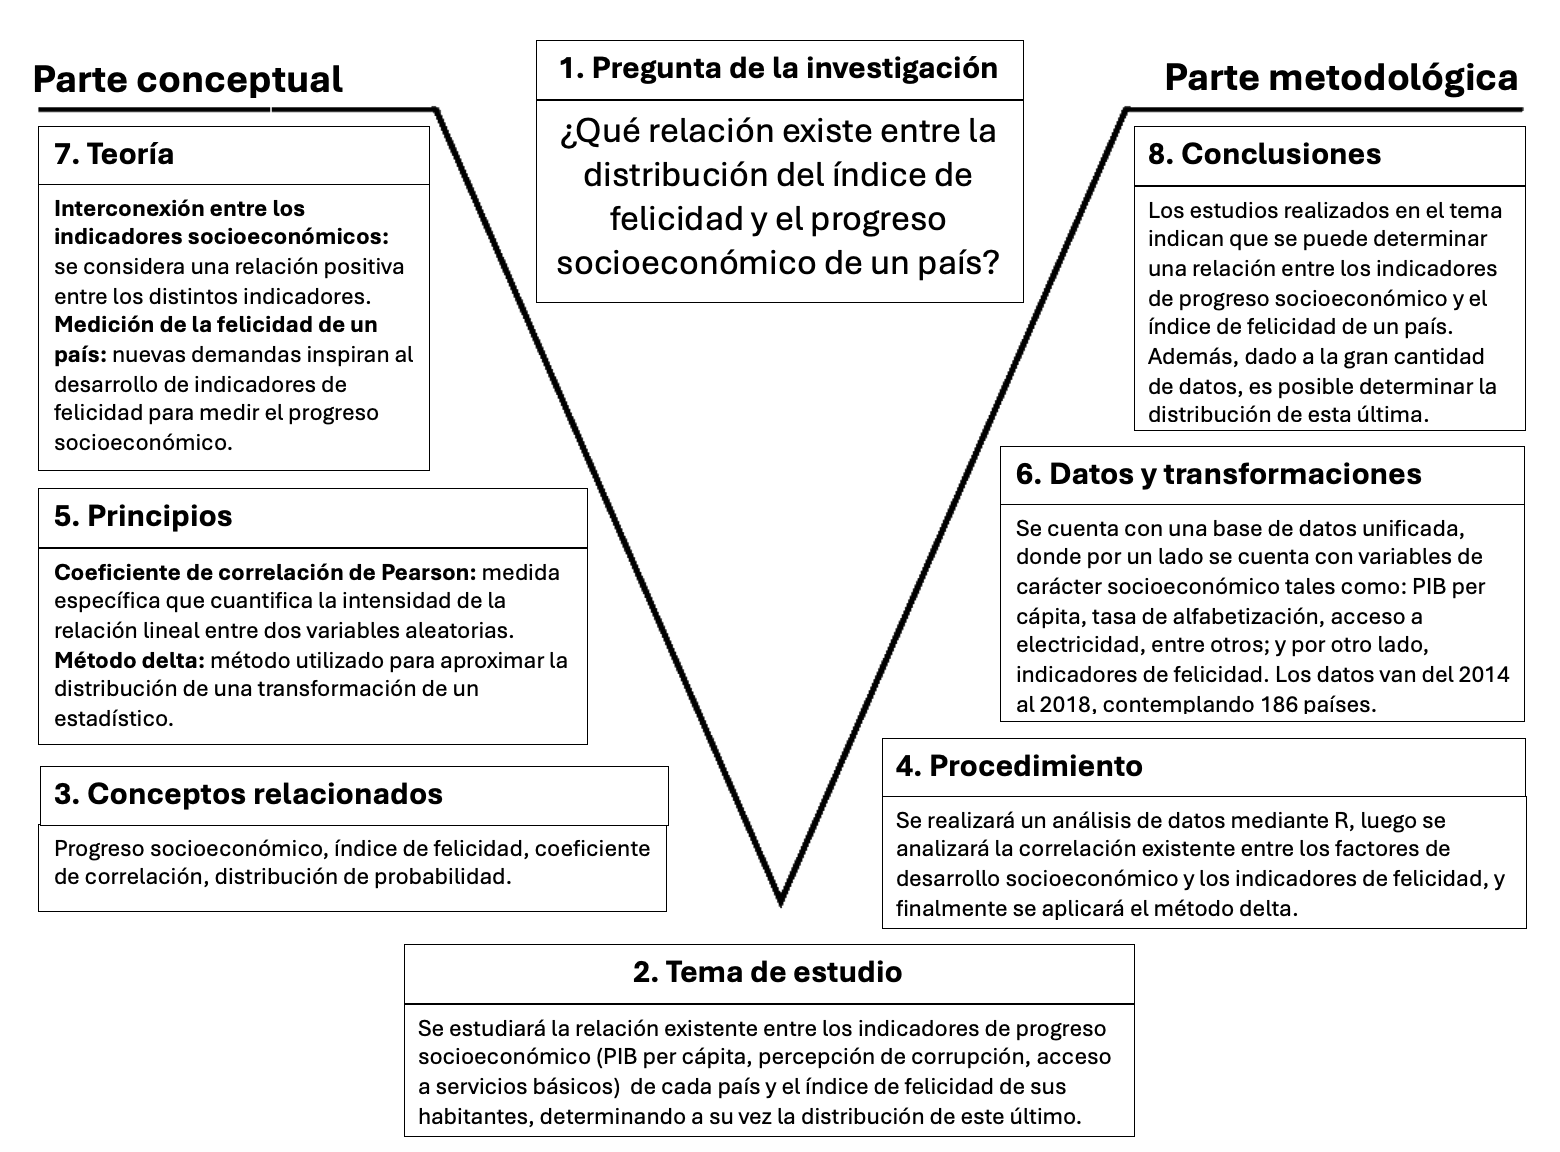
\includegraphics[width = 17cm]{figures/diagrama_uve2.png}
    \end{figure}

\newpage

\section{Parte de escritura}
\textbf{¿Qué relación existe entre la distribución del Índice de Felicidad y el progreso económico de un país?} \\

La relación que existe entre el Índice de Felicidad y el progreso económico suele ser medida con respecto a distintas variables las cuales representan un alto grado de utilidad para la comprensión de cómo estas afectan a la felicidad que se experimenta en el país. Esto se presenta de interés para la toma de decisiones gubernamentales e implementación de políticas públicas, con el fin de mejorar la vida de los habitantes de un territorio y maximizar el bienestar social en este.\\
    
Los estudios actuales denotan la existencia de una relación entre la felicidad y el progreso económico, algunos de estos casos presentan un crecimiento de la felicidad de la cual se goza a medida que aumenta el ingreso, como lo es el caso de Perú de la forma en la que expresa Tinoco (2020). 
\begin{quote}
    Un punto interesante sobre el estudio de esta relación es que no parece existir un punto de saciedad, es decir, un umbral o nivel límite donde un mayor ingreso personal no propicie mayor felicidad. Los datos y estudios realizados refieren que la capacidad del ingreso de influir sobre el bienestar no tiene límites.
    \flushright (Tinoco, 2020) 
\end{quote}

En el caso de Perú, se observa una relación positiva entre el ingreso y la felicidad, a tal punto de que no se observa una cota superior en la capacidad del ingreso en su influencia hacia la felicidad.\\
    
Mientras que el caso contrario también se encuentra presente, el cual se resume en una disminución de la felicidad a pesar de un aumento de variables económicas, como es el caso de Bután:  ``De hecho, la correlación, en este caso negativa, es bastante elevada; del -71 \% en términos absolutos. Ha habido un crecimiento económico, no obstante no ha aumentado la satisfacción a nivel general'' (Aguilar, et al., 2015). Un aumento de factores económicos presentó un efecto contradictorio en Bután durante el periodo del 2006-2009 con respecto al fenómeno observado en Uruguay.\\

Estos dos comportamientos se encuentran presentes a lo largo de los territorios que conforman las naciones, por lo cual se ha establecido como tarea principal, realizar un análisis de los datos recopilados de los distintos países, así como estudiar la correlación que existe entre las distintas variables presentes que funcionan como métricas del progreso económico y la felicidad. ``El estudio de la relación entre la felicidad y variables económicas como el ingreso, el desempleo y la inflación; este tipo de investigación ha generado una abundante XV.'' (Tinoco, 2020) Relacionar la felicidad con distintas variables económicas es un proceso que se ha llevado a cabo de forma abundante en distintos países.\\
    
Además de realizar el análisis de datos y correlación entre las distintas variables, se busca identificar las variables de mayor relevancia para este índice, para así poder desarrollar intervalos de confianza, y a su vez aproximar la distribución que siguen las distintas variables económicas con respecto a la felicidad.

\begin{quote}
    El intervalo de confianza describe la variabilidad entre la medida obtenida en un estudio y la medida real de la población (el valor real). Corresponde a un rango de valores, cuya distribución es normal y en el cual se encuentra, con alta probabilidad, el valor real de una determinada variable. Esta «alta probabilidad» se ha establecido por consenso en 95\%.
    \flushright (Candia, 2005)
\end{quote}

Esto con el fin de establecer un intervalo de confianza con respecto a los índices de correlación obtenidos para las distintas variables. Esto con la intención de obtener una mayor comprensión acerca de la correlación existente, dando lugar a resultados con una base más sólida. \\

Finalmente se va a encontrar la distribución que presenta la variable de la felicidad ya que tanto la composición de esta como su relación con distintas variables económicas presenta una naturaleza compleja. Se desea hallar la distribución con el fin de presentar información mas completa y estructurada. Además de que se presenta una mayor facilidad a la hora de identificar patrones y la forma en la que se relacionan distintas variables.\\

El estudio de análisis de datos y correlación que se desea llevar a cabo se presenta como un problema complejo debido a las distintas formas que pueden influir las variables en la felicidad de un territorio en especifico, por lo cual es de suma importancia el llevar a cabo un trabajo ordenado y estructurado, que tome en cuenta intervalos de confianza que permitan estimar la variabilidad presente, y la naturaleza de las distribución de la felicidad para tener una visión más completa.
% --- Bitácora 2 ---
\chapter{Bitácora 2} \label{bitacora2}
Las correcciones realizadas de la Bitácora 1 y las sugerencias se detallan en los Apéndices [\ref{Apendices}], mientras que los cambios fueron realizados propiamente en la Bitácora 1 [\ref{bitacora1}].
\section{Parte de planificación}

\subsection{Ordenamiento de la literatura}

\begin{table}[!h]
    \begin{center}
        \begin{tabular}{| m{2.5cm} | m{2.7cm} | m{3cm} | m{3cm} | m{1cm} | m{2.5cm} |}
        \hline\textbf{Tipo} & \textbf{Tema General} & \textbf{Tema Específico}& \textbf{Título} & \textbf{Año} & \textbf{Autor(es)}\\ \hline
        Metodológica & Correlación y Análisis de datos & Relevancia del Índice de felicidad & Crecimiento económico, progreso social y felicidad & 2017 & Luisa Montuschi\\ \hline
        Metodológica & Correlación y Análisis de datos & Relación felicidad-salud & Salud y Felicidad en Uruguay & 2010 & Mariana Gerstenblüth, Todd Jewell y Máximo Rossi \\ \hline
        Metodológica & Correlación y Análisis de datos &  Relación felicidad-progreso & ¿Suponen las directrices politicoeconómicas del Reino de Bután,... & 2014-2015 & Ignacio Aguilar, Oriol-Jordi Andrés, Guillem Foucault, et al.\\ \hline
        Metodológica & Correlación y Análisis de datos & Relación movilidad social-felicidad & Movilidad social, preferencias redistributivas y felicidad en Colombia. & 2011 & Juliana Londoño Vélez\\ \hline
        \end{tabular}
    \end{center}
\end{table}

\newpage
\section{Enlaces de la literatura}
En orden según la sección anterior, se dan los enlaces de las literaturas. \\

En el siglo XXI, se ha cuestionado la capacidad del Producto Interno Bruto (PIB) para medir adecuadamente el progreso social, dando lugar al desarrollo de nuevos indicadores como el Social Progress Index y el Gross National Happiness Index. Estos indicadores emergentes buscan superar las limitaciones del PIB al abordar aspectos más amplios del bienestar y la felicidad de la sociedad. La organización Social Progress Imperative ha liderado esfuerzos para crear el Social Progress Index, mientras que el Gross National Happiness Index, publicado anualmente desde 2012 en el World Happiness Report, también ha ganado reconocimiento.\\

\textbf{Resumen:} Lograr que el Producto Interno Bruto (PIB) mida correctamente el progreso social es un gran cuestionamiento ante la relevancia del índice con la realidad vivida por la sociedad. En un país centrado en el progreso, es importante abarcar todo lo posible sobre la realidad humana,  lograr cuantificarlo, y así dando un mejor resultado en el futuro. Por ello, se han creado varios índices sociales, como el Social Progress Index y el Gross National Happiness Index para lograr comparar e inclusive superar las limitaciones de los índices de progreso económico, como tiene el Producto Interno Bruto, y así no solo tomar en cuenta un progreso económico que puede ser muy centralizado, si no observar un muestreo de la realidad de las personas con características sociales. \\

\textbf{Contraste:} Por otro lado, últimamente se han sufrido varios eventos catastróficos, uno de estos es la pandemia del Covid-19, que han hecho a los países contemplar aun más la situación de sus habitantes. En sí, ``La pandemia puso al descubierto la vulnerabilidad de las sociedades y resaltó la interconexión entre factores sociales, naturales y económicos.'' (Alkire, 2023). Poner en alarma a la población de los países hace analizar datos vitales como los de este estudio.\\

\textbf{Contribución propia:} La reflexión sobre la necesidad de ir más allá del Producto Interno Bruto (PIB) para medir el progreso social es crucial en un mundo de constante cambio y enfrentando desafíos globales como lo fue la pandemia del Covid-19. La crisis sanitaria ha puesto resaltado la importancia de considerar no solo los aspectos económicos, sino también los sociales, para comprender verdaderamente el bienestar de las sociedades. \\

El estudio analiza la relación que existe entre el estado de salud y felicidad auto percibida, en el territorio de Uruguay a lo largo del año 2008. Se asocia el hecho de gozar de un buen estado de salud con un nivel mas alto de felicidad, siendo este a su vez, uno de los mayores determinantes de la felicidad. Se realiza un estudio además de diversas variables como lo son: desempleo, completación de la educación terciaria, religiosidad, así como factores socioeconomicos con la felicidad. Se estudia la influencia que puede representar la endogeneidad para encontrar una relación con respecto a la felicidad. Finalmente se concluye con la importancia que representa el estado de salud con respecto a la felicidad en Uruguay. \\

En el caso de Uruguay, el estudio busca concentrar la investigación entre la relación que se desarrolla entre la felicidad personal y la auto-percepción del estado de salud, utilizando la encuesta Religión, Salud y Emancipación Juvenil del ISSP para Uruguay en el 2008. Del estudio se obtiene que la salud es la variable que presenta la mayor relación con respecto a la felicidad. Para evitar problemas de heterogeneidad observable que se pueda desarrollar en dicha variable, se realizan estimaciones utilizando métodos pertinentes. Estos resultados se ven respaldados por estudios realizados en la misma región con anterioridad obteniendo resultados similares\\

\textbf{Resumen:} El estudio busca encontrar la relación existente entre la salud y la felicidad en Uruguay, se trata como variable dependiente a la felicidad, la cual se observa como una variable binaria, en la cual el individuo se reporta como feliz o no. Debido a la dificultad que presentan los problemas de endogeneidad se busca utilizar métodos adecuados para establecer las relaciones, uno de los utilizados es el \textit{propensity score}, lo cual busca un control de variables socioeconómicos para estimar el efecto que presenta la salud directamente en la felicidad, además de utilizarse métodos de relación como \textit{nearest neighbors}, Kernel y estratificación, así como \textit{Average Treatment effect on the Treated}. De forma resumida, el estudio busca la relación que existe entre diversos factores, enfocados en la salud, con respecto a la felicidad y a su vez utilizando métodos para reducir los posibles sesgos debido a la naturaleza de los datos.\\

\textbf{Contraste:} De la misma forma que concluye Amado Peiró (2001) en Condiciones Socioeconomicas y Felicidad de los Españoles, la salud resulta ser un factor sumamente importante para determinar la felicidad, la relación que presenta resulta intuitiva y corresponde de forma positiva con una multitud de estudios realizados con anterioridad, mientras que otras variables presentan una relación menor o casi inexistente, la salud se observa con una relación fundamental con respecto a la felicidad, ya sea en territorios de América Latina, como se expone en el estudio de Gerstenbluth, así como en territorios Europeos.\\

\textbf{Contribución propia: }Se observa en base a las relaciones obtenidas tanto en España como en Uruguay que la salud sobresale como un factor crítico para determinar la felicidad personal. Se observa que el bienestar físico y mental están fuertemente relacionados con la felicidad. Ambos estudios buscan tratar de forma adecuada los problemas de endogeneidad y sesgos en la estimación de efectos causales, para esto se utilizan métodos como el \textit{propensity score} y técnicas de correspondencia. La evidencia del análisis posterior demuestra la relevancia que presenta la salud como uno de los determinantes más importantes de la felicidad en distintos contextos territoriales. Políticas y programas impulsados por el gobierno tienen el potencial de generar un impacto significativo en la felicidad de las distintas poblaciones, los resultados pueden ser de interés para el diseño de políticas públicas y estrategias gubernamentales.\\

Bután tuvo un crecimiento económico bastante significativo entre los años 1980-2013, espacio en que se realiza el análisis. Esta economía se destaca entre sus vecinos, inclusive teniendo el segundo crecimiento más alto en todo el mundo por un momento. Además, la felicidad interna bruta (FIB) de Bután también destaca. La investigación intenta hacer una correlación entre las variables para intentar postular a la economía dada como ejemplar, y dado esto logra intuir que, por ejemplo, una gran riqueza no implica una felicidad más grande. El estudio compara con Nepal, Bangladesh, en métodos cercanos porque son economías similares, y también con economías grandes, donde se logra ver que Bután se comporta en correlación de manera distinta al mundo, donde entre más crecimiento económico se logre, más alto es el Índice de Felicidad.\\

\textbf{Resumen:} El estudio comienza intentando enfatizar la relevancia de la felicidad, en especial en el caso específico de Bután. Denota que la orientación popular es concentrarse en el Producto Interno Bruto, indicador del progreso económico muy central en los países, cuando dejan de lado lo que puede ser la felicidad de la sociedad. Dentro del estudio se logra ver algunos índices de diferentes países para poder contrastarlo con el caso de Bután. Dentro de este, se utilizan diferentes gráficos y correlaciones para lograr distinguir los diferentes países, así igual de manera conjunta, donde se exponen varios países y el mundo. La investigación trata comprender la correlación positiva de Bután entre los indicadores del Producto Interno Bruto y la Felicidad Interna Bruta, y lo compara con el resto del mundo, viendo cierto patrón a tener una correlación negativa. También trae al caso a Nepal y Bangladesh, para tratar de hacer la comparación más cercana. Sus gráficos y análisis le permite hacer la conclusión de que, aunque significativo progreso económico en los países en las últimas décadas, no se ha visto la misma fuerza en la felicidad, e intenta enfocar que se debería seguir como marco de ejemplo el caso de Bután. \\

\textbf{Contraste:} Sin embargo, como lo trabaja Abraham Aparicio Cabrera (2019) con \textit{Economía y Felicidad}, la economía de la felicidad es una rama importante de la economía, proponiendo el ingreso y consumo como variables relevantes y bases del bienestar general de las personas. ``Aunque la economía de la felicidad es un campo muy activo en las últimas tres décadas, algunos autores creen que es exagerado hablar de una disciplina subalterna de la economía'', en especial si estamos tratando de relacionar ambas variables principales por fuera del marco teórico, sino del práctico. Aparicio procede a encontrar diferentes percepciones de la felicidad, y subdividirlas, entre sacrificio y esfuerzo, con placer y dinero; que podemos observar como la satisfacción social y económica. Si bien es cierto que la felicidad cuenta con gran relevancia de la felicidad al menos subjetivamente, este estudio enfoca que hay una leve división en la relación de las variables. \\

\textbf{Contribución propia:} El caso de Bután es bastante particular ya que no sigue el patrón mundial, mostrando ambos indicadores de progreso económico y felicidad subir conjuntamente. Si bien es cierto que el muestreo son pocos años para llegar a una conclusión certera, al menos en el corto plazo se logra distinguir que el resto del mundo no sigue la misma línea que Bután. La subjetividad de la felicidad es bastante relevante también en casos de estudio como estos, pues los datos pueden estar sesgados localmente ante un concepto de felicidad percibido, donde por ejemplo un país desarrollado intenta de buscar un progreso social mientras la felicidad en otros países más bien yace en poder organizar bien los materiales económicos. Por eso tratar con temas como la economía de la felicidad y la leve división de la felicidad como diferentes percepciones es crucial para el comprendimiento de una satisfacción social \\

El estudio busca relacionar los determinantes de ingreso, movilidad social e injusticia social con el nivel de felicidad de sus habitantes, tratando de hacer un empate entre los resultados empíricos del estudio con las observaciones teóricas que han tenido otros contemporáneos. El estudio logra el objetivo de validar algunas observaciones teóricas, pero contradiciendo otras, además de encontrar que el nivel de ingreso si motiva a la felicidad, pero que no influye en las políticas de redistribución de la riqueza. \\

\textbf{Resumen:} El estudio de Londoño buscaba buscar una relación entre los determinantes de movilidad social, ingreso y justicia social con la felicidad y la demanda de redistribución. Donde las conclusiones finales de este estudio se pueden resumir en tres puntos, el primero es que las personas del estudio resultaron ser pesimistas en cuanto a su experiencia en la movilidad, pero que tenían buenas perspectivas de sus hijos para que ellos si tuvieran más movilidad social. Luego el otro hallazgo es que las personas de mayor ingreso tienen más felicidad que las personas de menor ingreso. Y como último punto, el ingreso resulta ser un determinante pobre de la demanda de redistribución, es decir, que no necesariamente las personas de ingresos más altos quieren una economía libre. \\

\textbf{Contraste:} El trabajo hace un desarrollo exhaustivo por dejar claro qué son todas las variables que va a tomar en cuenta, también indica la importancia que tiene una buena definición de felicidad para poder tratarla desde un punto de vista económico, ya que se llega a la conclusión de que aunque hay relación positiva ingreso-felicidad, sigue siendo muy débil y que tratar un concepto tan amplio como la felicidad desde una rama del conocimiento no es lo óptimo, pues al ser un concepto tan grande, necesita que haya un trabajo interdisciplinario para poder abordarla con mayor detalle y precisión. \\

\textbf{Contribución propia:} Como podemos observar ambos estudios tiene un enfoque de determinar si la felicidad se ve afectada por ciertos factores, en este caso, uno que tienen en común es el ingreso y hacen buenas acotaciones extras de ciertos resultados. Para llevar un orden, ambos estudios comienzan el análisis definiendo qué se entiende por felicidad, cómo se analiza y desde qué punto de vista lo harán, aunque ambos estudios lo hacen desde el punto de vista económico, dejan muy en claro al lector que este concepto va más allá de un punto de vista económico, pues es un término que ha intentado ser definido desde la filosofía y psicología, hasta últimamente en la economía. \\

Ambos estudios suponen que la felicidad viene dada por una utilidad, y bien ambas mencionan que esta es una falencia que tienen ambos estudios, pues hay otros factores que afectan enormemente a la felicidad, como lo son la cultura de país, por ejemplo. Luego cada uno va a utilizar una metodología diferente, donde el estudio de Londoño se hace una revisión bibliográfica, análisis de datos y un trabajo de campo para poder tener más información, el estudio de Álvarez lo hace desde una fuerte revisión bibliográfica y análisis de datos, sin presentar un trabajo de campo, sin embargo, en el estado del arte de cada uno de estos trabajos, hay muchas referencias donde tienen estudios con otro tipo de metodologías y que al final llegan a conclusiones igual o muy similares, lo que hace que se refuercen entre ellas y agregando información adicional, que también refuerza, en el estudio actual respectivo. \\

Antes de seguir, es importante mencionar la paradoja de Easterlin, el cual fue pionero en definir la felicidad desde el punto de vista económico, haciendo uso de la función de utilidad para ello, esta paradoja lo que indica es que a mayores niveles de ingreso menor es el aumento en la felicidad, lo que es lo mismo que hay una Utilidad Marginal Decreciente. Ambos estudios parten de esta idea, pues nace la pregunta ¿Qué tanto impacto hay dado tales factores? Tanto el estudio de Londoño, como el estudio de Álvarez llegan a la conclusión de que hay una relación positiva entre ingreso y felicidad de las personas, aunque también hacen el hincapié de que esta relación es muy débil, pues estamos delimitando el concepto de felicidad a una sola área que vendría siendo la económica.\\



\newpage

\subsection{Fichas nuevas de literatura}
\begin{table}[!ht]
    \caption{Ficha de Literatura 5}
    \begin{center}
        \begin{tabular}{  m{3cm} | m{12cm}  }
        \hline\textbf{ Encabezado} & \textbf{Contenido }\\ \hline
        Título: & Economía de la felicidad: Incidencia de los cambios de las variables macroeconómicas sobre la felicidad de los habitantes de américa latina. \\ \hline
        Autor(es): & Daniela Álvarez Zuluaga \& Caroline Londoño Díez  \\ \hline
        Año: & 2016 \\ \hline
        Nombre del tema: & Relación entre felicidad, ingreso, PIB, ICTR y Balanza Comercial. \\ \hline
        Cronológica: &  2003-2016 \\ \hline
        Metodológica: & Metodología de carácter cuantitativo y va a ser desarrollada a través de un modelo de panel de datos, el cual será de tipo estático. \\ \hline
        Temática: & Estudios económicos y psicológicos \\  \hline
        Teórica: & Economía de la felicidad. \\ \hline
        Resumen en una oración: & Qué factor afecta más a la felicidad dado el PIB, inflación, ITCR y BC. \\ \hline
        Argumento central: &  Determinar cómo los factores mencionados afectan a la felicidad \\ \hline
        Problemas con el argumento o el tema: & No toma en cuenta el desempleo que sería un factor muy considerable a tener en cuenta. Además, es un estudio de análisis y revisión bibliográfica, no hubo trabajo de campo, porque está tratando con datos anteriores e información que posiblemente ya ha cambiado. \\ \hline
        Resumen en un párrafo: & El ensayo hace un trabajo exhaustivo por dejar claro qué son todas las variables que va a tomar en cuenta, también indica la importancia que tiene una buena definición de felicidad para poder tratarla desde un punto de vista económico, ya que se llega a la conclusión de que aunque hay relación positiva ingreso-felicidad, sigue siendo muy débil y que tratar un concepto tan amplio como la felicidad desde una rama del conocimiento no es lo óptimo, pues al ser un concepto tan grande, necesita que haya un trabajo interdisciplinario para poder abordarla con mayor detalle y precisión. \\ \hline
        \end{tabular}
    \end{center}
\end{table}

\begin{table}[H]
    \caption{Ficha de Literatura 6}
    \begin{center}
        \begin{tabular}{  m{3cm} | m{12cm}  }
        \hline\textbf{ Encabezado} & \textbf{Contenido }\\ \hline
        Título: &  Economía y felicidad: ¿Importa lo que las personas entienden por felicidad?\\ \hline
        Autor(es): & Abraham Aparicio Cabrera \\ \hline
        Año: &  2019\\ \hline
        Nombre del tema: & Conexión entre la felicidad y la economía \\ \hline
        Cronológica: & 2014 \\ \hline
        Metodológica: & Estudio de bases de datos de una encuesta. Contrastes, comparaciones y correlaciones  \\ \hline
        Temática: & Estudios económicos y psicológicos\\ \hline
        Teórica:  & Economía de la felicidad \\ \hline
        Resumen en una oración: & Los factores económicos son vitales a la hora de percibir la felicidad según las personas \\ \hline
        Argumento central: & Averiguar la relación entre la percepción de felicidad y los factores económicos \\ \hline
        Problemas con el argumento o el tema: & Como recalca el artículo, la felicidad puede ser algo subjetivo y difícil de cuantificar, en términos relativos con el progreso económico. Además, la muestra parece un poco localizada, por lo que los datos podrían estar sesgados a una sección local.  \\ \hline
        Resumen en un párrafo: & El estudio define por un lado la felicidad y la economía de la felicidad. Hace uso de una base de datos basada en la Encuesta Nacional de Satisfacción con la Vida y la Sociedad, creada por la Universidad Nacional Autónoma de México. En este, encuentra varias conexiones y datos que destacan en las creencias populares de las personas, pero solo se visualizan porcentajes y no muestras agrupadas, como para poder comparar los grupos varios de diferentes ingresos. También destaca la felicidad como placer y dinero, o la felicidad como sacrificio y esfuerzo, al lograr encontrar grandes cantidades de observaciones que se inclinaban a alguna de las dos.   \\ \hline
        \end{tabular}
    \end{center}
\end{table}

\begin{table}[H]
    \caption{Ficha de Literatura 7}
    \begin{center}
        \begin{tabular}{  m{3cm} | m{12cm}  }
        \hline\textbf{ Encabezado} & \textbf{Contenido }\\ \hline
        Título: &  Condiciones Socioeconomicas y
        Felicidad de los Españoles
        \\ \hline
        Autor(es): & Amado Peiró \\ \hline
        Año: &  2001\\ \hline
        Nombre del tema: & Conexión entre la felicidad y condiciones socioeconomicas \\ \hline
        Cronológica: & 1995 \\ \hline
        Metodológica: & Estudio de bases de dato de una encuesta. Contrastes, comparaciones y correlaciones  \\ \hline
        Temática: & Estudios económicos y psicológicos\\ \hline
        Teórica:  & Economía de la felicidad \\ \hline
        Resumen en una oración: & Encontrar una aproximación de la relación entre condiciones socio económicas y felicidad desde la evidencia disponible en España. \\ \hline
        Argumento central: & Impacto de las condiciones socio económicas con respecto a la felicidad desde la evidencia disponible en España\\ \hline
        Problemas con el argumento o el tema: & El estudio establece la felicidad como una variable compleja que requiere un acercamiento no únicamente desde un punto de vista económico, sino que la observa como una variable compleja que requiere un estudio tanto psicológico como sociológico  \\ \hline
        Resumen en un párrafo: & Inicialmente se describen las limitaciones presentes del estudio de la felicidad al tratarse de una variable compleja con elementos no únicamente económicos sino psicológicos y sociológicos. Seguido de esto se procede a explicar la base de datos a estudiar, la cual corresponde a los obtenidos de la Encuesta Mundial de Valores, la cual se realizó en España en 1995. Se establecen los principales factores ligados a la felicidad, estableciendo relaciones bivariadas con respecto a la felicidad, además se establecen tablas adecuadas acerca de las relaciones encontradas. Finalmente se reporta los hallazgos encontrados, se concluye que tanto la salud como la edad representan una fuerte relación con la felicidad de los individuos. \\ \hline
        \end{tabular}
    \end{center}
\end{table}

\begin{table}[H]
    \caption{Ficha de Literatura 8}
    \begin{center}
        \begin{tabular}{  m{3cm} | m{12cm}  }
        \hline\textbf{ Encabezado} & \textbf{Contenido }\\ \hline
        Título: &  Lecture Notes on Asymptotic Statistics \\ \hline
        Autor(es): & Changliang Zou \\ \hline
        Año: &  2014\\ \hline
        Nombre del tema: &  Transformaciones de estadísticos: El método Delta\\ \hline
        Cronológica: &  N.A. \\ \hline
        Metodológica: & Método Delta \\  \hline
        Teórica: &  Transformaciones de estadísticos\\ \hline
        Resumen en una oración: &  Aplicaciones del método delta para obtener la distribución de las transformaciones de estadísticos. \\ \hline
        Argumento central: &  Lo esencial de este documento es el ejemplo 2.4.2. ya que sirve de guía para unir la correlación con la aproximación de la distribución de una variable. \\ \hline
        Problemas con el argumento o el tema: &  De momento no se puede determinar de manera concreta los problemas con el argumento ya que únicamente se está estableciendo la base de la idea a seguir. En el peor de los casos, el peor problema sería que no funcione para lo que se espera.\\ \hline
        Resumen en un párrafo: & Este documento con alta rigurosidad matemática se puede ver como una guía con metodologías estadísticas que se pueden llevar a cabo para diferentes aplicaciones. De momento nos vamos a enfocar en la sección con la información del método delta, el cual nos permitirá aproximar la distribución de dado parámetro, por medio de aplicaciones que se le pueden realizar a las transformaciones de los estadísticos.\\ \hline
        \end{tabular}
    \end{center}
\end{table}

\newpage

\section{Análisis estadísticos}
\subsection{Análisis descriptivo}

Para el set de datos a utilizar se decide reemplazar los valores N/A presentes en distintas entradas por el promedio de la variable en cuestión. La existencia de valores N/A es debido a que no todos los países reportan todos los años a las tres entidades de las cuales se obtienen los datos, esto debido a las distintas dinámicas geo-socio-políticas que se desarrollan en las distintas divisiones geográficas del mundo, así como la calidad de las relaciones que existe entre los países, o situaciones de guerra o crisis.

En la estructura que presentan los datos se puede observar que cada variable va en una columna, no existe una combinación de distintas variables en la misma columna. A su vez cada observación es única y sus valores están distribuidos a lo largo de una única fila, debido a la estructura que traía la base de datos no fue necesario el uso de funciones como pivot\_longer o pivot\_wider. Existe un identificador o key claro para cada una de las entradas, en este caso corresponde a la columna ``country'' que indica el país. Además, queremos que todas las variables manejen valores numéricos, así que se va a reemplazar los valores de ``income\_class'' por su factor, para de esta forma tener únicamente variables numéricas, y no se presentan valores N/A en ninguna entrada debido a que anteriormente se solucionó este problema.

Al respetarse las características anteriores podemos asegurar que la forma actual que presentan los datos se encuentran de la forma ``tidy'', la tabla se encuentra lista para realizar el análisis de datos exploratorio descriptivo

Ahora lo que vamos a realizar es un análisis descriptivo completo de la tabla. La forma más sencilla de empezar este proceso es mediante la función ``descr'', la cual permite obtener distintos estadísticos de la tabla en cuestión. Se procede a utilizar dicha función y se obtiene la tabla siguiente. Se decide transponer y seccionar la tabla debido a limitaciones de espacio.




\newpage

\begin{table}[!ht]
\caption{Estadísticas descriptivas de la base de datos}
\scriptsize
    \centering
    \begin{tabular}{|l|l|l|l|l|l|l|l|}
    \hline
         Variables & Mean & Std.Dev & Min & Q1 & Median & Q3 & Max \\ \hline
        adult\_literacy & 81 & 16 & 24 & 81 & 82 & 94 & 100 \\ \hline
        air\_pollution & 89 & 27 & 0 & 98 & 100 & 100 & 100 \\ \hline
        alcohol\_consumption & 6 & 4 & 0 & 2 & 5 & 9 & 17 \\ \hline
        cpi & 43 & 20 & 9 & 30 & 38 & 57 & 89 \\ \hline
        electricity\_access & 83 & 27 & 5 & 75 & 100 & 100 & 100 \\ \hline
        freedom\_to\_make\_life\_choices & 1 & 0 & 0 & 1 & 1 & 1 & 1 \\ \hline
        gdp & 519e9 & 1962e9 & 1e9 & 15e9 & 549e9 & 320e9 & 19228e9 \\ \hline
        gdp\_capita & 14338 & 20030 & 252 & 1573 & 5317 & 16660 & 109835 \\ \hline
        generosity & 0 & 0 & 0 & 0 & 0 & 0 & 1 \\ \hline
        healthy\_life\_expectancy\_at\_birth & 63 & 7 & 43 & 59 & 65 & 68 & 74 \\ \hline
        income\_class & 2 & 1 & 0 & 1 & 2 & 3 & 3 \\ \hline
        labor\_force & 21826609 & 77389989 & 202458 & 2080011 & 4774402 & 13210888 & 779046779 \\ \hline
        labor\_rate & 61 & 10 & 34 & 55 & 61 & 66 & 87 \\ \hline
        land\_area & 830832 & 2076693 & 300 & 54390 & 215262 & 652230 & 16376870 \\ \hline
        life\_expectancy & 72 & 8 & 52 & 66 & 74 & 79 & 84 \\ \hline
        life\_ladder & 5 & 1 & 3 & 5 & 5 & 6 & 8 \\ \hline
        log\_gdp\_per\_capita & 9 & 1 & 7 & 8 & 9 & 10 & 12 \\ \hline
        negative\_affect & 0 & 0 & 0 & 0 & 0 & 0 & 1 \\ \hline
        perceptions\_of\_corruption & 1 & 0 & 0 & 1 & 1 & 1 & 1 \\ \hline
        population & 48627541 & 164074313 & 340594 & 4751112 & 10949187 & 33844343 & 1391656250 \\ \hline
        population\_density & 212 & 691 & 2 & 34 & 81 & 187 & 7874 \\ \hline
        positive\_affect & 1 & 0 & 0 & 1 & 1 & 1 & 1 \\ \hline
        social\_support & 1 & 0 & 0 & 1 & 1 & 1 & 1 \\ \hline
        unemployment\_rate & 7 & 5 & 0 & 4 & 6 & 10 & 24 \\ \hline
        water\_access & 87 & 16 & 41 & 80 & 94 & 99 & 100 \\ \hline
    \end{tabular}
\end{table}

\begin{table}[!ht]
\scriptsize
    \centering
    \begin{tabular}{|l|l|l|l|l|l|l|}
    \hline
        Variables & MAD & IQR & CV & Skewness & SE.Skewness & Kurtosis \\ \hline
        adult\_literacy & 13 & 13 & 0 & -1 & 0 & 2 \\ \hline
        air\_pollution & 0 & 2 & 0 & -3 & 0 & 5 \\ \hline
        alcohol\_consumption & 5 & 8 & 1 & 0 & 0 & -1 \\ \hline
        cpi & 16 & 27 & 0 & 1 & 0 & 0 \\ \hline
        electricity\_access & 1 & 24 & 0 & -1 & 0 & 1 \\ \hline
        freedom\_to\_make\_life\_choices & 0 & 0 & 0 & -1 & 0 & 0 \\ \hline
        gdp & 70723843167 & 301553258272 & 4 & 7 & 0 & 62 \\ \hline
        gdp\_capita & 6520 & 14991 & 1 & 2 & 0 & 4 \\ \hline
        generosity & 0 & 0 & -51 & 1 & 0 & 1 \\ \hline
        healthy\_life\_expectancy\_at\_birth & 7 & 10 & 0 & -1 & 0 & 0 \\ \hline
        income\_class & 1 & 2 & 1 & 0 & 0 & -1 \\ \hline
        labor\_force & 5596694 & 11105457 & 4 & 8 & 0 & 68 \\ \hline
        labor\_rate & 8 & 11 & 0 & 0 & 0 & 0 \\ \hline
        land\_area & 283652 & 592372 & 2 & 5 & 0 & 26 \\ \hline
        life\_expectancy & 9 & 13 & 0 & -1 & 0 & -1 \\ \hline
        life\_ladder & 1 & 2 & 0 & 0 & 0 & -1 \\ \hline
        log\_gdp\_per\_capita & 1 & 2 & 0 & 0 & 0 & -1 \\ \hline
        negative\_affect & 0 & 0 & 0 & 1 & 0 & 2 \\ \hline
        perceptions\_of\_corruption & 0 & 0 & 0 & -2 & 0 & 2 \\ \hline
        population & 12729275 & 28660786 & 3 & 7 & 0 & 55 \\ \hline
        population\_density & 84 & 143 & 3 & 10 & 0 & 101 \\ \hline
        positive\_affect & 0 & 0 & 0 & 0 & 0 & 0 \\ \hline
        social\_support & 0 & 0 & 0 & -1 & 0 & 1 \\ \hline
        unemployment\_rate & 3 & 6 & 1 & 1 & 0 & 1 \\ \hline
        water\_access & 9 & 19 & 0 & -1 & 0 & 1 \\ \hline
    \end{tabular}
\end{table}

\newpage






Una vez obtenidas los estadísticos descriptivos de cada variable, tenemos indicadores claros de su comportamiento, pero para el estudio que se desea desarrollar es necesario obtener a su vez, la forma en la que se relacionan las distintas variables entre ellas. Por lo que resulta sensato el obtener una matriz de correlación entre las distintas variables para tener índices normalizados que muestren la forma en la cual se comporta una variable con respecto a otra, pero la gran cantidad de variables presentes en la base de datos dificulta que se aprecie de forma adecuada la matriz, por lo que se utiliza un gráfico de correlación entre las variables.



\begin{figure}[!ht]
    \centering
    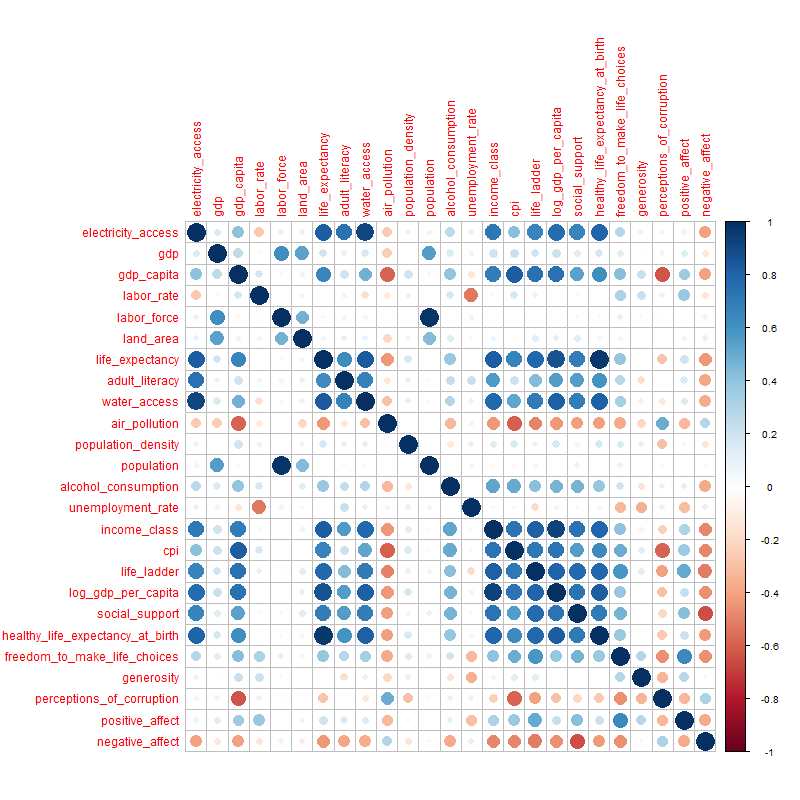
\includegraphics[width=0.9\textwidth]{figures/correlaciones.png}
    \caption{Tabla de correlaciones}
    \label{fig:correlaciones}
\end{figure}

\newpage

Del gráfico de correlación se logra observar de forma sencilla cuales son las variables que tienen una relación más fuerte con nuestra variable de estudio life\_ladder, las cuales corresponden a electricity\_access, gdp\_capita, life\_expectancy, water\_access, income\_class, cpi, log\_gdp\_per\_capita, social\_support, healthy\_life\_expectancy\_at\_birth, freedom\_to\_make\_life\_choices.

El presente estudio busca relacionar variables del progreso socioeconómico del país con respecto a life\_ladder, de forma que de las variables anteriormente mencionadas se decide tomar como variables relevantes las siguientes:
\begin{itemize}
    \item electricity\_access: El acceso de la población a la electricidad se observa como un factor importante en la promoción de la educación y la información, lo que tienen repercusión en la productividad de un territorio en especifico, además de que un índice mayor, representa el acceso en zonas rurales, lo cual se observa como catalizador de desarrollo económico.
    \item water\_access: El acceso de la población al agua potable se presente como factor fundamental en salud y bienestar, para ser mas específicos en seguridad alimentaria, lo cual es un factor fundamental no solo para el desarrollo económico sino para el funcionamiento integral de cualquier sociedad.
    \item income\_class: La clase social dominante en un territorio esta estrechamente ligada con respecto al progreso económico del país, una clase económica de un estrato superior esta relacionada con países primer mundistas, los cuales tienen un progreso económico mucho mayor al resto del mundo.
    \item cpi: El índice de percepción de corrupción, tiene una fuerte relación con los gobiernos de turno de las distintas naciones, los cuales tienen gran influencia en los mercados y permisos para el desarrollo económico presente en los países.
    \item log\_gdp\_per\_capita: El PIB per capita ha sido uno de los factores mas determinantes en el desarrollo económico, así como uno de los más utilizados debido a su relación significativa con la economía de un país. Se decidió utilizar la forma logarítmica de este, debido a que el Producto Interno Bruto normal presentaba valores de magnitudes exageradas en comparación a los valores presentes en las otras variables, resulta mas sensato trabajar con la versión logarítmica.
\end{itemize}

\newpage

\begin{table}[!ht]
\caption{Estadísticas descriptivas life\_ladder}
    \centering
    \begin{tabular}{|l|l|}
    \hline
        Medida & Valor \\ \hline
        Mínimo & 3.08446157 \\ \hline
        1° Cuartil & 4.511907876 \\ \hline
        Media & 5.378751576 \\ \hline
        Promedio & 5.402009419 \\ \hline
        3° Cuartil & 6.172229697 \\ \hline
        Máximo & 7.688531995 \\ \hline
        Desviación Estándar & 1.12103288 \\ \hline
    \end{tabular}
\end{table}

Se decide agregar la tabla de estadísticas descriptivas de life\_ladder debido a que se trata de la variable de estudio queremos dar énfasis en cuales son los estadísticos que podemos calcular para esta variable y ver las propiedades de ésta dados los datos que utilizamos para el estudio. \\

\begin{table}[!ht]
\caption{Estadísticas descriptivas log\_gdp\_per\_capita}
    \centering
    \begin{tabular}{|l|l|}
    \hline
        Medida & Valor \\ \hline
        Minimo & 6.607255936 \\ \hline
        1° Cuartil & 8.481270671 \\ \hline
        Media & 9.4914397 \\ \hline
        Promedio & 9.355072582 \\ \hline
        3° Cuartil & 10.28644955 \\ \hline
        Máximo & 11.64962649 \\ \hline
        Desviación Estándar & 1.204099118 \\ \hline
    \end{tabular}
\end{table}

A su vez se agregan las estadísticas descriptivas de log\_gdp\_per\_capita debido a que en la mayoría de estudios se ha utilizado el Producto Interno Bruto per-capita como una de las variables más influyentes cuando se realizan estudios concentrados en factores del área económica como lo es el progreso económico. Como vimos en las referencias bibliográficas que hemos utilizado en el estado del arte de este trabajo, estos estudios demostraron que siempre hay una correlación positiva entre ingreso, el cual casi siempre se toma como el PIB per-capita en dichos estudios, y felicidad. \\ 

\newpage

\begin{table}[!ht]
\caption{Estadísticas descriptivas de las variables relevantes}
\scriptsize
    \centering
    \begin{tabular}{|l|l|l|l|l|l|l|}
    \hline
        Medida & cpi & electricity\_access & income\_class & life\_ladder & log\_gdp\_per\_capita & water\_access \\ \hline
        Mean & 43.36 & 82.99 & 1.74 & 5.40 & 9.36 & 87.40 \\ \hline
        Std.Dev & 19.69 & 27.39 & 1.05 & 1.12 & 1.20 & 16.25 \\ \hline
        Min & 9.25 & 5.15 & 0.00 & 3.08 & 6.61 & 40.77 \\ \hline
        Q1 & 29.50 & 75.31 & 1.00 & 4.51 & 8.48 & 80.16 \\ \hline
        Median & 37.50 & 99.53 & 2.00 & 5.38 & 9.49 & 94.14 \\ \hline
        Q3 & 56.75 & 100.00 & 3.00 & 6.18 & 10.29 & 99.32 \\ \hline
        Max & 89.25 & 100.00 & 3.00 & 7.69 & 11.65 & 100.00 \\ \hline
        MAD & 15.75 & 0.70 & 1.48 & 1.22 & 1.38 & 8.53 \\ \hline
        IQR & 27.13 & 24.13 & 2.00 & 1.66 & 1.81 & 18.83 \\ \hline
        CV & 0.45 & 0.33 & 0.60 & 0.21 & 0.13 & 0.19 \\ \hline
        Skewness & 0.76 & -1.45 & -0.21 & 0.04 & -0.32 & -1.32 \\ \hline
        SE.Skewness & 0.20 & 0.20 & 0.20 & 0.20 & 0.20 & 0.20 \\ \hline
        Kurtosis & -0.39 & 0.66 & -1.21 & -0.77 & -0.84 & 0.52 \\ \hline
    \end{tabular}
\end{table}


Finalmente se agrega una tabla con estadísticas descriptivas del resto de variables incluyendo las dos anteriores, esto porque como vimos en la figura 2, que es la tabla de correlación, donde pudimos ver que las variables que tomamos para realizar el trabajo poseen una correlación positiva, por ello, creemos pertinente hacer una uso del análisis exploratorio de datos en estas variables, para tener más información acerca de cómo se comportan, dada nuestra base datos.



\begin{figure}[!ht]
    \centering
    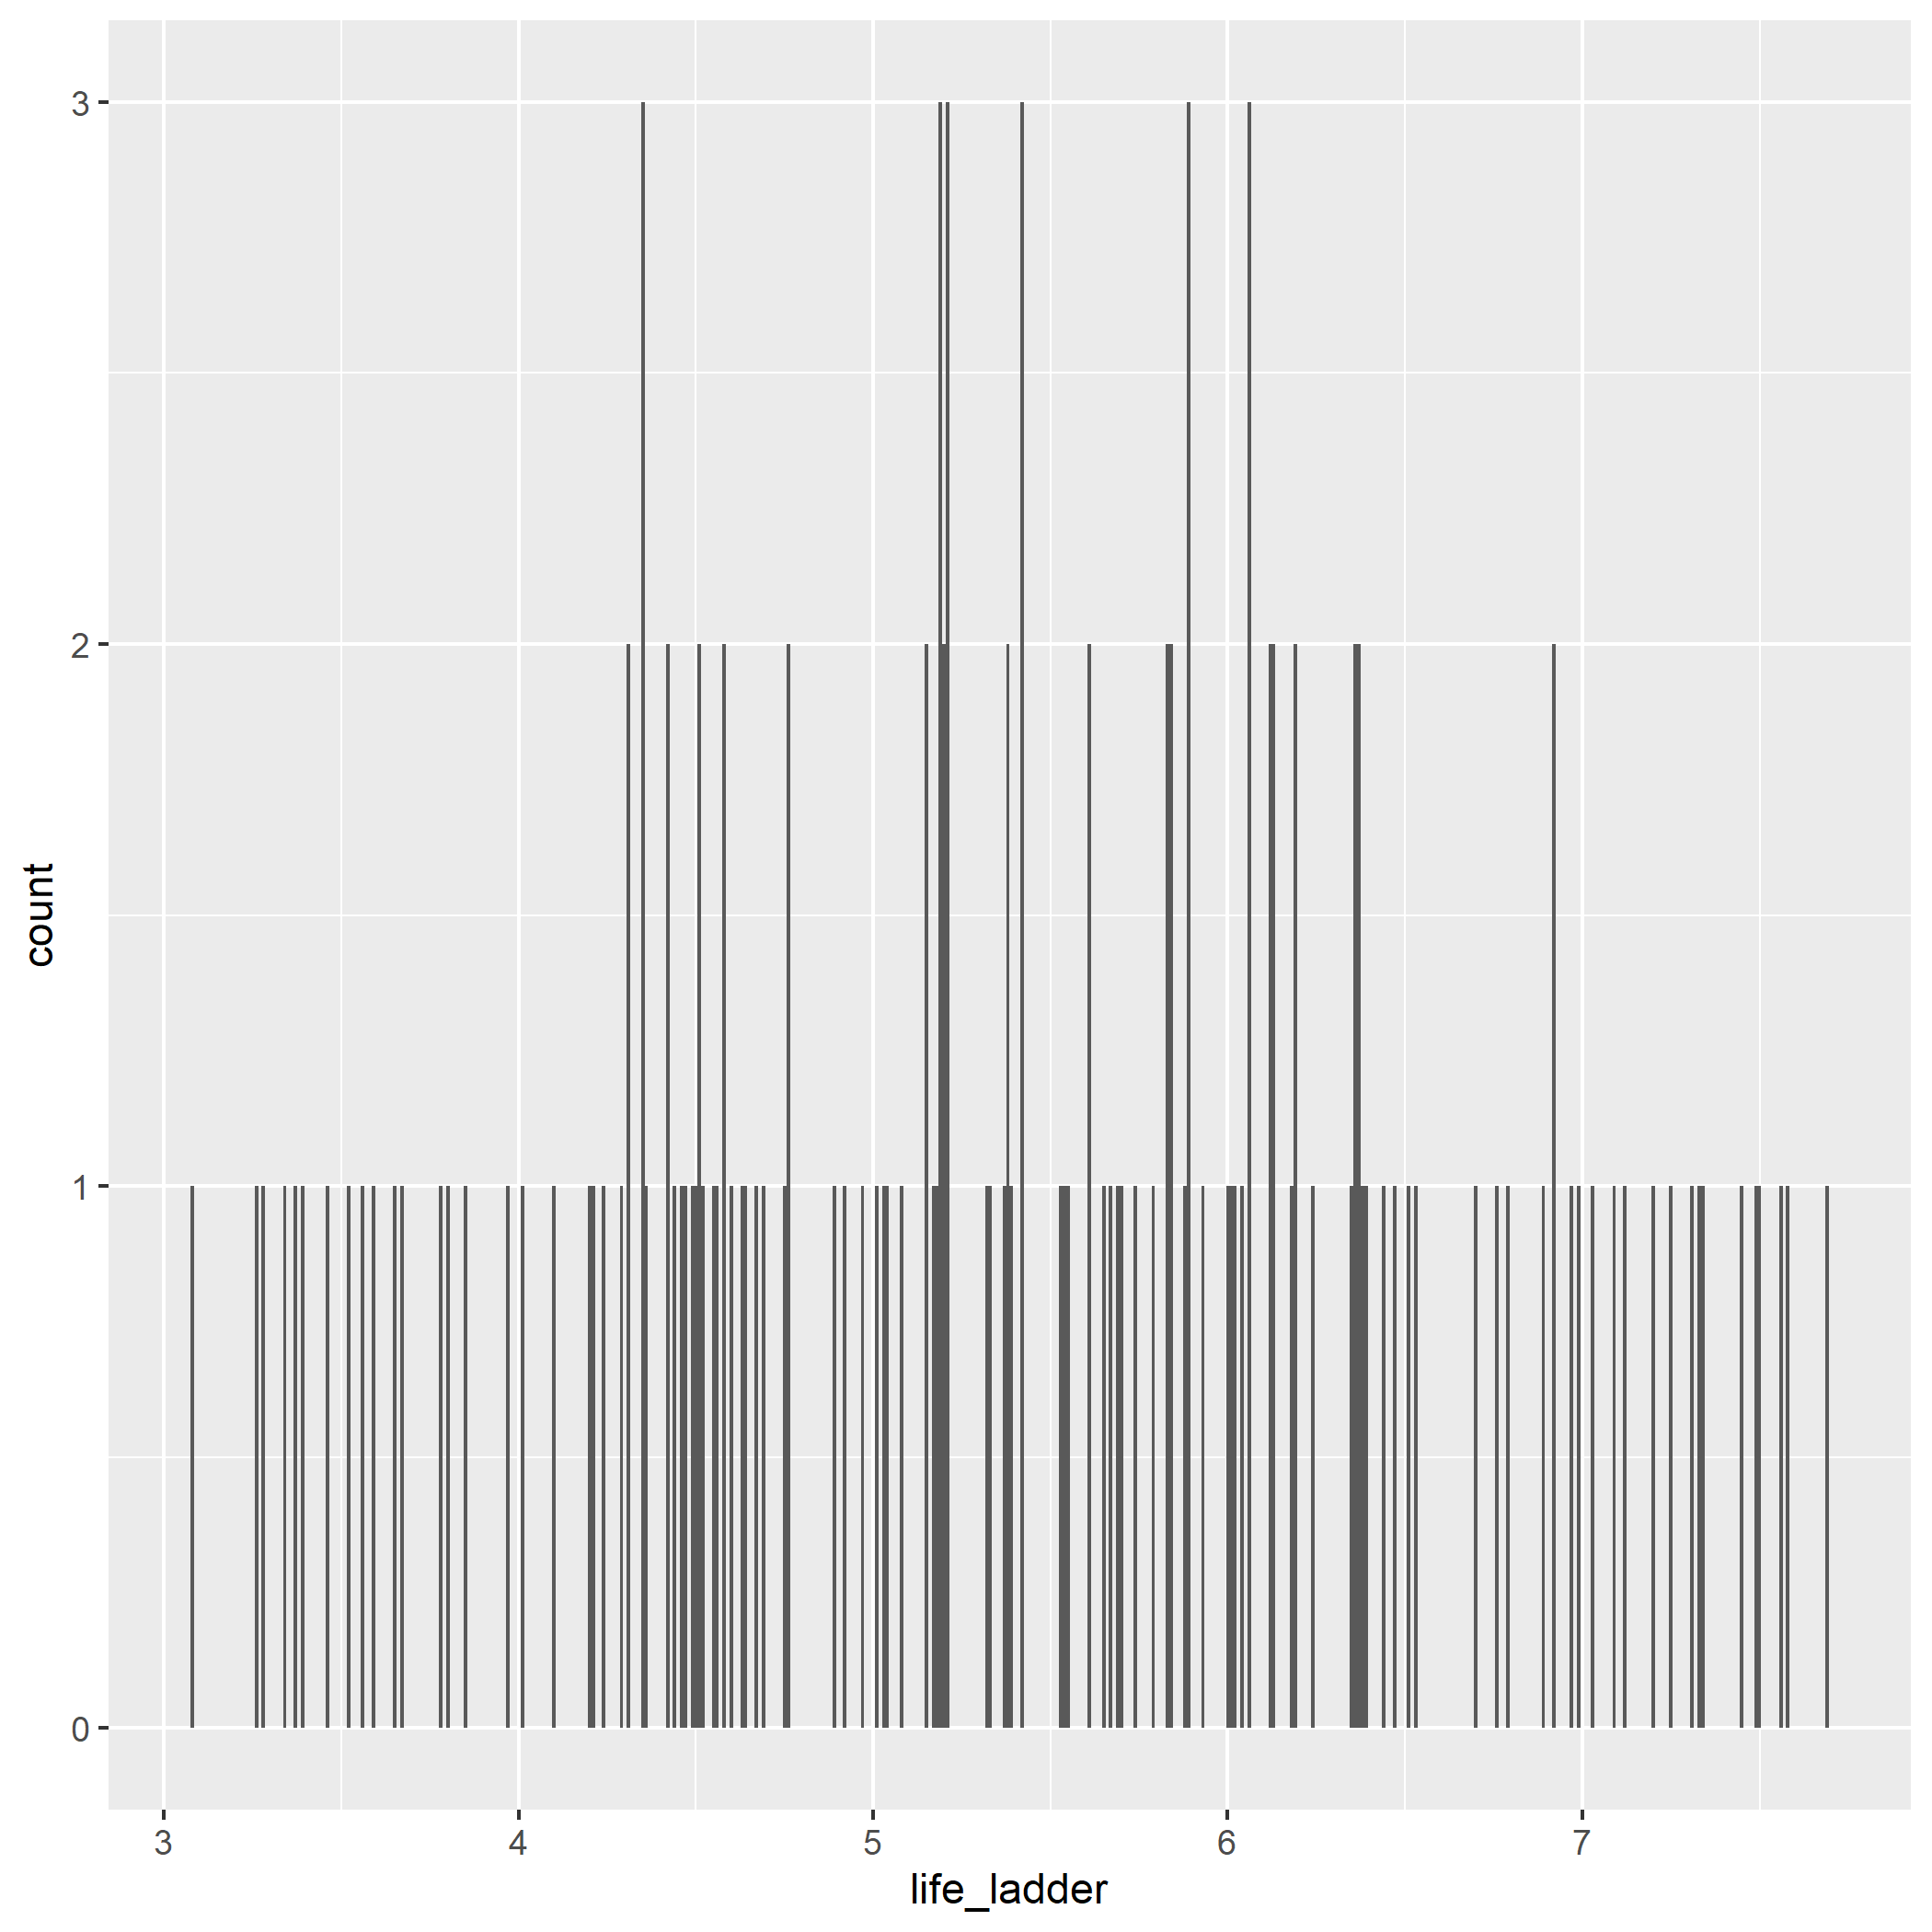
\includegraphics[width=0.3\textwidth]{figures/life_variacion.png}
    \caption{Comportamiento de life\_ladder}
    \label{fig:correlaciones1}
\end{figure}

El gráfico de Comportamiento de life\_ladder permite tener una visualización clara acerca de la distribución que presenta la variable principal, así como ser una herramienta útil para identificar la tendencia central por la cual se rigen estos datos, así como observar los datos atípicos. Aunque se tiene una tabla con las estadísticas descriptivas de la variable, resulta mucho mas intuitivo estudiar la data de una forma visual, en conjunto la tabla de variables descriptivas junto con el gráfico del comportamiento de life\_ladder se puede realizar un estudio completo de la variación de esta.
\newpage
\begin{figure}[!ht]
    \centering
    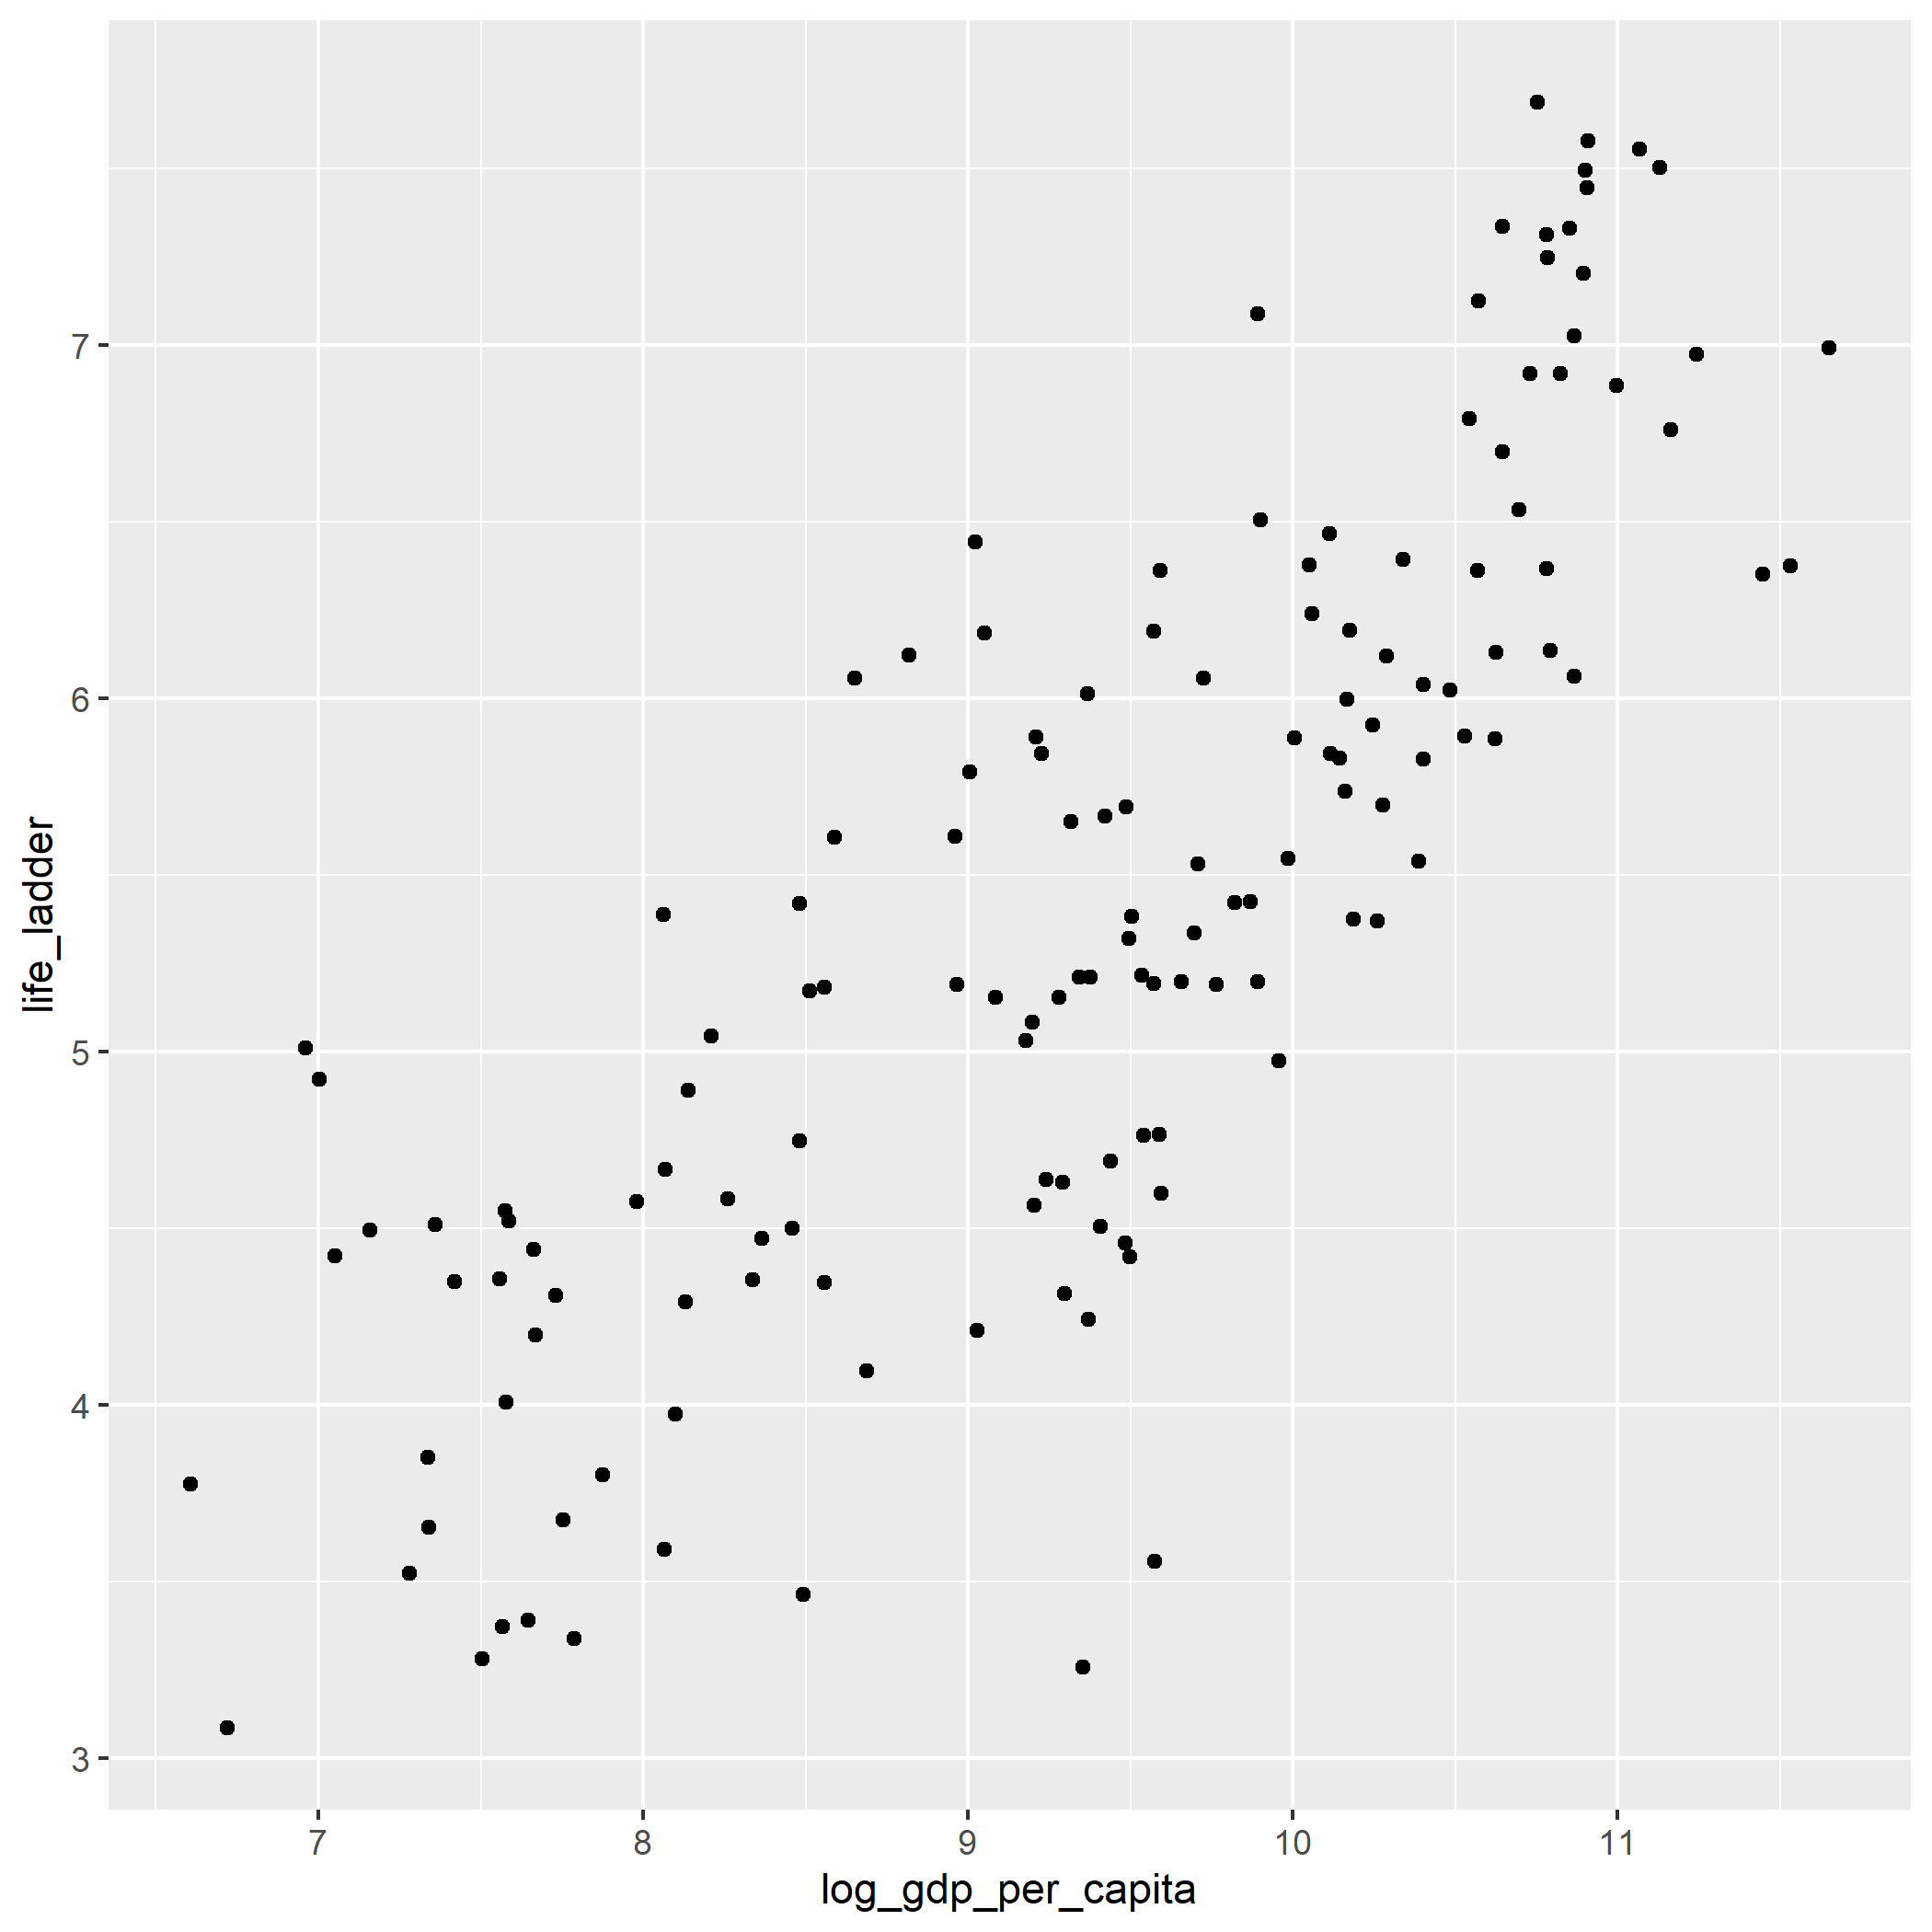
\includegraphics[width=0.3\textwidth]{figures/gdp_life.png}
    \caption{life\_ladder contra log\_gdp\_per\_capita}
    \label{fig:correlaciones2}
\end{figure}

El gdp\_per\_capita es una de las variables que presenta mayor relación con life\_ladder, el gráfico de estas dos variables nos permite apreciar de forma mas clara la relación positiva que existe entre estas dos, ya que el Producto Interno Bruto es uno de los componentes mas fundamentales para medir el progreso económico de una nación, obtener una relación positiva entre este y life\_ladder muestra un resultado favorecedor para la pregunta de investigación planteada, ya que se observa una clara relación positiva entre las variables.

\begin{figure}[!ht]
    \centering
    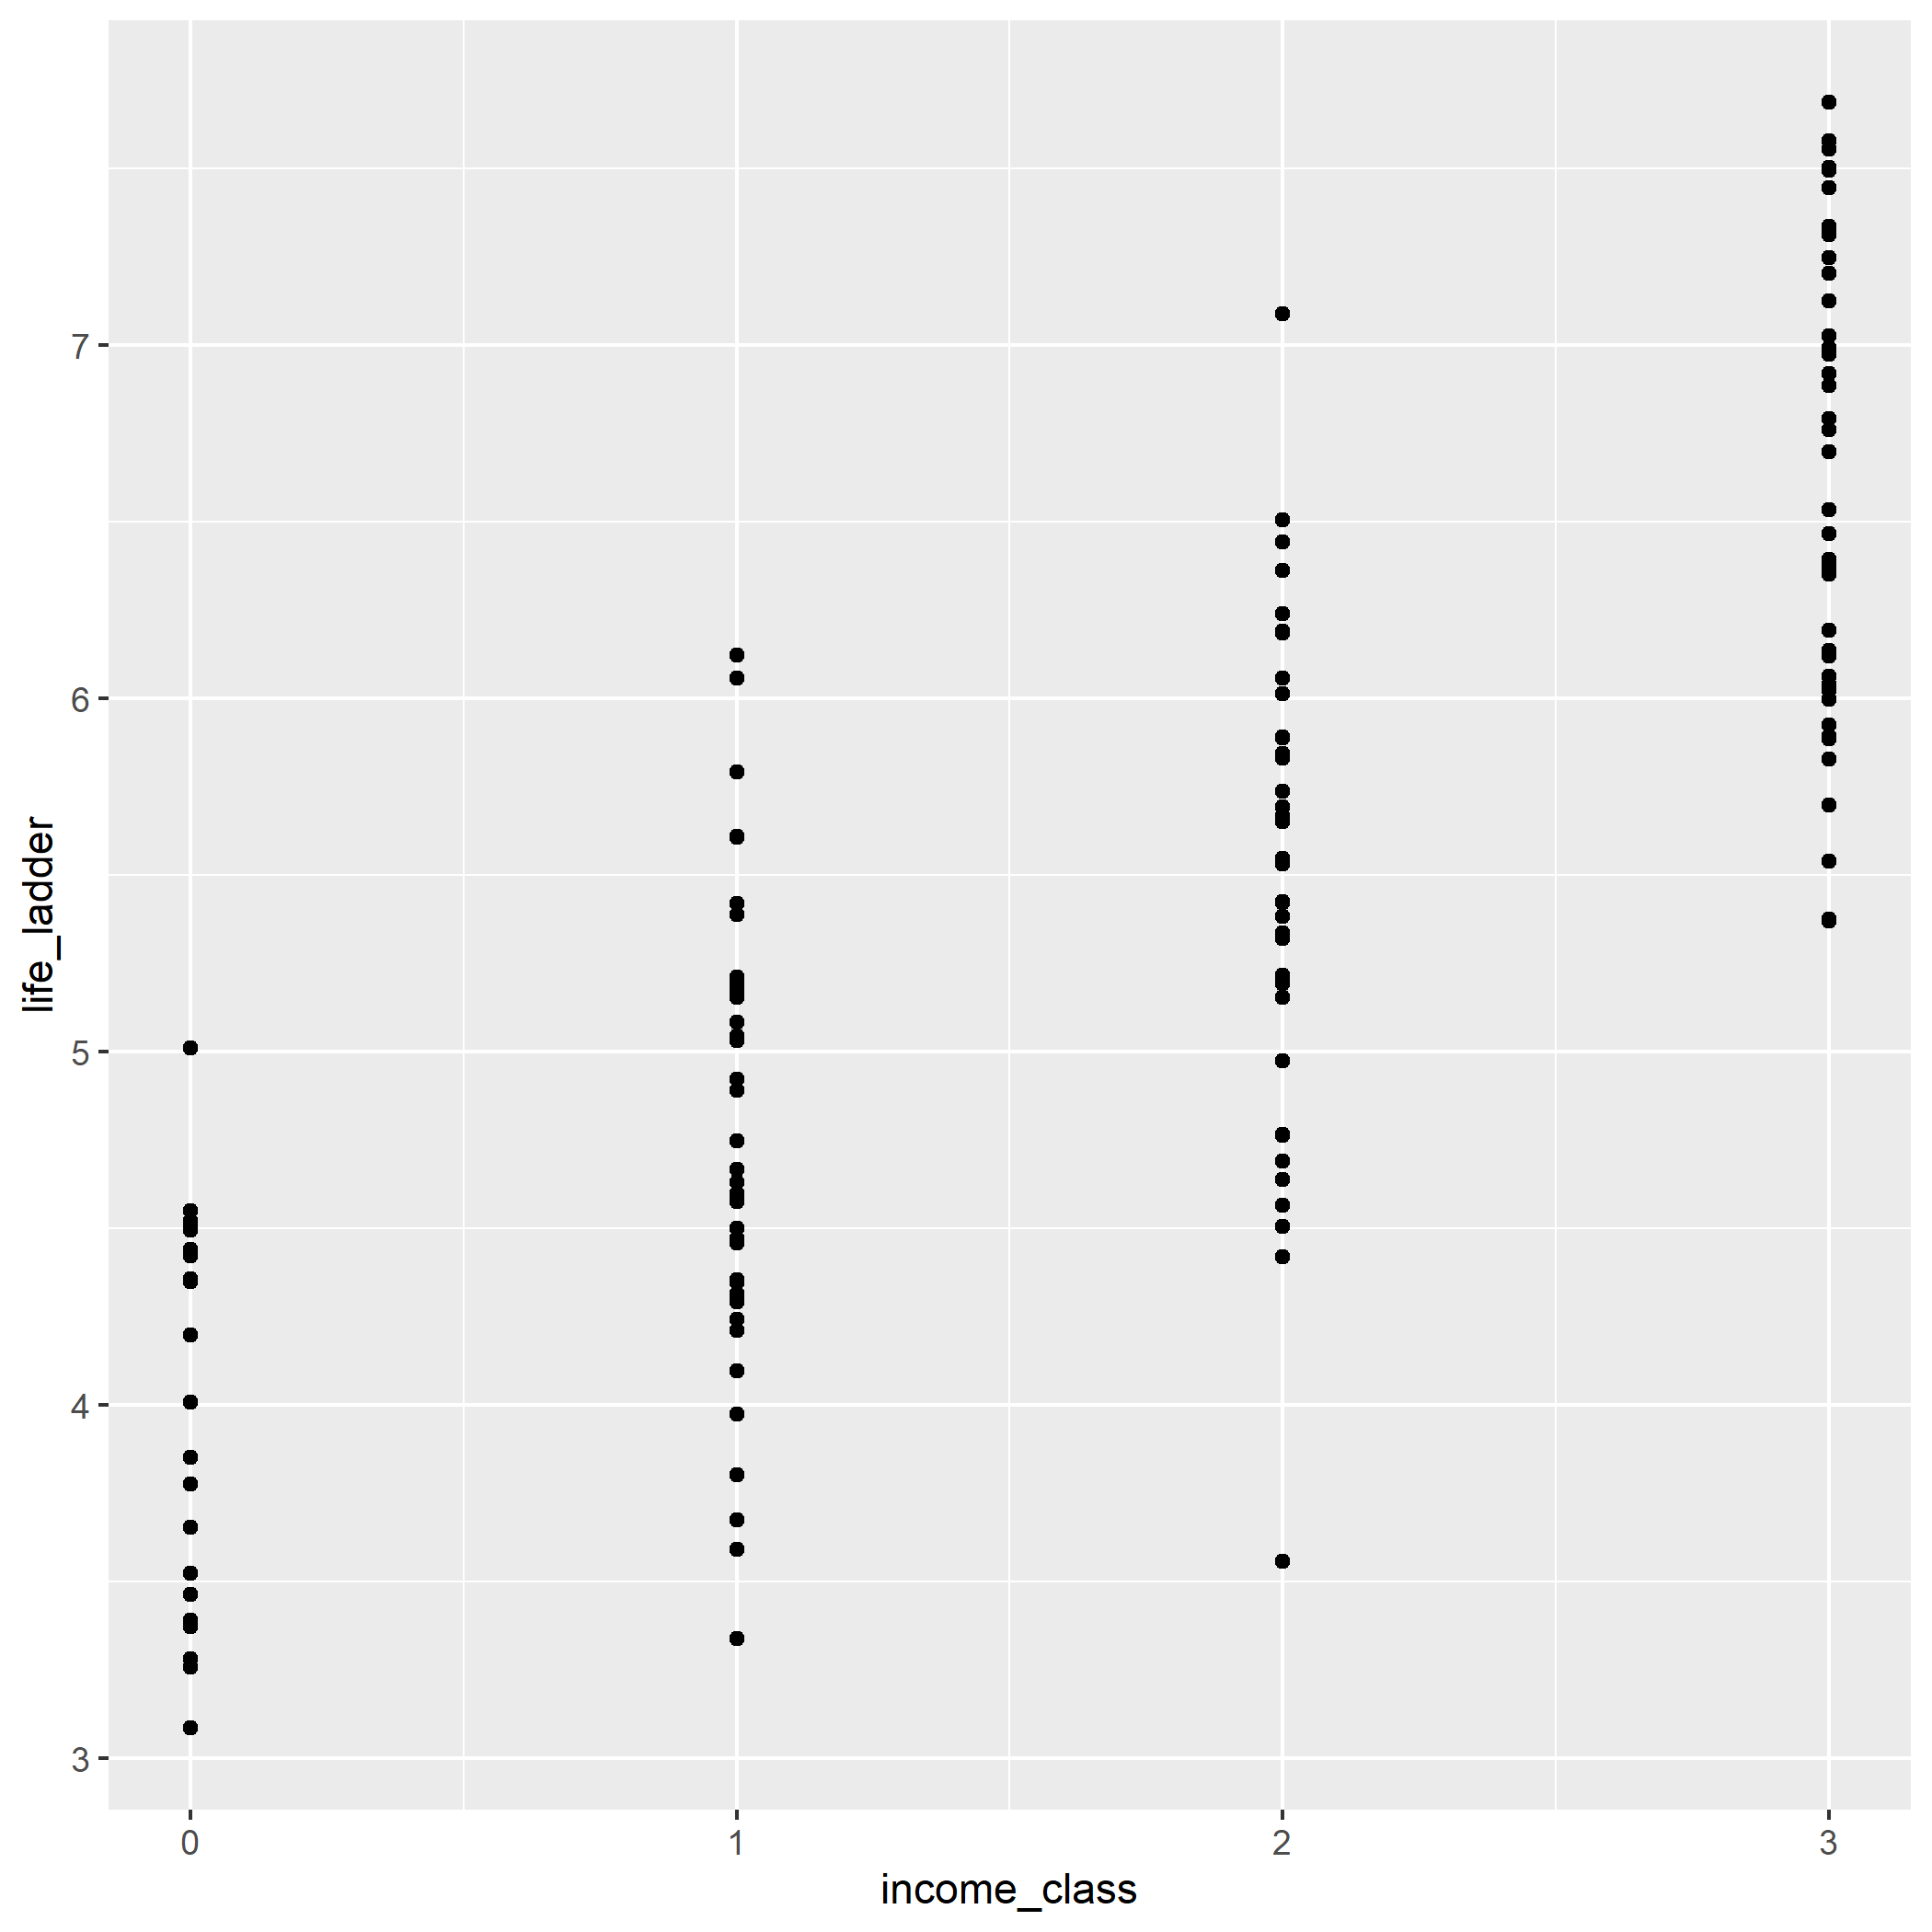
\includegraphics[width=0.3\textwidth]{figures/income_life.png}
    \caption{life\_ladder contra income\_class}
    \label{fig:correlaciones3}
\end{figure}

También se decide utilizar income\_class como una variable predicativa de life\_ladder, income\_class presenta el inconveniente de tratarse de una variable categórica, combinado con el hecho de que únicamente existen cuatro categorías, genera que esta variable no aporte tanta información como la pasada, pero se puede rescatar el hecho de que presentan una relación positiva y tanto máximos como mínimos de cada categoría tienen una magnitud mayor a las categorías anteriores, denotándose de esta forma una relación positiva entre las dos variables.

\newpage
\subsection{Propuesta metodológica}
La metodología escogida para llevar a cabo la tarea que se tiene puede dividirse en dos partes:

\begin{enumerate}
    \item \textbf{Coeficiente de correlación lineal de Pearson} \\
    El coeficiente de correlación de Pearson es un índice que mide el grado de variación entre distintas variables relacionadas linealmente. \\
    
    Supongamos que se tienen dos variables $X$, $Y$.
    Se define el coeficiente de correlación de Pearson entre estas dos variables como $r_{xy}$ entonces:
    \begin{equation*}
        -1 \leq r_{xy} \leq 1
    \end{equation*}

    Es importante mencionar que la magnitud de la relación vienen especificada por el valor numérico del coeficiente, mientras que el signo refleja la dirección de tal valor. \\

    Esto quiere decir que una relación de $+1$ es igual de fuerte a una relación $-1$, solamente cambia el sentido de esta.

   Una correlación positiva entre dos variables indica que a medida que una de ellas aumenta, la otra también lo hace. En el caso de que ambas aumenten en igual medida, se dice que son perfectamente positivas.

   De manera similar, una correlación negativa entre dos variables indica que a medida que una de ellas aumenta, la otra disminuye. En el caso de que ambas cambien en igual magnitud, se dice que son perfectamente negativas.

   El coeficiente de Pearson viene dado por la siguiente fórmula: \footnote{\cite{coef_pearsen}}
   \begin{equation}
       r_{xy} = \frac{\sum Z_x Z_y}{N} 
   \end{equation}
   
   Donde: 
   
   \begin{itemize}
       \item $Z_x$ es la desviación estándar de X
       \item $Z_y$ es la desviación estándar de Y
       \item N es la cantidad de datos 
   \end{itemize}

\newpage

\begin{lstlisting}[caption={Coeficiente de correlacion lineal de Pearson}, label=lst:rchunk1]
# Para obtener una visualizacion de data en ggplot2 mas eficiente
install.packages("ggpubr")
library("ggpubr")

# Obtenemos la correlacion utilizando distintos metodos, en este caso Pearson, Kendall y Spearman, vamos a concentrarnos en Pearson, pero los otros metodos nos permite tener una idea mas clara del comportamiento de los datos.
cor(x, y, method = c("pearson", "kendall", "spearman"))
cor.test(x, y, method=c("pearson", "kendall", "spearman"))

# Grafico de dispersion de la correlacion
ggscatter(Data_relevante, x = "life_ladder", y = "log_gdp_per_capita", 
          add = "reg.line", conf.int = TRUE, 
          cor.coef = TRUE, cor.method = "pearson",
          xlab = "Miles/(US) gallon", ylab = "Weight (1000 lbs)")

# Prueba de normalidad Shapiro-Wilk de las variables
shapiro.test(Data_relevante$life_ladder) 
shapiro.test(Data_relevante$log_gdp_per_capita)

# Inspeccion grafica de la normalidad de las variables
ggqqplot(Data_relevante$life_ladder, ylab = "life_ladder")
ggqqplot(Data_relevante$log_gdp_per_capita, ylab = "log_gdp_per_capita")

# Finalmente test de correlacion de Pearson
res <- cor.test(Data_relevante$log_gdp_per_capita, Data_relevante$life_ladder, 
                    method = "pearson")
res

# Interpretacion de resultados
# p.value: Valor p de la prueba
# estimate: coeficiente de correlacion
res$p.value
res$estimate
\end{lstlisting}
\newpage

\begin{figure}[!ht]
    \centering
    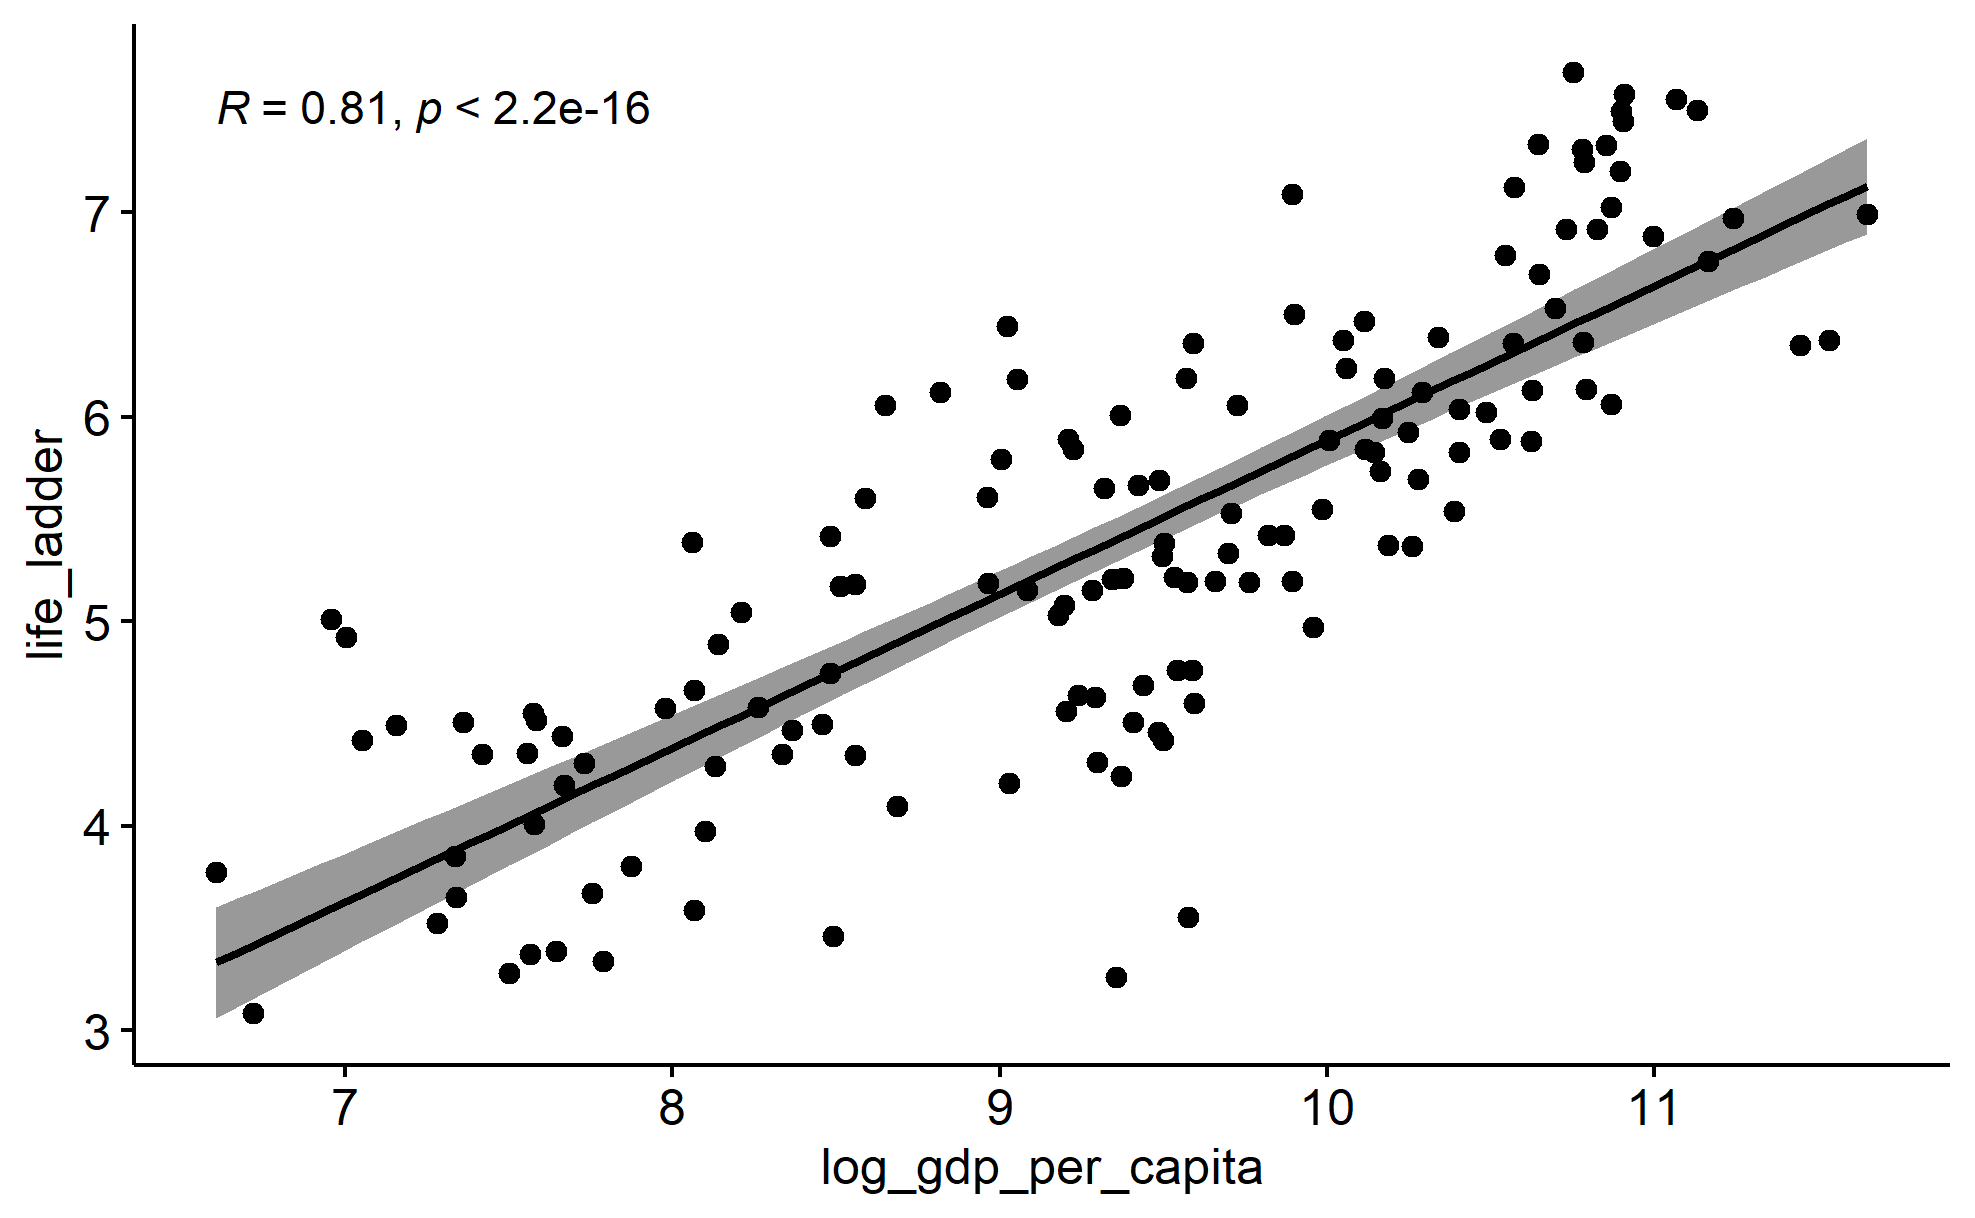
\includegraphics[width=0.5\textwidth]{figures/plot_Aa.png}
    \caption{life\_ladder contra log\_gdp\_per\_capita}
    \label{fig:correlaciones1}
\end{figure}

\begin{figure}[!ht]
    \centering
    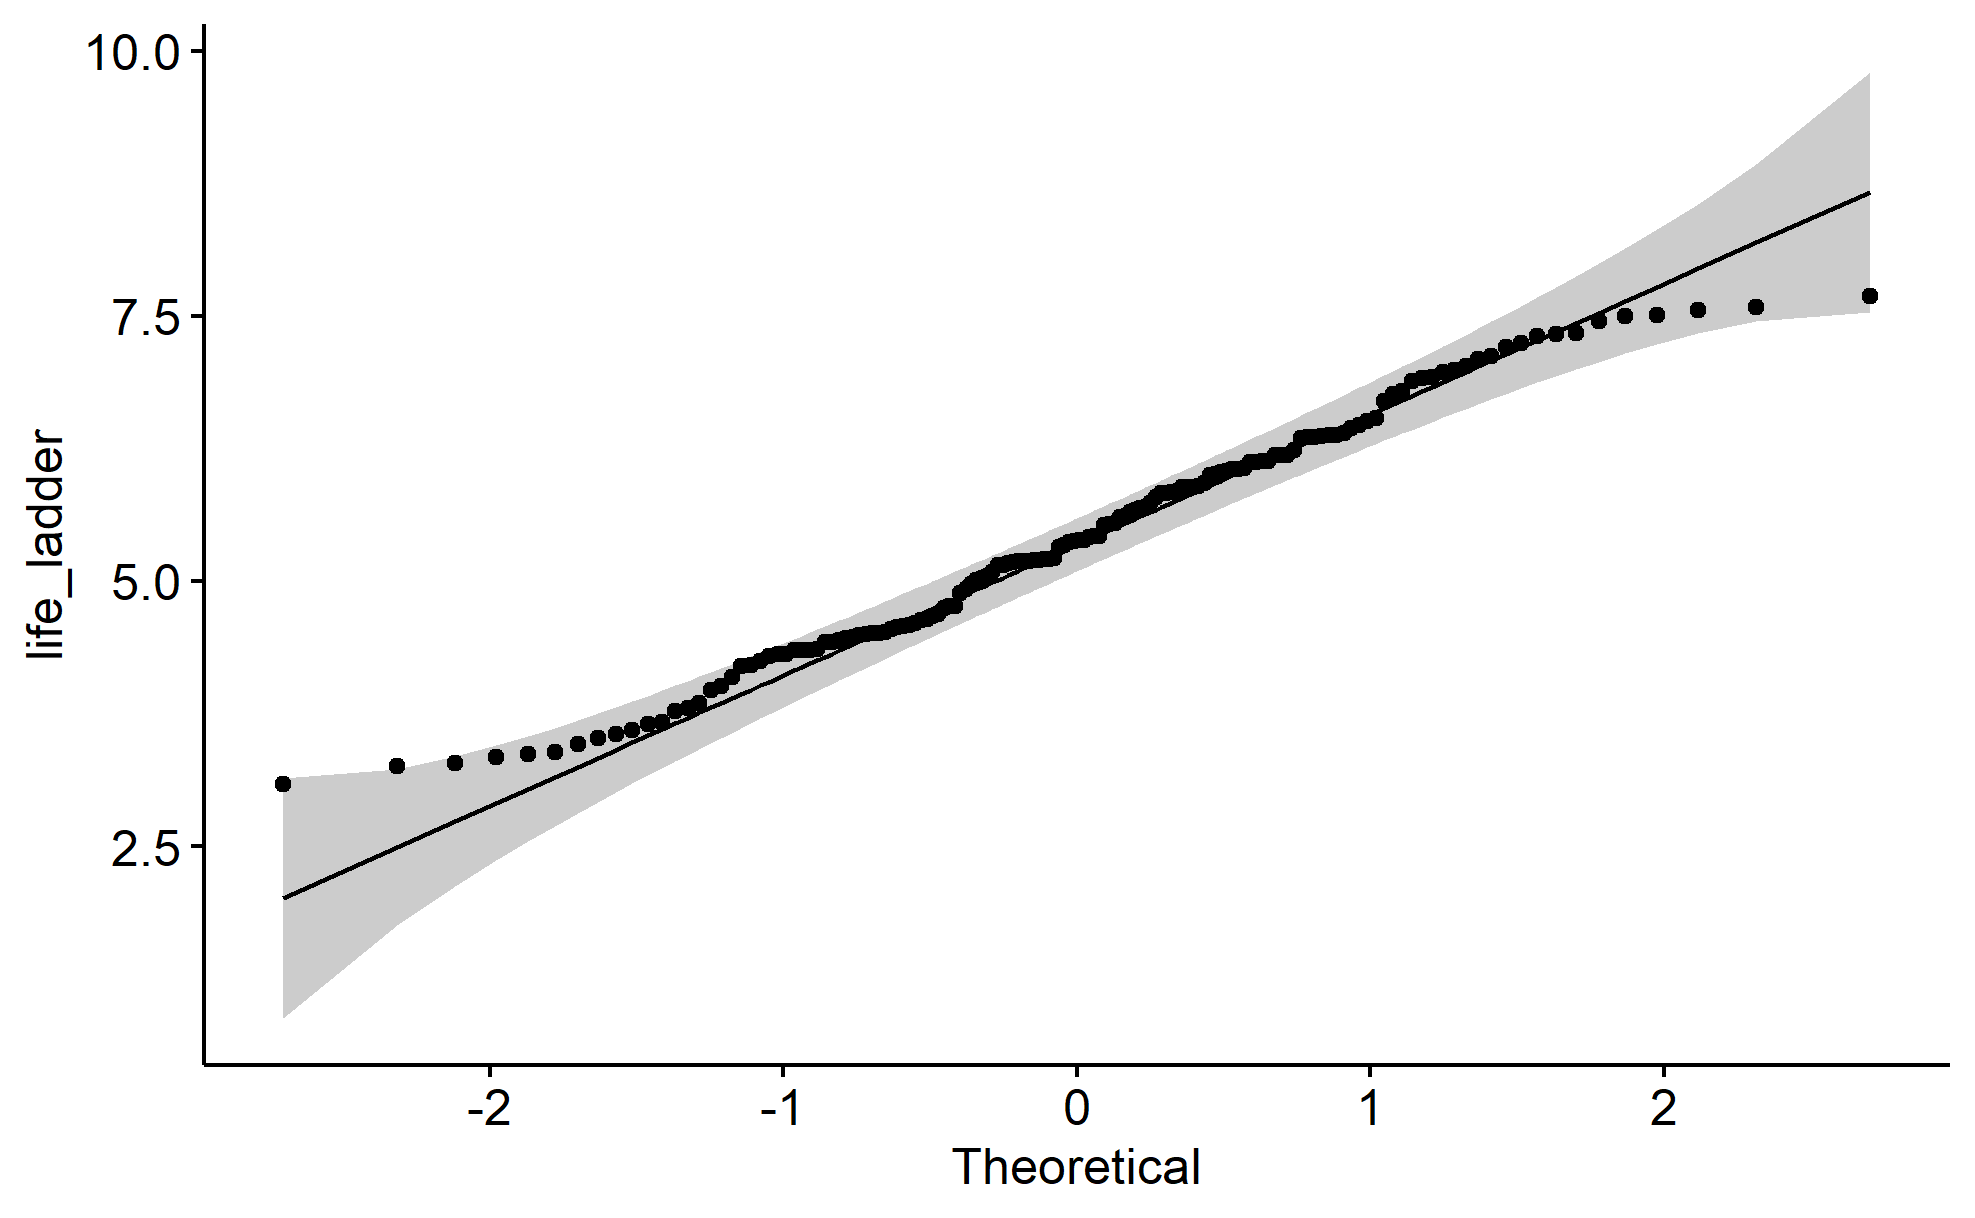
\includegraphics[width=0.5\textwidth]{figures/plot_Ab.png}
    \caption{Normalidad de life\_ladder}
    \label{fig:correlaciones2}
\end{figure}

\begin{figure}[!ht]
    \centering
    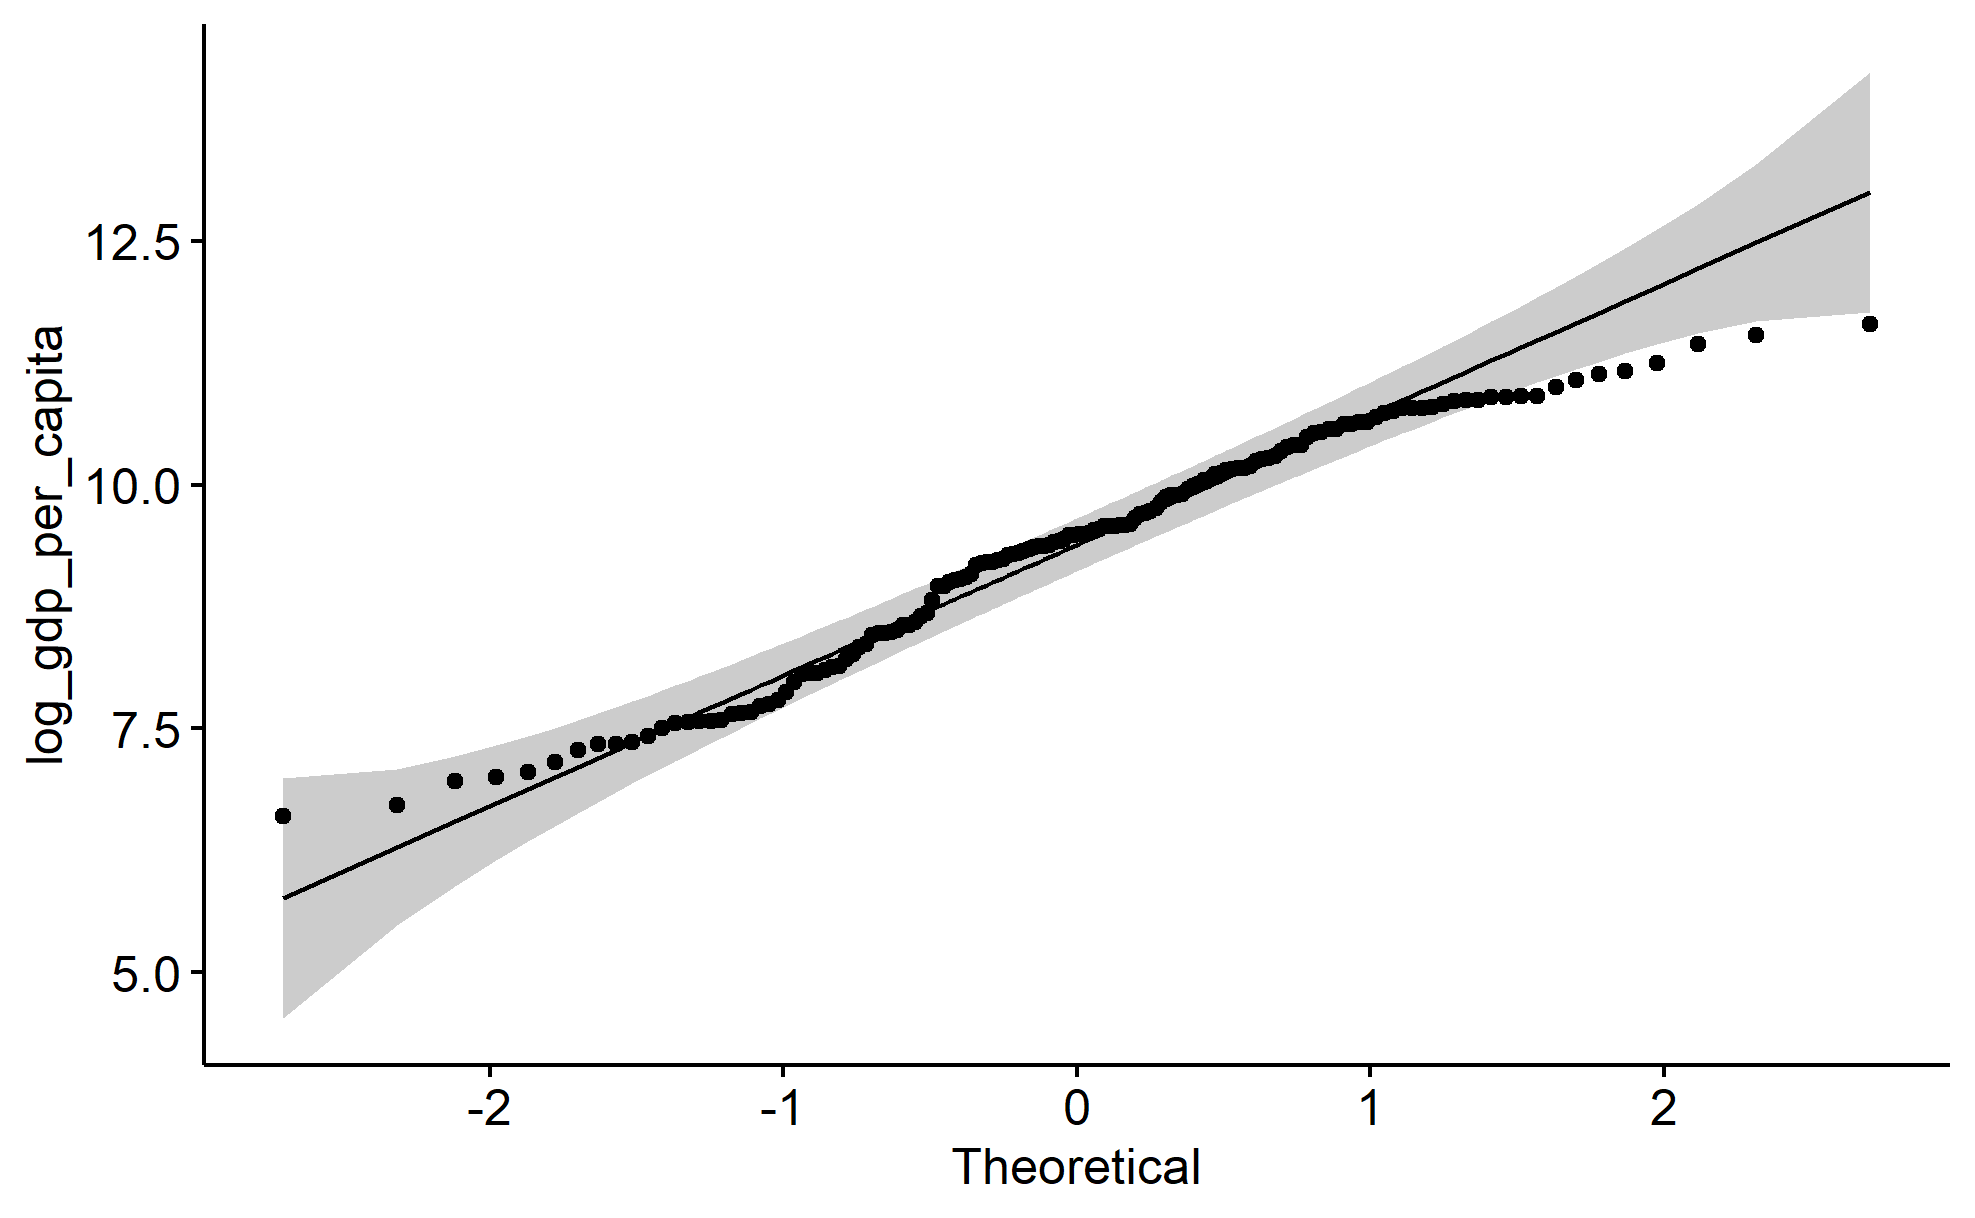
\includegraphics[width=0.5\textwidth]{figures/plot_Ac.png}
    \caption{Normalidad log\_gdp\_per\_capita}
    \label{fig:correlaciones3}
\end{figure}

\newpage
    \item \textbf{Método Delta} \\
    En el punto anterior, se detalló como obtener el coeficiente de correlación Pearson, ahora bien, bajo el contexto del curso resulta fácil ver que esta medida puede tomarse como un estadístico, ya que este contiene todos los datos de las variables $X$ y $Y$.

    A su vez, dado que el procedimiento anterior se realizará con varias variables, podemos decir que obtendremos una serie de estadísticos, esto será de vital importancia para poder utilizar el Método Delta.

    Ahora bien, supongamos que se tiene un estimador $T_n$ para el parámetro $\theta$. Pero, nos interesa la cantidad $g(\theta)$ para alguna función $g$. Resulta natural pensar que $g(T_n)$ es un estimador natural. 

    Justamente de esto trata el Método Delta, el cual se enuncia a continuación:

    \begin{mybox}{Teorema: Método Delta}
        Sea $T_n$ una sucesión de estadísticos tales que:
        
        \begin{equation*}
            \sqrt{n}(T_n - \theta) \xrightarrow[]{d} N(0, \sigma^2(\theta))
        \end{equation*}
        
        Sea $g: \mathbb{R} \longrightarrow \mathbb{R} \text{ diferenciable en } \theta \text{ con } g'(\theta) \neq 0$. 
        Entonces: 

        \begin{equation*}
            \sqrt{n}[g(T_n) - g(\theta)] \xrightarrow[]{d} N(0, [g'(\theta)^2]\sigma^2(\theta))
        \end{equation*}

        \flushright\cite{asymptotic_stats}
    \end{mybox}

    Una vez mencionado el teorema, lo que se busca con él es aproximar la distribución de nuestra variable, por medio de los estadísticos obtenidos al realizar la correlación. 
    \footnote{De momento se agrega únicamente el teorema del Método Delta ya que no se sabe con exactitud cuáles otros sean necesarios.}

\newpage
\begin{lstlisting}[caption={Estimación de la distribución utilizando el método delta}, label=lst:rchunk2 ] 
# Obtenemos la variable de estudio
X <- Data_relevante$life_ladder

# Se calcula el promedio y la varianza de la variable de estudio
prom_X <- mean(X)
var_X <- var(X)

# Se define una funcion dependiente de la variable de estudio Y = 2X + 3
Y <- function(x) 2*x + 3

# Se calcula la derivada de Y con la media de X
Y_prima <- function(x) 2

# Se aplica el metodo delta para estimar la varianza de Y
var_Y <- (Y_prima(prom_X))^2 * var_X

# Se asume que Y sigue una distribucion normal, se determina su promedio y desviacion estandar
mean_Y <- Y(prom_X)
sd_Y <- sqrt(var_Y)
\end{lstlisting}

\end{enumerate}

\textbf{Nota:} Este es el primer acercamiento que se tiene con el modelo delta, se espera perfeccionarlo para las siguientes entregas, esto con ayuda del profesor y las fuentes dadas por el mismo.

\newpage
\subsection{Construcción de fichas de resultados}

\begin{table}[H]
    \caption{Ficha de Resultados 1}
    \begin{center}
        \begin{tabular}{  m{3cm} | m{12cm}  }
        \hline\textbf{ Encabezado} & \textbf{Contenido }\\ \hline
        Nombre de su hallazgo/resultado: &  Correlación Positiva de las variables de interés.\\ \hline
        Resumen en una oración: &  Se pudo encontrar una relación positiva de las variables que queríamos utilizar como factores con el índice de felicidad. 
\\ \hline
        Principal característica: &  Ahora que sabemos que existe esta correlación dado el análisis que realizamos, entonces podemos reforzar esta idea usando más material bibliográfico.\\ \hline
        Problemas o posibles desafíos: &  Cabe la posibilidad de utilizar un método incorrecto para encontrar la correlación o que pase que correlación no implica causalidad, entonces hay que tener especial cuidado con como interpretamos los datos y si la correlación en realidad tiene sentido o no. \\ \hline
        Resumen en un párrafo: & Se utilizó una matriz de correlación para verificar qué variables presentaban una correlación, aunque este análisis se hizo para todas las variables, las que son de nuestro interés, son sólo las 5 mencionadas anteriormente. Se realizó una limpieza de la base de datos para tener unos datos depurados y que no vayan a ensuciar el análisis, también hubieron países que no aportaron ciertos datos, esto pudo haber afectado al análisis de éstos. \\ \hline
        \end{tabular}
    \end{center}
\end{table}

\begin{table}[H]
    \caption{Ficha de Resultados 2}
    \begin{center}
        \begin{tabular}{  m{3cm} | m{12cm}  }
        \hline\textbf{ Encabezado} & \textbf{Contenido }\\ \hline
        Nombre de su hallazgo/resultado: &  Correlación entre corrupción y polución del aire\\ \hline
        Resumen en una oración: &  A partir del análisis de datos, se observó una relación positiva  entre la polución del aire y el índice de corrupción en la base de datos.
\\ \hline
        Principal característica: &  No se esperaba encontrar una correlación positiva entre la corrupción y ninguna variable del modelo, pues se interpreta la corrupción como un concepto de perjuicio en la sociedad. Sin embargo, a partir del análisis pudimos determinar que hay una correlación positiva.\\ \hline
        Problemas o posibles desafíos: &  Hay algo importante que mencionar, y es que correlación no implica causalidad, así que habría que buscar material que apoye específicamente este resultado, para determinar si el análisis de esta variable es o no de importancia. \\ \hline
        Resumen en un párrafo: & Para encontrar este hallazgo se utilizó la matriz de correlación, una hipótesis de este resultado es que al haber corrupción en los gobiernos, las personas encargadas de llevar a cabo la utilización de fondos, podrían no estar utilizando los fondos para lo que deberían ser utilizados, como protección ambiental, por ejemplo. Se podría proponer buscar más información de esta correlación, para determinar si hay o no una relación real, en la tercera bitácora. \\ \hline
        \end{tabular}
    \end{center}
\end{table}

\begin{table}[H]
    \caption{Ficha de Resultados 3}
    \begin{center}
        \begin{tabular}{  m{3cm} | m{12cm}  }
        \hline\textbf{ Encabezado} & \textbf{Contenido }\\ \hline
        Nombre de su hallazgo/resultado: &  Correlación entre Producto Interno Bruto per Capita y el Índice de Percepción de la Corrupción\\ \hline
        Resumen en una oración: &  A partir del análisis de datos, se observó una relación positiva  entre el Producto Interno Bruto y el Índice de Corrupción en la base de datos.
\\ \hline
        Principal característica: &  A partir del análisis de datos se encontró la existencia de una relación positiva entre las dos variables, lo que muestra que a medida que un país tienen un mayor producto interno bruto per capita también presenta un alto índice de percepción de la corrupción.\\ \hline
        Problemas o posibles desafíos: &  Hay algo importante que mencionar, y es que correlación no implica causalidad, así que resulta sensato investigar fuentes fiables que expliquen si existe una relación teórica entre un alto grado de corrupción en relación a un producto interno bruto per capita mayor. \\ \hline
        Resumen en un párrafo: & Para encontrar este hallazgo se utilizó la matriz de correlación, una hipótesis de este resultado podría basarse en el hecho de que un país con un mayor producto interno bruto per capita resulta mas tentador para los gobiernos a dedicarse a actividades éticamente cuestionables con respecto al manejo de finanzas publicas. \\ \hline
        \end{tabular}
    \end{center}
\end{table}

\begin{table}[H]
    \caption{Ficha de Resultados 4}
    \begin{center}
        \begin{tabular}{  m{3cm} | m{12cm}  }
        \hline\textbf{ Encabezado} & \textbf{Contenido }\\ \hline
        Nombre de su hallazgo/resultado: &  Correlación entre clase social y esperanza de vida\\ \hline
        Resumen en una oración: &  A partir del análisis de datos, se observó una relación positiva  entre una alta clase social y la esperanza de vida en la base de datos.
\\ \hline
        Principal característica: &  A partir del análisis de datos se encontró la existencia de una relación positiva entre las dos variables, lo que muestra que a medida que un país presenta una clase social dominante de un estrato más alto tiene a su vez una mayor esperanza de vida.\\ \hline
        Problemas o posibles desafíos: &  Al tratarse la clase social de una variable categórica, las separaciones que existen entre distintos países con la forma en la estructuran su clase dominante no es estandarizada, por lo que pueden existir sesgos. \\ \hline
        Resumen en un párrafo: & Para encontrar este hallazgo se utilizó la matriz de correlación, una clase social dominante de un estrato más alto, va a tener un acceso mas facilitado a servicios de una mayor calidad, incluyendo los de salud, lo cual esta demostrado mediante estudios anteriores que influye de forma positiva en la esperanza de vida. \\ \hline
        \end{tabular}
    \end{center}
\end{table}

\begin{table}[H]
    \caption{Ficha de Resultados 5}
    \begin{center}
        \begin{tabular}{  m{3cm} | m{12cm}  }
        \hline\textbf{ Encabezado} & \textbf{Contenido }\\ \hline
        Nombre de su hallazgo/resultado: &  Correlación entre Índice de Felicidad y Log del Producto Interno Bruto\\ \hline
        Resumen en una oración: &  A partir del gráfico de dispersión, se observó una relación positiva  entre el Índice de Felicidad y el Log del Producto Interno Bruto. \\ \hline
        Principal característica: &  A partir del análisis de datos se encontró la existencia de una relación positiva entre las dos variables, lo que se muestra de forma positiva con la literatura que se ha desarrollado, que denota una relación positiva entre la Felicidad y variables económicas, siendo el Producto Interno Bruto la más importante de estas.\\ \hline
        Problemas o posibles desafíos: &  La Felicidad se observa como una variable compleja para la cual no resulta completamente adecuado realizar un análisis enfocado únicamente en el área económica, sino que presente elementos psicológicos y sociológicos \\ \hline
        Resumen en un párrafo: & Para encontrar este hallazgo se utilizó tanto la matriz de correlación como el gráfico de dispersión, valores de magnitudes cada vez mayores están relacionados con un mayor Índice de Felicidad según la literatura que se abarca en el estudio presente. \\ \hline
        \end{tabular}
    \end{center}
\end{table}

% --- Bitácora 3 ---
\chapter{Bitácora 3} \label{bitacora3}

Las sugerencias y correcciones de la Bitácora 2 se detallan en los Apéndices [\ref{Apendices}], mientras que los cambios fueron realizados propiamente en la Bitácora 2 [\ref{bitacora2}]. 

\section{Parte de planificación}

\subsection{Análisis de modelación}

Se mejoró significativamente el código utilizado en la investigación para lograr que fuera completo, robusto y reproducible. A grandes rasgos, el código es capaz de cargar los datos de manera automática, inmediatamente después realiza un análisis descriptivo completo de los datos, luego ajusta e inicializa el modelamiento por su cuenta, esto con las metodologías previstas, por último, realiza un análisis de los resultados de los modelos previos. Todo a su vez debidamente comentado.\\

Al mismo tiempo, nos parece oportuno recordar que el proyecto se encuentra en el repositorio de \textbf{\href{https://github.com/bluke7ide/Proyecto_Estadistica}{GitHub}} [\ref{github}], donde se podrán ver todas las versiones y a su vez los resultados finales.
\pagebreak

\subsection{Construcción de fichas de resultados}

\begin{table}[H]
    \caption{Ficha de Resultados 1}
    \begin{center}
        \begin{tabular}{  m{3cm} | m{12cm}  }
        \hline
        \textbf{ Encabezado} & \textbf{Contenido }\\ 
        \hline
        Nombre de su hallazgo/resultado: & Correlación positiva entre el acceso a la electricidad y el Índice de Felicidad.\\ 
        \hline
        Resumen en una oración: & Dados los datos que se utilizaron en el estudio, se encontró que sí hay una evidencia empírica de esta correlación.\\ 
        \hline
        Principal característica: & Este valor obtenido ayuda a reforzar lo que se ha visto en el material teórico de referencia en el estudio.\\ 
        \hline
        Problemas o posibles desafíos: &  Cabe la posibilidad de que los datos que estamos utilizando estén sesgados o que el método de correlación de Pearson no sea el más óptimo para esta relación. \\ \hline
        Resumen en un párrafo: & Se utilizó la fórmula del índice de correlación de Pearson para encontrar una distancia estadística entre dos variables, funciona de manera similar a una matriz de correlación, pero difieren en que la correlación de Pearson es una relación lineal entre las variables que nos permite analizar los datos con un enfoque diferente. \\ 
        \hline
        \end{tabular}
    \end{center}
\end{table}

\begin{table}[H]
    \caption{Ficha de Resultados 2}
    \begin{center}
        \begin{tabular}{  m{3cm} | m{12cm}  }
        \hline
        \textbf{ Encabezado} & \textbf{Contenido }\\ 
        \hline
        Nombre de su hallazgo/resultado: & Correlación positiva entre la clase social y el Índice de Felicidad.\\ 
        \hline
        Resumen en una oración: & Se encontró una tendencia a que aquellos en las clases de ingresos más altas tiendan a reportar niveles más altos de felicidad.\\ 
        \hline
        Principal característica: &  Dado que esta variable es discreta, y está compuesta por 4 clases propiamente, se puede observar de una manera muy fuerte que efectivamente la felicidad reportada por las personas aumenta conforme suben de clase social. \\ 
        \hline
        Problemas o posibles desafíos: &  Aunque el gráfico sugiere una asociación entre ingresos y felicidad, otros factores no considerados en el análisis podrían influir en la percepción de la felicidad. Además, la presencia de valores atípicos podría distorsionar la interpretación de la relación entre las variables. \\ 
        \hline
        Resumen en un párrafo: & El análisis revela una relación ascendente entre la clase social y la felicidad percibida, indicando que aquellos en clases sociales más altas tienden a reportar niveles más altos de felicidad. Este hallazgo sugiere que el aumento en los ingresos está asociado con una mayor percepción de bienestar, resaltando la importancia del estatus socioeconómico en la calidad de vida de los individuos. Sin embargo, es importante considerar que este análisis no tiene en cuenta otros factores que pueden influir en la percepción de la felicidad, esto puede corroborarse con los valores atípicos encontrados en la misma. \\ 
        \hline
        \end{tabular}
    \end{center}
\end{table}

\begin{table}[H]
    \caption{Ficha de Resultados 3}
    \begin{center}
        \begin{tabular}{  m{3cm} | m{12cm}  }
        \hline
        \textbf{ Encabezado} & \textbf{Contenido }\\ 
        \hline
        Nombre de su hallazgo/resultado: & Correlación positiva entre el acceso al agua y el Índice de Felicidad.\\ 
        \hline
        Resumen en una oración: & Se encontró una relación positiva entre los índices de acceso al agua y el de felicidad, de un $0.71$. \\
        \hline
        Principal característica: &  Esta es una de las variables que presenta más relación lineal con el índice de felicidad, de donde podemos inferir que el acceso al agua es uno de los determinantes importantes del índice de felicidad.\\ 
        \hline
        Problemas o posibles desafíos: &  Los datos podrían verse manipulados a conveniencia o que la relación entre los índices no sea lineal. \\ 
        \hline
        Resumen en un párrafo: & Se utilizó el método de correlación de pearson, que busca la relación lineal entre dos variables, de donde el valor de 1 índica una relación lineal positiva absoluta, en este caso, encontramos que el índice de correlación fue del $0.71$ lo cual es un número bastante representativo de la relación que existe entre estas variables. \\ 
        \hline
        \end{tabular}
    \end{center}
\end{table}

\begin{table}[H]
    \caption{Ficha de Resultados 4}
    \begin{center}
        \begin{tabular}{  m{3cm} | m{12cm}  }
        \hline
        \textbf{ Encabezado} & \textbf{Contenido }\\ 
        \hline
        Nombre de su hallazgo/resultado: & Correlación positiva entre el Producto Interno Bruto y el Índice de Felicidad.\\ 
        \hline
        Resumen en una oración: & Se encontró una relación positiva entre el índice del log Producto Interno Bruto y el índice de felicidad, de un $0.81$, siendo este nuestro índice más importante.  \\ 
        \hline
        Principal característica: &  Esta variable representa nuestro índice de correlación más importante dado el método de correlación de Pearson. Se esperaba desde el anteproyecto que esta relación fuera la más importante dadas las referencias bibliográficas que se utlizaron para la investigación y con los datos que se utilizaron logramos obtener un refuerzo empírico de esta relación.\\ 
        \hline
        Problemas o posibles desafíos: & La cultura de los países donde conseguimos los datos puede afectar a este resultado, es decir, países con economías capitalistas tienden a asociar el ingreso con una mayor felicidad, por lo cual los datos podrían no ser representativos a economías donde no se sigue esta ideología. \\ \hline
        Resumen en un párrafo: & Se utilizó el método de correlación de pearson, que busca la relación lineal entre dos variables, de donde el valor de 1 índica una relación lineal positiva absoluta, en este caso, encontramos que el índice de correlación fue del $0.71$ lo cual es un número bastante representativo de la relación que existe entre estas variables. \\ 
        \hline
        \end{tabular}
    \end{center}
\end{table}

\begin{table}[H]
    \caption{Ficha de Resultados 5}
    \begin{center}
        \begin{tabular}{  m{3cm} | m{12cm}  }
        \hline
        \textbf{ Encabezado} & \textbf{Contenido } \\ 
        \hline
        Nombre de su hallazgo/resultado: & Aproximación empírica de la densidad del Índice de Felicidad con una Normal.\\ 
        \hline
        Resumen en una oración: & Se graficó de manera continua el histograma del Índice de Felicidad y se comparó con una distribución Normal de parámetros media muestral y varianza muestral.\\ 
        \hline
        Principal característica: & Para realizar esta comparación, se utilizó una normal de parámetros media muestral y varianza muestral, ya que estos son los estimadores de máxima verosimilitud del parámetro y por ende es nuestra mejor aproximación que tenemos de éste. Para esto se utlizaron funciones de R con el fin de poder graficar el histograma continuamente y hacer la comparación más evidente.\\ 
        \hline
        Problemas o posibles desafíos: & Que el método de estimación que utilizamos para la distribución normal no estén cerca o que la cantidad de datos que usamos para sacar el estimador de máxima verosimilutd no fueron suficientes para poder aproximar la distribución.\\ 
        \hline
        Resumen en un párrafo: & Se comparó una versión continua del histograma para poder evidenciar qué tanto del área de una normal, con parámetros media muestral y varianza muestral, es llenado por esta versión continua del histograma.\\ 
        \hline
        \end{tabular}
    \end{center}
\end{table}

\begin{table}[H]
    \caption{Ficha de Resultados 6}
    \begin{center}
        \begin{tabular}{  m{3cm} | m{12cm}  }
        \hline
        \textbf{ Encabezado} & \textbf{Contenido }\\ 
        \hline
        Nombre de su hallazgo/resultado: & Evaluación del comportamiento del Índice de Felicidad como una distribución normal.\\ 
        \hline
        Resumen en una oración: & El gráfico de cuantiles del Índice de Felicidad muestra que los datos se alinean bien con la línea diagonal en el medio, con pequeñas desviaciones a partir de los extremos.\\ 
        \hline
        Principal característica: & Dado que la mayoría de los datos del Índice de Felicidad se alinean con la línea diagonal, se puede observar entonces que los datos siguen una distribución aproximadamente normal en el rango central. \\ 
        \hline
        Problemas o posibles desafíos: & Las pequeñas desviaciones en los extremos sugieren que podría haber ligeras diferencias de normalidad en las colas de la distribución, pero no parecen ser tan significativas.\\ 
        \hline
        Resumen en un párrafo: &  El gráfico de cuantiles del Índice de Felicidad revela que los datos se alinean bien con la línea diagonal que representa la distribución normal teórica, especialmente en el rango central. A partir de los valores de $-1,5$ y $1,5$, se observa una ligera desviación de los puntos de la línea diagonal, indicando que hay pequeñas diferencias de normalidad en los extremos de la distribución. En general, estos resultados sugieren que el Índice de Felicidad sigue una distribución aproximadamente normal, lo que es favorable para la aplicación de métodos estadísticos que asumen normalidad. \\ 
        \hline
        \end{tabular}
    \end{center}
\end{table}

\begin{table}[H]
    \caption{Ficha de Resultados 7}
    \begin{center}
        \begin{tabular}{  m{3cm} | m{12cm}  }
        \hline
        \textbf{ Encabezado} & \textbf{Contenido }\\ 
        \hline
        Nombre de su hallazgo/resultado: & Evaluación del comportamiento del log PIB per cápita como una distribución normal.\\ 
        \hline
        Resumen en una oración: & En el gráfico de cuantiles de log PIB per cápita, los datos se alinean mayormente con la línea diagonal, indicando una posible distribución normal. \\ 
        \hline
        Principal característica: & La mayoría de los puntos de la variable log PIB per cápita coinciden con la línea diagonal, lo que sugiere una posible distribución normal en la región central del gráfico.\\ 
        \hline
        Problemas o posibles desafíos: & Se detectan pequeñas divergencias en los extremos del gráfico, lo que podría implicar diferencias en la normalidad en las colas de la distribución.\\ 
        \hline
        Resumen en un párrafo: & El gráfico de cuantiles de log PIB per cápita muestra una adecuada alineación de los datos con la línea diagonal, especialmente en el área central del gráfico, lo que sugiere una posible distribución normal en esa sección. No obstante, se observan algunas divergencias en los extremos, indicando posibles variaciones en la normalidad en esas áreas. A pesar de estas variaciones, los resultados sugieren que la variable log PIB per cápita podría aproximarse a una distribución normal, lo que nuevamente facilitaría la aplicación de métodos estadísticos que asumen normalidad. \\ 
        \hline
        \end{tabular}
    \end{center}
\end{table}

\begin{table}[H]
    \caption{Ficha de Resultados 8}
    \begin{center}
        \begin{tabular}{  m{3cm} | m{12cm}  }
        \hline
        \textbf{ Encabezado} & \textbf{Contenido }\\ 
        \hline
        Nombre de su hallazgo/resultado: & Normalización del Índice de Felicidad por medio del Teorema del Límite Central. \\ 
        \hline
        Resumen en una oración: & Se consiguió normalizar la variable del Índice de Felicidad mediante el uso del Teorema del Límite Central.\\ 
        \hline
        Principal característica: & Para lograr llegar a cabo la normalización del Índice de Felicidad, se utilizaron los estadísticos de máxima verosimilitud y el Teorema del Límite Central.\\ 
        \hline
        Problemas o posibles desafíos: &  El Teorema del Límite Central implícitamente requiere de una cantidad muy grande de datos, mientras que la cantidad de datos nuestra está limitada a menos poco menos de 200.\\ 
        \hline
        Resumen en un párrafo: & Haciendo uso de los estadísticos de máxima verosimilitud y el Teorema del Límite Central, se ha conseguido normalizar la variable indicadora de la Felicidad, esto toma más valor al juntarlo con el resultado previamente conseguido, donde vimos que el Índice de Felicidad tiende a ser normal. Sin embargo, existe una limitante al hacer uso de este teorema, y es que la cantidad de datos es limitada, por lo que sería importante considerar este factor.\\ 
        \hline
        \end{tabular}
    \end{center}
\end{table}
\newpage

\subsection{Ordenamiento de los elementos de reporte}

En primer lugar, se procede a identificar los elementos primarios y secundarios del trabajo.

\begin{table}[H]
    \caption{Identificación de los elementos primarios y secundarios}
    \begin{center}
        \begin{tabular}{  m{7cm}  m{7cm}  }
        \hline
        \multicolumn{2}{c}{\textbf{Elementos de reporte}} \\
        \hline
        \textbf{Primarios} & \textbf{Secundarios} \\
        \hline
        Método Delta Multivariable & Identificación de las variables relevantes.\\ 
        Coeficiente de Correlación de Pearson & Elección de teoría bibliográfica\\ 
        Pruebas de Shapiro-Wilk & Matriz de correlaciones\\
        Transformación Z de Fisher & Intervalos de confianza sobre los índices de correlaciones\\
        Interconexión entre indicadores socioeconómicos & Teorema del Límite Central para normalizar los datos.\\ 
        Índices de correlaciones positivos & Contradicciones encontradas en la bibliografía.\\
        Comportamientos de variables como variables normales & Limitaciones y complejidades del concepto de felicidad.\\
        \hline
        \end{tabular}
    \end{center}
\end{table}

\pagebreak

A continuación se procede a realizar una guía de todo lo realizado hasta el momento:

\begin{table}[H]
    \caption{Tabla guía de escritura}
    \begin{center}
        \begin{tabular}{  m{2cm}  m{8cm}  }
        \hline
        Sección & Tema a tratar \\
        \hline
        Introducción & 1. Definición de Indicadores Socioeconómicos. (Primario) \\
        & 2. Definición de Felicidad como concepto y como variable de estudio. (Primario) \\
        & 3. Identificación de las variables relevantes. (Secundario)\\ 
        & 4. Selección de los modelos. (Primario)\\ 
        & 5. Recolección de teoría bibliográfica. (Secundario)\\ 
        & 6. \\
        \hline
        Metodología & 1. Limpieza de datos. (Primario) \\
        & 2. Matriz de correlaciones. (Secundario). \\
        & 3. Coeficiente de correlación de Pearson. (Primario) \\
        & 4. Método Delta Multivariable. (Primario) \\
        & 5. Pruebas de Shapiro-Wilks. (Primario) \\
        & 6. Transformación Z de Fisher. (Primario) \\
        & 7. Teorema del Límite Central para normalizar los datos. (Secundario)\\
        \hline
        Resultados & 1. Índices de correlaciones positivos. (Primario)\\
        & 2. Comportamientos de variables como variables normales. (Primario)\\
        & 3. Intervalos de confianza sobre los índices de correlaciones.(Secundario)\\ 
        & 4. Contradicciones encontradas en la bibliografía. (Secundario)\\
        & 5. Limitaciones y complejidades del concepto de felicidad. (Secundario)\\
        \hline
        \end{tabular}
    \end{center}
\end{table}

\newpage

\section{Parte de escritura}

En esta sección se va realizar un contraste de la historia que se describe en la bibliografía utilizada, es decir, por un lado se tiene la historia descrita por la investigación teórica, mientras que por el otro se tiene una historia creada por los datos que encontramos en la investigación. Esto con el fin de reforzar o refutar la teoría que encontramos como marco teórico, la cual motivó la investigación.\\

Inicialmente, la investigación comenzó con la idea de examinar la relación que existe entre el progreso socioeconómico de un país con el Índice de Felicidad, de donde se consideró inicialmente ver específicamente las variables de acceso a la electricidad, acceso al agua, PIB per cápita, entre otros. (Esto porque aún no estaba delimitado del todo las variables que se iban a utilizar en el estudio). La motivación inicial fue ver el impacto qué tienen ciertas variables socioeconómicas sobre nuestra variable de interés (Índice de Felicidad). De igual manera, como mencionamos en partes anteriores, esta investigación podría tener utilidad en el ámbito político, donde se podrían tomar decisiones para optimizar este Índice y de paso tener un progreso socioeconómico.\\

Según el análisis bibliográfico realizado en etapas anteriores de la bitácora, todas las referencias apuntaban a que la relación entre variables socioeconómicas y el Índice de Felicidad tendrían una correlación positiva. Pero antes de adentrarnos con esa conclusión, es importante mencionar que esta investigación sin un valor socioeconómico no tendría sentido, por lo que es importante definir este, de donde según el Instituto Nacional del Cáncer (2024) este valor socioeconómico se define como una ``descripción de la situación de una persona según la educación, los ingresos y el tipo de trabajo que tiene.'' Cabe recalcar que este mismo estudio (del Instituto Nacional del Cáncer, 2024.) se hace mención de que ``las personas con un nivel socioeconómico bajo, a menudo, tienen menos acceso a recursos financieros, educativos, sociales y de salud que aquellas que tienen un nivel socioeconómico más alto.'' Como podemos observar ya se encontraban evidencias de esta relación. \\

También se trató de definir el concepto de felicidad, esto para tener un orden conceptual y saber a qué nos estamos refiriendo cada vez que hablamos de este concepto, sin embargo, definir qué es el concepto de felicidad era un trabajo arduo y no encontramos una definición que se adaptara a esta investigación, más que todo porque este concepto puede ser algo subjetivo de persona a persona, por lo que habría que pensar un agregado y definir la felicidad o al menos un índice según ciertos aspectos en común que hace que una persona valide sus derechos y sus necesidades. Según Roberto Gutiérrez (2023), los Índices de Felicidad que publica la ONU se determinan mediante el PIB per cápita, el apoyo social, la esperanza de vida saludable, la libertad de tomar decisiones vitales, la generosidad y la percepción de la corrupción. Sin embargo, vea que apesar de que la ONU define estos índices, aún deja muchos aspectos sociales de la ``felicidad'' por fuera. \\

Ahora bien, en un intento por crear una correlación positiva entre las variables socioeconómicas con el Índice de Felicidad, notamos que a pesar de que hay evidencia empírica de que los datos parecen tener una relación positiva, hay contraejemplos, lo que no nos deja hacer una generalización, esto lo mencionaban los autores Aguilar, Pámies, Foucault, que mencionaban que ``no se puede generalizar que las políticas encaminadas a maximizar la felicidad nacional aumentarán los datos económicos''. Esto hace referencia a que hay un trade-off entre aumentar la felicidad, o mejorar el crecimiento económico de un país, lo cual es un claro contraejemplo de lo que estamos queriendo analizar. Sin embargo, la evidencia encontrada en la literatura sugiere que tener factores socioeconómicos puede implicar tener un mayor grado de felicidad, y que lo recíproco es falso en general. \\

Debido a esta relación, se intenta utilizar la felicidad para comparar el progreso socioeconómico de los países y así lograr una amplia gamma de enfoques, como por ejemplo factores sociales, dado que ``el hecho de tener un buen estado de salud incrementa la probabilidad de sentirse feliz entre $18.1$ y $28.9$ puntos porcentuales respecto a los que no manifiestan dicho estado.''\\

Por ello, en etapas temprana de esta investigación se pensó en utilizar una base de datos que contuviera la información acerca de varios países, para lograr tener un resultado más conciso. Además de buscar la correlación existente entre las variables y analizar cómo se comporta la distribución del Índice de Felicidad. Desde un principio de la investigación se supo que se tenía que utilizar la metodología del coeficiente de correlación lineal de Pearson, para ver la relación positiva-negativa de las variables y luego aplicar el método delta para obtener los resultados deseados. Estos métodos se describen a continuación: \\

\begin{enumerate}
    \item \textbf{Coeficiente de Correlación Lineal de Pearson} \\
    
    El coeficiente de correlación de Pearson es un índice que mide el grado de covariación entre distintas variables relacionadas linealmente. Supongamos que se tienen dos variables $X$, $Y$. Se define el coeficiente de correlación de Pearson entre estas dos variables como $r_{xy}$ donde:
    
    \begin{equation*}
        -1 \leq r_{xy} \leq 1
    \end{equation*} 
    
    Es importante mencionar que la magnitud de la relación vienen especificada por el valor numérico del coeficiente, mientras que el signo refleja la dirección de tal valor. Esto quiere decir que una relación de $+1$ es igual de fuerte a una relación $-1$, solamente cambia el sentido de esta.\\

    Una correlación positiva entre dos variables indica que a medida que una de ellas aumenta, la otra también lo hace. En el caso de que ambas aumenten en igual medida, se dice que son perfectamente positivas. De manera similar, una correlación negativa entre dos variables indica que a medida que una de ellas aumenta, la otra disminuye. En el caso de que ambas cambien en igual magnitud, se dice que son perfectamente negativas.\\

    El coeficiente de Pearson viene dado por la siguiente fórmula:
    
    \begin{equation}
         r_{xy} = \frac{\sum Z_x Z_y}{N} 
    \end{equation}
   
    Donde: 
    
    \begin{itemize}
        \item $Z_x$ es la desviación estándar de X
        \item $Z_y$ es la desviación estándar de Y
        \item N es la cantidad de datos 
    \end{itemize}

    \item \textbf{Método Delta} \\
    
    En el punto anterior, se detalló como obtener el coeficiente de correlación Pearson, note que esta medida puede verse como un estadístico, ya que contiene todos los datos de las variables $X$ y $Y$. A su vez, dado que el procedimiento anterior se realizará con varias variables, podemos decir que obtendremos una serie de estadísticos, esto será de vital importancia para el Método Delta. \\

    \begin{theorem}[Método Delta] 
    Sea $T_n$ una sucesión de estadísticos tales que:
        \begin{equation*}
            \sqrt{n}(T_n - \theta) \xrightarrow[]{d} N(0, \sigma^2(\theta))
        \end{equation*}

    Sea $g: \mathbb{R} \longrightarrow \mathbb{R}$ diferenciable en $\theta$ con $g'(\theta) \neq 0$. Entonces:

        \begin{equation}
            \sqrt{n}[g(T_n) - g(\theta)] \xrightarrow[]{d} N(0, [g'(\theta)^2]\sigma^2(\theta))
        \end{equation}
    \end{theorem}

    Dicho el teorema, lo que se busca entonces es aproximar la distribución de nuestra variable, por medio de los estadísticos obtenidos al realizar la correlación. 
\end{enumerate}

Para este punto de la investigación, teníamos pensado sólo aplicar las técnicas descritas anteriormente junto al análisis de datos correspondiente, pero después de avanzar en dicho estudio, descubrimos que podíamos aplicar otras metodologías, las cuales vamos a comentar más adelante, cuando demos una explicación detallada de cuál fue la historia que nosotros obtuvimos al hacer esta investigación. A grandes rasgos, se expandió el uso de coeficiente de correlación a más de un método, siendo estos el de Kendall y el de Spearman, esto para poder realizar comparaciones de los mismos y obtener coeficientes más certeros. Al mismo tiempo, se implementó el uso de pruebas de Shapiro-Wilk, esto para evaluar si la muestra utilizada seguía una distribución normal, con el fin de utilizarlo como previa para más adelante aplicar el Método Delta Multivariado. Por último, se calcularon los intervalos de confianza haciendo uso nuevamente del coeficiente de correlación de Pearson, utilizando el Método de la Transformación Z de Fisher, mismo que se deriva del Método Delta Multivariable.\\

\textbf{\textit{Nuestra Historia:}} \\

Como parte inicial, se realizó una limpieza de la base de datos para tener los datos depurados y que no vayan a ensuciar el análisis que se realizaría posteriormente, también hubieron países que no aportaron ciertos datos, esto pudo haber afectado al análisis de éstos ya que no teníamos una completitud de estos, además de tener una cantidad de datos menos con la cual trabajar.\\

Una vez se tuvieron los datos limpios, para nuestra investigación se utilizó una matriz de correlación, esto con el fin de verificar qué variables presentaban una correlación tanto positiva como negativa con nuestra variable de interés asociada, la cuál es el Índice de Felicidad. Aunque este análisis se hizo para todas las variables, las que son de nuestro interés, son sólo las 4 mencionadas anteriormente (acceso a la electricidad, agua, PIB per cápita, e Índice de corrupción) ya que fueron las que obtuvieron una relación con mayor magnitud. \\

Como hemos venido desarrollando esta sección, desde el comienzo de esta investigación creíamos, dado la evidencia bibliográfica, que nosotros también íbamos a encontrar relaciones positivas entre nuestras variables, para ello, cuando utilizamos el método de coeficiente de relación de Pearson encontramos que existe una relación positiva del acceso a la electricidad y el Índice de Felicidad, en un 0.74. Esto lo que significa, según cómo anteriormente habíamos explicado el método de correlación, es que hay una correlación positiva lineal entre estas variables. Esta correlación fue hecha usando las librerías que proporciona R para este trabajo, pero el método de cálculo de manera manual, es mediante la fórmula que estamos agregando a continuación: \\

\textbf{Coeficiente de Correlación de Pearson} \\

\begin{equation}
         r_{xy} = \frac{\sum Z_x Z_y}{N} 
    \end{equation}
   
    Donde: 
    
    \begin{itemize}
        \item $Z_x$ es la desviación estándar de X
        \item $Z_y$ es la desviación estándar de Y
        \item N es la cantidad de datos 
    \end{itemize}

Gracias a esta fórmula, pudimos encontrar una relación positiva también entre la variable de acceso al agua, el cual es un factor indispensable en la vida humana. A su vez, podemos afirmar gracias al estudio bibliográfico y al estudio realizado, que sí existe una correlación tanto del acceso a la luz como del acceso al agua con el índice de felicidad, ya que el coeficiente de Pearson nos dio $0.71$ para el caso del agua, el cual es un valor bastante cercano a 1, el cual significa relación casi perfecta. Además, esto se vio reforzado en el resultado de matriz de correlaciones, la cual nos dio una correlación fuerte entre estas variables. \\

Por otro lado, otra variable que ha sido método de estudio en otras investigaciones es el Índice de Percepción de la Corrupción contra el Índice de Felicidad, donde encontramos que también presentan una correlación bastante significativa del 0.8, lo cual indica que este es uno de las variables más importantes en este estudio. Es importante recalcar al lector, que esta correlación dio positiva, es decir, entre mayor Índice de Percepción de Corrupción tengamos, mayor Índice de Felicidad deberíamos tener. Ahora, la interpretación que recibe el Índice de Percepción de la Corrupción se interpreta como ``Entre más cercano de 0, se percibe que hay más corrupción y entre más cercano al 1, entonces se percibe que hay menos corrupción''. Entonces si este índice se interpretara de manera diferente, es de esperar que la correlación del coeficiente de Pearson nos diera un número cercano a $-1$. Este es un resultado que se ha visto en las bibliografías utilizadas, pues las personas tienen una aversión a la corrupción de las entidades gubernamentales que afecta de manera directa a su felicidad. \\

Por último, y no menos importante, la correlación más fuerte dado este método que realizamos se da entre las variables Índice de Felicidad y el logaritmo del Producto Interno Bruto, el cual nos dio un índice de $0.81$. Como vimos en la etapa de análisis bibliográfico, esta variable es la que más se asocia a los Índices de Felicidad, aunque puede no parecer una sorpresa, pues es de esperar que en una economía capitalista, más dinero implique mayor grado de satisfacción, que ya sea directa o indirectamente puede traducirse en mayor disfrute y por ende, en mayor felicidad. \\ 

Por otra parte, el considerar el Método Delta como una metodología a utilizar, nos abrió la puerta hacia su versión más fuerte, la del Método Delta Multivariable. En esta fase, este método se utilizó para conseguir la relación entre nuestras variables predictoras y nuestra variable de estudio, es importante mencionar que como variables predictoras se utilizaron las siguientes variables:

\begin{itemize}
    \item Acceso a la Electricidad

    \item Acceso al Agua

    \item Log PIB per cápita

    \item Índice de Percepción de la Corrupción
\end{itemize}

\pagebreak
\textbf{Método Delta Multivariable} \\

Dado que no se ha mencionado aún, nos parece oportuno presentar el Método Delta Multivariable:\\

    \begin{theorem}[Método Delta Multivariable] 
        Sean $f$ y $g$ funciones que reciben como parámetros vectores que retornan valores escalares, la covarianza asintótica entre $f(T)$ y $g(T)$ es aproximadamente:
        
        $$Cov(f(T), g(T)) \approx \frac{1}{n}\sum_{j=1}^p\sum_{k=1}^p\frac{\delta f}{\delta \theta_j}\frac{\delta g}{\delta \theta_k}\sigma_{jk}$$
    
        De igual manera resulta necesario calcular la varianza de la función que recibe como parámetros los estadísticos
    
        $$Var(f(T)) \approx \frac{1}{n}\sum_{j=1}^p(\frac{\delta f}{\delta \theta_j})^2\sigma_{jk}$$
    
        Esto con la finalidad de calcular el coeficiente de correlación de Pearson
    
        $$\rho=\frac{S_{xy}}{\sqrt{S_{xx}S_{yy}}}$$

    \end{theorem} 

Este método nos ayudó a conseguir de manera directa los coeficientes de correlación de Pearson, mismos que se utilizaron para nuestra conclusión de cómo influyen las variables socioeconómicas de interés en nuestra variable Índice de Felicidad. Adjuntamos también la tabla con los coeficientes que arrojó nuestro investigación en la parte del análisis de datos: \\

\begin{table}[H]
    \caption{Coeficiente de correlación de Pearson}
    \centering
    \begin{tabular}{l|*{6}{>{\raggedleft\arraybackslash}p{1.2cm}}}
        \hline
        Predictor & $R^2$ & $R$ & IC Inf & IC Sup \\ \hline
        log\_gdp\_per\_capita & 0,81 & 0,90 & 0,71 & 0,84 \\
        electricity\_access   & 0,67 & 0,75 & 0,56 & 0,74 \\
        water\_access & 0,71 & 0,79 & 0,60 & 0,77 \\
        cpi & 0,72 & 0,80 & 0,61 & 0,78 \\ \hline
    \end{tabular}
\end{table}

Inmediatamente después, utilizamos el método $Z$ de Fisher, el cual sirve para determinar los intervalos de confianza dado un coeficiente de correlación de Pearson, el cual ya se explicó el porqué se utilizó. \\

\pagebreak

\textbf{Transformación $Z$ de Fisher} \\

La transformación $Z$ de Fisher es una fórmula que nos permite transformar el coeficiente de correlación de Pearson $r$ y convertirlo a un valor $z_r$, el cual nos va a permitir calcular un intervalo de confianza para el coeficiente de correlación de Pearson. \\

De igual forma, nos parece oportuno y adecuado presentar formalmente este teorema, ya que su implementación se dio gracias al nuevo rumbo que obtuvo la investigación. \\

    \begin{theorem}[Transformación $z$ de Fisher]
        $$z_r=\frac{1}{2}ln(\frac{1+\rho}{1-\rho})=tan^{-1}(\rho)$$
    
        La $z_r$ es la transformación que estabiliza y normaliza la varianza, esto se puede comprobar aplicando el método delta:
    
        $$\frac{\delta z}{\delta \rho}=\frac{1}{1-\rho^2}$$
    
        Para calcular el intervalo de confianza es necesario encontrar la cota superior e inferior del log:
    
        $$U=z_r + \frac{z_{1-\frac{\alpha}{2}}}{\sqrt{n-3}}$$    
    
        $$L=z_r - \frac{z_{1-\frac{\alpha}{2}}}{\sqrt{n-3}}$$
    
        Una vez obtenidas las cotas, el intervalo de confianza se puede calcular de la siguiente manera:
    
        $$T=[\frac{e^{2L}-1}{e^{2L}+1},\frac{e^{2U}-1}{e^{2U}+1}]$$

    \end{theorem}

Es importante destacar que este intervalo nos otorga un rango en el cual se encuentra el verdadero coeficiente de correlación de Pearson. Recordemos que este intervalo se interpreta como ``Con una probabilidad del 95\%, nuestro parámetro va a estar dentro de este intervalo''.\\

Por otro lado, uno de los objetivos principales de la investigación, era determinar la distribución que tenía la variable aleatoria Índice de Felicidad, por lo cual decidimos utilizar las Pruebas de Shapiro-Wilks en vez de las Pruebas de Kolmogorov-Smirnov, esto porque el método proporcionado por Shapiro-Wilks utiliza en su cálculo las covarianzas de las variables involucradas, razón por la cual resulta más natural escoger esta prueba estadística de normalidad, esto porque hemos estado trabajando con las covarianzas en los cálculos del coeficiente de correlación de Pearson. \\

\pagebreak

\textbf{Prueba Shapiro-Wilks} \\

Nuevamente, procedemos a presentar y explicar cómo funciona este método, ya que conocer la teoría que hay detrás es de vital importancia y sumamente enriquecedor para generar resultados de calidad. Es importante mencionar que que a la hora de calcularlo en la investigación, utilizamos directamente las funciones de R (shapiro.test(X) con X como un vector numérico): \\

A grandes razgos, este método corresponde a una prueba de normalidad, que busca determinar si un conjunto de datos sigue una distribución normal. \\

    \begin{theorem}[Pruebas de Shapiro-Wilks] 
    
        Inicialmente se establecen dos hipótesis:

        \begin{enumerate}
            \item $H_0:$ Los datos siguen una distribución normal
            \item $H_1:$ Los datos no siguen una distribución normal
        \end{enumerate}
    
        Se calcula W, el cual mide la similitud entre los datos y una distribución normal.
    
        $$W = \frac{\left(\sum_{i=1}^n a_i x_{(i)}\right)^2}{\sum_{i=1}^n (x_i - \bar{x})^2}$$
    
        Donde $x_{(i)}$ es el $i$-ésimo valor mas pequeño de la muestra. \\
    
        Los coeficientes $a_i$ se definen por:
    
        $$(a_1, \ldots, a_n) = \frac{m^T V^{-1}}{C}$$
    
        donde $C$ es una norma vectorial:
        
        $$C = \| V^{-1} m \| = (m^T V^{-1} V^{-1} m)^{1/2}$$
        
        y el vector $m$:
    
        $$m = (m_1, \ldots, m_n)^T$$
    
        donde $m_i$ representa los valores medios del estadístico ordenado
        y $V$ es la matriz de covarianzas del estadístico.
        
    \end{theorem}
\pagebreak

\section{Parte de reflexión}

Después de haber efectuado el análisis de datos y haber aplicado las metodologías correspondientes, se tuvo que modificar considerablemente la UVE de Gowin [\ref{uve_gowin}], ya que esta inicialmente solo consideraba dos metrologías a seguir. En el camino se vio necesario recurrir a más métodos que nos permitieron acceder a los resultados deseados, estos fueron las prueba Shapiro-Wilk y la Transformación Z de Fisher, por lo que se decidió agregaralas directamente en la UVE, debido a que estas fueron de suma importancia para llegar a los resultados finales.

Por otro lado, se comparó de manera detenida el rumbo que lleva actualmente el proyecto con el propuesto al inicio, y después de revisarlo, se ha llegado a la conclusión de que los objetivos y el problema planteados siguen siendo pertinentes con el rumbo de la investigación, por lo que no se considera necesario realizar ninguna modificación a estos. 
\pagebreak

\section{Fichas de literatura nuevas}

\begin{table}[H]
    \caption{Ficha de Literatura 9}
    \begin{center}
        \begin{tabular}{  m{3cm} | m{12cm}  }
        \hline
        \textbf{ Encabezado} & \textbf{Contenido }\\ 
        \hline
        Título: & The multivariate delta method \\ 
        \hline
        Autor(es): & James E. Pustejovsky \\
        \hline
        Año: & 2018 \\ 
        \hline
        Nombre del tema: & El método delta multivariado, como precursor al bootstrapping \\ 
        \hline
        Cronológica: & No aplica  \\ 
        \hline
        Metodológica: & Método delta \\  
        \hline
        Teórica: & Explicación teórica y profundización \\ 
        \hline
        Resumen en una oración: & El cálculo del método delta multivariado a partir de matrices de covarianza \\ 
        \hline
        Argumento central: & Lo relevante de esta fuente es la explicación centrada del método delta multivariado, y lo relaciona o ejemplifica con la correlación de Pearson y la transformación z de Fisher    \\ 
        \hline
        Problemas con el argumento o el tema: & El uso de esta metodología no conlleva una problemática como tal excepto en que resulte inadecuado para el proyecto, o que simplemente no calce.  \\ 
        \hline
        Resumen en un párrafo: & Se introduce un poco el método delta de forma multivariada, utlizando la covarianza con dos funciones dependiendo del estadístico, y al lograr resumir la covarianza para diferentes casos de independencia y casos únicos, llega también a dar el caso univariable o de un solo estadístico. Por otro lado, lo procede a aplicar con el coeficiente de correlación de Pearson, donde hace la matriz de covarianza para poder estimar la varianza del coeficiente. También lo aplica a la transformación z de Fisher, que resulta más breve.  \\ 
        \hline
        \end{tabular}
    \end{center}
\end{table}

\begin{table}[H]
    \caption{Ficha de Literatura 10}
    \begin{center}
        \begin{tabular}{  m{3cm} | m{12cm}  }
        \hline
        \textbf{ Encabezado} & \textbf{Contenido }\\ 
        \hline
        Título: & Métodos Cuantitativos \\ 
        \hline
        Autor(es): & Aleksander Dietrichson \\
        \hline
        Año: & 2019 \\ 
        \hline
        Nombre del tema: & Prueba de Shapiro-Wilks \\ 
        \hline
        Cronológica: & No aplica  \\ 
        \hline
        Metodológica: & Prueba de Shapiro-Wilks \\  
        \hline
        Teórica: & Explicación teórica y profundización \\ 
        \hline
        Resumen en una oración: & Comprobación de la hipótesis nula de que una muestra viene de una distribución normal \\ 
        \hline
        Argumento central: & Se establece una hipótesis nula de que la muestra proviene de una distribución normal, se toma un nivel de significanza y se busca demostrar que la muestra no corresponde a una normal\\ 
        \hline
        Problemas con el argumento o el tema: & El uso de esta metodología no conlleva una problemática como tal excepto en que resulte inadecuado para el proyecto, o que simplemente no calce.  \\ 
        \hline
        Resumen en un párrafo: & Se realiza una introducción teórica al test de Shapiro-Wilks, seguido de esto se procede a definir las hipótesis, $H_0:$ distribución normal, $H_1:$ no distribución normal, se establece un nivel de significanza de $0.05$. Seguido de esto se realiza el test, con lo cual se obtiene como resultado que el valor obtenido de $p$ es superior al nivel de significanza, por lo cual no se rechaza la hipótesis nula.  \\ 
        \hline
        \end{tabular}
    \end{center}
\end{table}

\begin{table}[H]
    \caption{Ficha de Literatura 11}
    \begin{center}
        \begin{tabular}{  m{3cm} | m{12cm}  }
        \hline
        \textbf{ Encabezado} & \textbf{Contenido }\\ 
        \hline
        Título: & Fisher Z-Transformation: Definition \& Example \\ 
        \hline
        Autor(es): & Zach Bobbitt \\
        \hline
        Año: & 2022 \\ 
        \hline
        Nombre del tema: & Transformación Z de Fisher \\ 
        \hline
        Cronológica: & No aplica  \\ 
        \hline
        Metodológica: & Transformación Z de Fisher \\  
        \hline
        Teórica: & Explicación teórica y profundización \\ 
        \hline
        Resumen en una oración: & Cálculo de Intervalos de Confianza para el coeficiente de correlación de Pearson \\ 
        \hline
        Argumento central: & Lo relevante de esta fuente es la explicación centrada en la transformación Z de Fisher que permite obtener Intervalos de Confianza para el coeficiente de correlación lineal de Pearson. \\ 
        \hline
        Problemas con el argumento o el tema: & El uso de esta metodología no conlleva una problemática como tal excepto en que resulte inadecuado para el proyecto, o que simplemente no calce.  \\ 
        \hline
        Resumen en un párrafo: & Se realiza una introducción acerca del uso que presenta el método, a su vez realiza un ejemplo aplicado. Inicialmente establece la variable $z_r$ que corresponde a utilizar el tangente para realizar una transformación de la covarianza $\rho$ obtenida mediante el método delta multivariado. Este valor es utilizado para establecer cotas logarítmicas superiores e inferiores, las cotas obtenidas son utilizadas para calcular los limites del Intervalo de Confianza 
        \\ 
        \hline
        \end{tabular}
    \end{center}
\end{table}

%
% --- Acá termina el texto ---
%
\label{EndOfText}
\newpage
\pagenumbering{Roman}
\fancyfoot[C]{Page \thepage\ of \pageref{endOfDoc}}
\thispagestyle{fancy}

% \addcontentsline{toc}{section}{Índice de figuras}
% \listoffigures
% \thispagestyle{fancy}

% \addcontentsline{toc}{section}{Índice de cuadros}
% \listoftables
% \thispagestyle{fancy}

\addcontentsline{toc}{chapter}{Referencias}
\nocite{*}
\bibliographystyle{apalike}
\bibliography{refs} 
\thispagestyle{fancy}

\chapter{Anexos}

% --- Enlace repositorio GitHub --- 
\section{Repositorio de GitHub} \label{github}
Se adjunta el enlace al repositorio de GitHub de forma explícita en caso de no funcionar el hipervínculo: \url{https://github.com/bluke7ide/Proyecto_Estadistica}


% --- Apéndices ---
\chapter{Apéndices} \label{Apendices}

% --- Correcciones bitácora 1 ---
\section{Correcciones Bitácora 1}
Se realizaron las correcciones de aspecto y formato. Las correcciones más relevantes se detallan a continuación:

\begin{itemize}
    \item \textbf{Corrección 3.1} \\
    Para poder mezclar las dos ideas en una y enfocarnos más en la correlación, se decidió hacer uso del método delta, con el que se buscará aproximar la distribución de la variable aleatoria del Índice de Felicidad, por medio de las correlaciones obtenidas en los diferentes procesos dados. Se actualizan los consiguientes dados por las sugerencias siguientes en conjunto con la teoría y metodología del método delta. 
    
    \item \textbf{Corrección 5.1}\\
    Se identificaron nuevas tensiones en base a lo recomendado, ampliando a los posibles problemas con las bases de datos, encontrar un coeficiente de correlación adecuado, resultados contradictorios, etc.
    
    \item \textbf{Corrección 16.1} \\
    Se redujo la cantidad de variables a considerar para llevar a cabo el estudio de manera más centralizada. De esta manera, las variables con mayor relevancia son:

    \begin{itemize}
        \item Acceso a la electricidad. (electricity\_access)

        \item Acceso al agua potable. (water\_access)

        \item Clase social. (income\_class)

        \item Índice de Percepción de la Corrupción. (cpi)
        
        \item PIB per cápita (log\_gdp\_per\_capita)
    \end{itemize}
    
\end{itemize}

\section{Sugerencias Bitácora 1}
A partir del foro consideramos todas las sugerencias:

\begin{enumerate}
    \item \textit{En primer lugar, considero necesario reducir la cantidad de variables que se están contemplando para el desarrollo del trabajo. Sería prudente enfocarse únicamente en aquellas respaldadas por fuentes confiables. Esto permitiría contar con fundamentos sólidos y tener una idea más clara de los posibles resultados. Además, esta acción reduciría considerablemente el tiempo dedicado al trabajo, evitando posibles pérdidas de tiempo.} 

    \textbf{Respuesta:} Es cierto, aunque muchas variables, las ocupamos en esta bitácora para un análisis EDA. Usaremos y delimitaremos las más relevantes al estudio, como se hará próximamente. Recortar las variables no podíamos argumentarlo en la bitácora pasada porque todas se veían relacionadas directa o indirectamente, en el caso de esta podemos seccionar y delimitar claramente. Igual gracias por la sugerencia, la tomamos en esta bitácora. 

    \item \textit{Respecto a la explicación detallada de los aspectos de la UVE-Heurística, pienso que es innecesaria. La información proporcionada en la UVE debería ser suficiente para nuestros propósitos.}

    \textbf{Respuesta:} Se entiende la sugerencia, pero se considera como un borrador para la UVE. Totalmente recortable, pero era el propósito para la bitácora. Se puede eliminar perfectamente en el proyecto final, eso sí.

    \item \textit{En cuanto a los índices de cuadros y fichas, considero que no es necesario incluirlos al final del trabajo. Si decidimos mantenerlos, sugiero colocarlos en la primera página o simplemente eliminarlos por completo.}

    \textbf{Respuesta:} Se toma en cuenta la sugerencia para evitar abrumar al lector o recargar de índices la investigación. Se agradece la observación!
    
    \item \textit{Además, es necesario desarrollar las metodologías a utilizar. Ya que no se encuentran presentes en el trabajo, lo cual puede generar dudas sobre cómo se planea llevar a cabo el trabajo. Además, aunque las teorías planteadas no mencionan métodos específicos, en la parte escrita se menciona la correlación y algunos datos interesantes que podrían respaldar estas teorías. Sería pertinente hacer una mención de estas correlaciones en la sección de teorías y metodologías.} 

    \textbf{Respuesta:} Aunque fue la misma sección que se intenta obviar en una sugerencia anterior, pues sí sería pertinente ampliar las metodologías para una mayor comprensión general. Se realiza en conjunto con una sugerencia posterior.
    
    \item \textit{Algunos detalles observados en la parte escrita son que gran parte de las citas son textuales y utilizan el formato de parafraseo. En algunos casos, no se presentan las comillas de finalización, y algunos detalles con respecto a las comillas hacen que las letras al inicio de las comillas se eleven.}

    \textbf{Respuesta:} Al menos el problema de las comillas también era una de las correcciones principales, pero gracias por denotarlo!  

    \item \textit{Durante la lectura, encontré algunos errores ortográficos y mal uso de signos de puntuación. Además, muchas variables de la base de datos no se mencionan en la revisión bibliográfica. Me hubiese gustado tener una pincelada de información sobre por qué podrían ser relevantes esas variables en la investigación. Les recomiendo desarrollar más sobre los índices de libertad, contaminación, generosidad y entre otras, para no ponerle tanto peso solo a variables macroeconómicas durante la investigación. }

    \textbf{Respuesta:} Los errores ortográficos y puntuación los estamos corrigiendo, gracias por el enfoque! Por otro lado, la idea del estudio es comparar ambos, los factores económicos y sociales (felicidad) de forma general, pero podríamos enfocar un poco en las diferentes relaciones como se menciona. Además, en la revisión bibliográfica con este mismo enfoque buscamos artículos de forma general que tratasen ambos, para ver diferentes perspectivas del estudio. Tal vez a futuro si logramos encontrar una relación muy fuerte buscaremos literatura para poder enlazarla mejor.

    \item \textit{Sería bueno que arreglaran los problemas de los cuadros rojos en el documento}

    \textbf{Respuesta: } Gracias al aporte del compañero y el apoyo personal del mismo, logramos quitar los cuadros rojos gracias al subpaquete de \textit{hyperref} llamado \textit{hidelinks}
    
    \item \textit{Lo segundo por mejorar sería una mejor identificación de las tensiones, pues han dejado varias cosas por fuera como por ejemplo: el acceso a la desigualdad a la atención médica, la inseguridad alimentaria, desplazamientos forzados y refugiados (ejemplo de ellos los inmigrantes), también como afecta el cambio climático y la degradación ambiental (sequías, escasez de agua), violencia de género y discriminación, marginalización de grupos étnicos y minorías (como el caso Israel - Palestina), los desafíos tecnológicos como por ejemplo la automatización de trabajos y las brechas digitales. También revisar muy bien lo escrito pues hay algunos errores ortográficos.}

    \textbf{Respuesta:} Es una buena recomendación de los compañeros, aunque sentimos que lo habíamos generalizado un poco para no entrar en tantos casos específicos, pero puede expandirse un poco el tema, además de que las tensiones tuvieron que ser corregidas. Gracias igual! Los errores ortográficos los pasamos viendo igual. 

    \item \textit{En cuanto a la redacción, algunas partes del texto son un poco redundantes o pueden expresar la idea sin usar tantas palabras. Además, es importante incluir comillas al realizar citas textuales y recordar que las citas en bloque no deben sobrepasar las 40 palabras según las normas APA 7.}

    \textbf{Respuesta:} Gracias por la observación, los errores al citar se corrigieron inmediatamente. Consideraremos evitar redundancias para las siguientes entregas.

    \item \textit{Como pequeño detalle de escritura, vi varias U escritas con diéresis. Por otra parte, del trabajo, entiendo que quieren encontrar la distribución del índice de felicidad para comprender mejor su comportamiento e intentar obtener conclusiones de eso, sin embargo, siento que deben ampliar un poco más en como harán eso, procedimentalmente, que aplicarán, que técnica o método, quizás también incluir más bibliografía "matemática".}

    \textbf{Respuesta:} Lo de las U fueron por las comillas. Por otro lado, en consideración con las correcciones, decidimos enfocar el tema para poder ampliar en el aspecto, y así lograr una mayor expansión matemática. Gracias! No lo habíamos tenido en mente, entonces podemos expandir un poco ese aspecto.
    
    \item \textit{Como objeto de estudio determinaron como distintos indicadores de progreso socioeconómico se relaciona con el índice de felicidad. El hecho de que tomaran múltiples indicadores y no solo unos cuantos, puede ser complicado de sobrellevar dada la gran cantidad de análisis que se pueden realizar. Me parece que la delimitación de los indicadores podría brindar mayores ventajas en etapas posteriores de la investigación.} 

    \textbf{Respuesta:} Justamente la delimitación la haremos en esta bitácora, para poder hacer la situación más manejable y recomendable, claramente el estudio intenta comparar los factores económicos y progresos sociales, entonces delimitar desde antes sería cortar ramas de resultados. Pero gracias, tenemos en cuenta la cantidad de variables y por eso mismo se delimitan a continuación. 
    
\end{enumerate}

En general, las sugerencias apuntan hacia tres sentidos: detalles de citas y ortografía; expansión de teoría y metodología; y delimitación de las variables. Consideramos que lograremos acatar las sugerencias y correcciones hasta acá y se les agradece mucho el aporte. 


\newpage

% --- Correcciones bitácora 2---
\section{Correcciones Bitácora 2}
Se realizaron las correcciones de aspecto y formato, además se mejoró la ortografía junto a la redacción. Las correcciones más relevantes se detallan a continuación:

\begin{itemize}
    \item \textbf{Corrección 24.1: Con respecto a conectores de texto.} \\
    Se revisó detenidamente el documento y se le dio mayor unicidad por medio de conectores de texto, de forma en que se logró mejorar la naturalidad a la hora de leer cada parte. 
    
    \item \textbf{Corrección 34.1, 34.2, 37.1: Con respecto a tablas} \\
    Se formalizaron las tablas, redondearon números y se mejoraron en sentido visual para el lector, aedmás se cambiaron los puntos decimales por coma como lo sugerido, aunque realizando un poco de investigación en el documento sugería que se podían usar ambos. 
    
    \item \textbf{Corrección 35.1, 35.2, 38.2, 39.1, 39.2: Con respecto a gráficos} \\
    Se utilizó la sugerencia de exportar los gráficos en formato pdf en vez de imágenes, de esta manera se logra que la calidad se encuentre siempre al 100\%, independientemente del zoom que se haga. Por otro lado, se nos había olvidado el comando theme\_minimal() en algunos, y en general volvimos a hacer todos los gráficos para una mayor representación visual. 
\end{itemize}

\section{Sugerencias Bitácora 2}

\begin{enumerate}
    \item \textit{Los cuadros en donde agregan código de R son claramente relevantes, sin embargo, en mi opinión no tienen por qué aparecer directamente en la bitácora, en especial cuando generan los gráficos, visualmente siento que el código no aporta mucho al trabajo (en el sentido visual, claro que los gráficos son muy importantes), al dejar los gráficos respectivos, sin el código explícitamente, considero que se solucionaría este problema.}

    \textbf{Respuesta:} Los incluimos de manera para que se pudiera ver un pequeño procedimiento de ambos métodos. Aunque claramente como nos indica la sugerencia no aporta mucho al trabajo, sentimos dejarlos como están puesto son un pequeño ejemplo. Aunque para el trabajo final, si los consideramos remover puesto lo mismo, que consideró la sugerencia. 

    \item \textit{Por otro lado, no encontré el repositorio de github en el documento, desconozco si no tenían uno para este momento, pero pienso que sería bueno agregarlo en un anexo o apéndice para ver el código que han realizado hasta el momento.}

    \textbf{Respuesta:} Ya agregamos el repositorio de GitHub, tanto en la bitácora 2, como en la 3, y también lo agregamos a esta sección, por si acaso. ¡Gracias! Se nos había olvidado agregarlo.

    \item \textit{Con toda sinceridad me costó encontrar que escribir acá ya que de verdad la bitácora me parece muy buena, algo que noté es que algunas variables del dataset tienen nombres un poco extensos, quizás se podría pensar en una abreviación, claro que sea representativa, con el fin de hacer los nombres más cortos.}

    \textbf{Respuesta:} Claro, eso nos afectó en las tablas y lo resolvimos con abreviarlas, aunque no cambiarles el nombre. Podríamos considerar modificarlos si nos causan más problemas. ¡Gracias!

    \item \textit{No queda claro que aporte o papel cumplen las Figuras 2.5, 2.6 y 2.7. Hace falta explicar cuál es el propósito e importancia de las mismas, así como su interpretación. Podrían explicar que representa o que mide exactamente su variable de interés "life ladder" y cómo esto se relaciona con su objetivo de investigación.}

    \textbf{Respuesta:} En general, corregimos los gráficos para que sean más fáciles de entender para el lector, de igual manera, se unificaron con el texto de manera en que antes de llegar al gráfico, haya una breve explicación del mismo. Por otro lado, se procurará mejorar la explicación de la variable a estudiar para las siguientes entregas. ¡Gracias!

    \item \textit{Las tablas (página 31) presentadas en el trabajo no tienen un formato que visualmente le sea agradable al lector.  Además, no cumplen con las normas de presentación estadística requerida:  https://admin.inec.cr/sites/default/files/media/mepresentinfoestadist-21122017\_2.pdf. El gráfico de la figura 2.2 pueden explicarlo un poco más en el párrafo, dado que cuesta entender lo que se quiere mostrar, no tiene una "visualización clara" como lo mencionan. No encontré en su trabajo el link del repositorio del GITHUB  que se pedía en la bitácora.}

    \textbf{Respuesta:} ¡Se agradecen las observaciones! Como se mencionó anteriormente, todas las tablas fueron mejoradas para lograr un mejor entendimiento para el lector, y que este a su vez sea más agradable. De igual forma, los gráficos se pulieron y se incluyó explicación de los mismos en el texto. Por último, se agregó el enlace al repositorio ya que este si fue un descuido que olvidamos.
    
\end{enumerate}

% --------------------------------
% --- Acá termina el documento ---
% --------------------------------
\label{endOfDoc}
\end{document}